\documentclass[10pt, a4paper]{article}

\usepackage{algorithm}
\usepackage{algpseudocodex}
\usepackage{amsfonts}
\usepackage{amsmath}
\usepackage{amssymb}
\usepackage{amsthm}
\usepackage[backend=biber, bibstyle=ieee, citestyle=numeric-comp]{biblatex}
\usepackage{changepage}
\usepackage{enumitem}
\usepackage{fancyhdr}
\usepackage{fullpage}
\usepackage[hidelinks]{hyperref}
\usepackage{mathtools}
\usepackage{physics}
\usepackage{polynom}
\usepackage{thmtools}
\usepackage{tikz}
\usepackage{tikz-3dplot}
\usetikzlibrary{angles, automata, cd, decorations.pathmorphing, external, patterns, quantikz, quotes}
\usepackage{titlesec}
\usepackage{wasysym}

\usepackage{tikz-cd}

\usepackage{bookmark}
\usepackage[nameinlink]{cleveref}

%\tikzexternalize[prefix=out/]

\titleformat{\section}{\normalsize\bfseries}{\thesection}{1em}{}
\titleformat{\subsection}{\normalsize\bfseries}{\thesubsection}{1em}{}
\titleformat{\subsubsection}{\normalsize\bfseries}{\thesubsubsection}{1em}{}

\numberwithin{equation}{subsection}

\addbibresource{bibliography.bib}

\theoremstyle{definition}
\newtheorem{theorem}{Theorem}[section]
\newtheorem{definition}[theorem]{Definition}
\theoremstyle{remark}
\newtheorem{problem}[theorem]{Problem}
\newtheorem{lemma}[theorem]{Lemma}
\newtheorem{remark}[theorem]{Remark}
\newtheorem{observation}[theorem]{Observation}
\newtheorem{example}[theorem]{Example}
\newtheorem{corollary}[theorem]{Corollary}
\newtheorem{proposition}[theorem]{Proposition}

\renewcommand{\qedsymbol}{\(\blacksquare\)}

\setlength{\parindent}{0pt}

\DeclareMathOperator{\controrot}{CR}
\DeclareMathOperator{\expectation}{E}
\DeclareMathOperator{\gf}{GF}
\DeclareMathOperator{\qft}{QFT}
\DeclareMathOperator{\rk}{rk}
\DeclareMathOperator{\swapgate}{SWAP}
\DeclareMathOperator{\che}{CHE}
\DeclareMathOperator{\poly}{poly}
\DeclareMathOperator{\Span}{span}
\DeclareMathOperator{\notgate}{NOT}
\DeclareMathOperator{\onot}{\mathcal{O}}
\DeclareMathOperator{\diag}{diag}

\newcommand{\ajk}{\alpha_{j, k}}
\newcommand{\djk}{\delta_{j, k}}
\newcommand{\tlj}{\tilde{\lambda_j}}
\newcommand{\tlk}{\tilde{\lambda_k}}

\newcommand{\evalat}[2]{\left.{#1}\middle|\right._{#2}}

% SOURCE: https://tex.stackexchange.com/questions/296151/double-head-and-hook-arrow
\newcommand{\hookdoubleheadrightarrow}{%
  \hookrightarrow\mathrel{\mspace{-15mu}}\rightarrow
}

\newcommand{\draftcomment}[1]{\textcolor{red}{#1}}
\newcommand{\draftcommentgreen}[1]{\textcolor{green}{#1}}
\renewcommand{\draftcomment}[1]{}
\renewcommand{\draftcommentgreen}[1]{}

\renewcommand{\algorithmicrequire}{\textbf{Given:}}
\renewcommand{\algorithmicensure}{\textbf{Return:}}

\begin{document}
    \pagenumbering{gobble}
    \renewcommand\footnoterule{}
\begin{titlepage}
    \thispagestyle{fancy}
    \setlength{\headheight}{12.0pt}
    %\lhead{Freie Universität Berlin, Institute for Computer Science}
    \renewcommand{\headrulewidth}{0pt}
    %\renewcommand{\footrulewidth}{1pt}

    \vspace*{\fill}
    \begin{center}
        \setlength{\fboxsep}{1em}
        \fbox{
            \parbox{0.75\linewidth}{
                \centering
                \textsc{
                    \Large
                    A Comprehensive Description of the\\\vspace{0.1cm}
                    Quantum HHL Algorithm and its Application\\\vspace{0.1cm}
                    in the Cryptanalysis of the AES
                }
            }
        }

        \vspace{\baselineskip}

        \vspace{\baselineskip}

        \vspace{\baselineskip}

        % See https://sites.math.washington.edu/~reu/docs/latex_symbols.pdf
        %\renewcommand{\thefootnote}{\(^\dagger\)}
        \renewcommand{\thefootnote}{\(^\text{\varhexagon}\)}
        valentinpi\footnote{E-Mail: \href{mailto:valenpi@gmx.de}{valenpi@gmx.de} - Website: \href{https://valentinpi.github.io}{valentinpi.github.io}}
        \renewcommand{\thefootnote}{\arabic{footnote}}

        Student Number: \textsc{Redacted}

        Date of Birth: \textsc{Redacted}

        \vspace{0.5cm}

        Bachelor Thesis

        Bachelor of Science

        Major in Computer Science

        \vspace{0.5cm}

        First Supervisor: \textsc{Redacted}

        Second Supervisor: \textsc{Redacted}

        Freie Universität Berlin, Institute for Computer Science

        \vspace{0.5cm}

        %Freie Universität Berlin, Institute for Computer Science

        %\vspace{0.5cm}

        Date of Submission: January 23, 2023
    \end{center}
    \vspace*{\fill}
\end{titlepage}

%\raggedleft \large \emph{To my father and my mother.} \normalsize
%\raggedleft \large \emph{To my future wife.} \normalsize

%\newpage

\begin{adjustwidth}{2cm}{2cm}
    \begin{abstract}
        \noindent Systems of linear equations appear almost everywhere in the mathematical sciences. Let it be machine learning, economic simulations, geometry or even in the field of cryptography. It is commonly known, that the classical Gaussian elimination method achieves a runtime of \(\onot(N^3)\) for such a system of \(N \in \mathbb{N}_{\geq 1}\) equations and variables. The fastest known classical approximation algorithm, the so-called conjugate gradient method, yields a complexity of \(\onot(N s \sqrt{\kappa} \log_2(1/\varepsilon))\), where \(\kappa \in \mathbb{R}_{\geq 1}\) is the condition number of the matrix, \(s \in \mathbb{N}\) its sparsity and \(\varepsilon > 0\) the error cap.

        \noindent In this thesis, we will give a description and a mathematically rigorous analysis of the quantum algorithm by Harrow, Hassidim and Lloyd (HHL), which achieves an exponential speedup to a solution to this problem given several restrictions, to a runtime of about \(\tilde{\onot}(\kappa^2s^4\log_2(N)/\varepsilon)\). We further discuss its improvements and limitations. Our contribution lies in the explicit description of the smaller auxiliary algorithms involved, as well as more detailled runtime and error bounds.
        
        \noindent Lastly, we describe, how to create simple systems of equations for key recovery of AES encrypted blocks and shortly present recent results on the application of HHL for the cryptanalysis of the Advanced Encryption System (AES) block cipher.
    \end{abstract}
    
    \renewcommand{\abstractname}{Zusammenfassung}

    \begin{abstract}
        \noindent Lineare Gleichungssysteme lassen sich an fast jeder Stelle in den mathematischen Wissenschaften wiederfinden. Sei es im maschinellen Lernen, ökonomischen Simulationen, in der Geometrie oder in der Kryptographie. Es ist im Allgemeinen bekannt, dass die klassische Lösungsmethode durch Gaußsche Eliminierung eine Laufzeit von \(\onot(N^3)\) für ein System von \(N \in \mathbb{N}_{\geq 1}\) Gleichungen und Variablen besitzt. Der schnellste bekannte klassische Approximationsalgorithmus, die sogenannte Conjugate Gradient-Methode, besitzt eine Komplexi\-tät von \(\onot(N s \sqrt{\kappa} \log_2(1/\varepsilon))\), wobei \(\kappa \in \mathbb{R}_{\geq 1}\) die Konditionsnummer der Matrix, \(s \in \mathbb{N}\) die maximale Anzahl der Einträge pro Zeile und \(\varepsilon > 0\) die erlaubte Fehlerschranke ist.

        \noindent In dieser Arbeit geben wir eine Beschreibung und eine mathematisch rigorose Analyse von dem Quantenalgorithmus von Harrow, Hassidim und Lloyd (HHL), welcher für die Lösung eines linearen Gleichungssystemes eine exponentielle Beschleunigung, unter mehreren Einschränkungen, zu einer Laufzeit von etwa \(\tilde{\onot}(\kappa^2s^4\log_2(N)/\varepsilon)\) erreicht. Wir diskutieren weiterhin die Verbesserungen und Einschränkungen von dem Algorithmus. Unser Beitrag liegt in der expliziten Beschreibung der kleineren Hilfsalgorithmen, welche involviert sind, sowie detailliertere Laufzeit- und Fehlerschranken.
        
        \noindent Zuletzt beschreiben wir, wie einfache Gleichungssysteme für die Schlüsselgewinnung aus mit AES verschlüsselten Datenblöcken formuliert werden können und präsentieren außerdem kurz neue Ergebnisse in der Anwendung von HHL für die Kryptanalyse von dem Advanced Encryption System (AES) Blockchiffre.
    \end{abstract}

    \newpage

    \begin{center}
        \textbf{Selbstständigkeitserklärung}
    \end{center}

    \vspace{0.5\baselineskip}

    Ich erkläre gegenüber der Freien Universität Berlin, dass ich die vorliegende Bachelorarbeit selbstständig und ohne Benutzung anderer als der angegebenen Quellen und Hilfsmittel angefertigt habe.

    \vspace{0.5\baselineskip}

    Die vorliegende Arbeit ist frei von Plagiaten. Alle Ausführungen, die wörtlich oder inhaltlich aus anderen Schriften entnommen sind, habe ich als solche kenntlich gemacht.

    \vspace{0.5\baselineskip}

    Diese Arbeit wurde in gleicher oder ähnlicher Form noch bei keiner anderen Universität als Prüfungsleistung eingereicht.

    \vspace{\baselineskip}

    \vspace{\baselineskip}

    Datum: \rule{3cm}{0.5pt} \hfill Unterschrift: \rule{5cm}{0.5pt}

    \vspace{10\baselineskip}
\end{adjustwidth}

\newpage

\tableofcontents

\newpage

\listofalgorithms
\listoffigures
\listoftables

\section*{List of Abbreviations}

\newcommand{\notationentry}[2]{#1 & #2\\}

\begin{table}[!hbpt]
    \centering
    \begin{tabular}{p{0.2\linewidth}p{0.4\linewidth}}
        \notationentry{\textbf{Abbreviation}}{\textbf{Full Form}}
        \hline
        \notationentry{AA}{\emph{Amplitude Amplification}}
        \notationentry{AES}{\emph{Advanced Encryption Standard}}
        \notationentry{BCD}{\emph{Binary Coded Decimal}}
        \notationentry{eq.}{\emph{equation}}
        \notationentry{et al.}{\emph{and others} (Latin: et alia)}
        \notationentry{i.e.}{\emph{that is} (Latin: id est)}
        \notationentry{iff}{\emph{if and only if}}
        \notationentry{LCU}{\emph{linear combination of unitaries}}
        \notationentry{LSB}{\emph{least significant bit}}
        \notationentry{MSB}{\emph{most significant bit}}
        \notationentry{NIST}{\emph{National Institute of Standards and Technology}}
        \notationentry{poset}{\emph{partially-ordered set}}
        \notationentry{QM}{\emph{Quantum Mechanics}}
        \notationentry{s.t.}{\emph{such that}}
        \notationentry{SLE}{\emph{System of Linear Equations}}
        \notationentry{SVD}{\emph{Singular Value Decomposition}}
        \notationentry{VTAA}{\emph{Variable Time Amplitude Amplification}}
        \notationentry{wlog.}{\emph{without loss of generality}}
        \notationentry{wrt.}{\emph{with respect to}}
    \end{tabular}
\end{table}

\newpage

\section*{List of Notations}

Let \(m, n, q \in \mathbb{N}_{\geq 1}\) here, if not said otherwise. The following meanings for the symbols are used, if no other definition is specified.

\begin{table}[!hbpt]
    \begin{tabular}{p{0.15\textwidth}p{0.75\textwidth}}
        \notationentry{\textbf{Notation}}{\textbf{Explanation}}
        \hline
        \notationentry{\(\mathbb{N}, \mathbb{Z}, \mathbb{Q}, \mathbb{R}, \mathbb{C}\)}{The sets of natural, integral, rational, real and complex numbers. \(0 \in \mathbb{N}\) here.}
        \notationentry{\(M_P\)}{For \(M\) a set and \(P\) a logical predicate over \(M\), the set \(\{a \in M \mid P(a)\}\). For instance, \(\mathbb{N}_{\geq 1}\).}
        \notationentry{\(\leadsto\)}{Informal notation for an implication.}
        \notationentry{\(x \circ M\)}{If \(x \in U\) for some universe \(U\) and \(M \subseteq U\) and \(\circ\colon U \times U \mapsto U\), the set \(\{x \circ y \mid y \in M\}\)}
        \notationentry{\(\Im(f)\)}{For a function \(f\colon A \to B\) with \(A\) and \(B\) being sets, the image \(f(A)\).}
        \notationentry{\(\ker(f)\)}{For a function \(f\colon A \to \mathbb{C}\) with \(A\) being a set, the preimage of zero \(f^{-1}(0)\), i.e. the kernel.}
        \notationentry{\(\otimes\)}{\emph{Kronecker product}, the standard tensor product used here.}
        \notationentry{\(\simeq\)}{Isomorphy relation.}
        \notationentry{\(\cong\)}{Isometric isomorphy equivalence relation.}
        \notationentry{\(\hookdoubleheadrightarrow\)}{Mapped under isomorphism.}
        \notationentry{\(\overset{\cong}{\hookdoubleheadrightarrow}\)}{Mapped under isometric isomorphism.}
        \notationentry{\([a, b]_M\)}{For a poset \((M, \leq)\) and \(a, b \in M\), the set \(\{r \in M \mid a \leq r \leq b\}\).\footnote{Often used for \emph{integer intervals}.}}
        \notationentry{\(\text{id}_M\)}{For a set \(M\), the identity function \(\text{id}_M\colon M \to M, x \mapsto x\).}
        \notationentry{\(A^{\otimes n}\)}{For \(p \in \mathbb{N}_{\geq 1}\) and some \(A \in \mathbb{C}^{m \times p}\), the tensor product power \(\bigotimes_{n} A\).}
        \notationentry{\(A^*, A^t, A^\dagger\)}{For a matrix \(A \in \mathbb{C}^{m \times n}\), the associated conjugate, transposed and adjoint matrices.}
        \notationentry{\(\mathbb{F}^{m \times n}\)}{Set of matrices of format \(m \times n\) with coefficients from a field \(\mathbb{F}\).}
        \notationentry{\(\mathbb{F}_q\)}{The set \([0, q-1]_{\mathbb{N}}\) for \(q \in \mathbb{N}_{\geq 1}\).}
        \notationentry{\(\gf(p)\)}{\emph{Galois field} with \(p\) elements, where \(p \in \mathbb{N}\) is prime.}
        \notationentry{\(\delta_{ij}\)}{\emph{Kronecker delta} for \(i, j \in \mathbb{N}\). Defined as \(\delta_{ij} \coloneqq (i = j)\).}
        \notationentry{\(E_n\)}{Unit matrix of size \(n \times n\).}
        \notationentry{\(\sigma_y\)}{\emph{Pauli Y matrix} \(-i \ket{1}\bra{0} + i\ket{0}\bra{1}\) \cite[p. 168]{Griffiths2018}.}
        \notationentry{\(\ket{k}, k \in \mathbb{N}\)}{\(k\)th canonical basis vector of the Hilbert space \(\mathbb{C}^n\), where \(k < n\).}
        \notationentry{\(\rk\)}{Matrix rank.}
        \notationentry{\(\theta_{\mathcal{F}}, \theta \in \mathbb{N}\)}{\(\theta_{\mathcal{F}} \in \mathbb{R}\) is the real number represented by \(\theta\) in a floating-point-format. For instance, in IEEE-754, a fixed-point-format or BCD.}
        \notationentry{\(\ket{\lambda}, \lambda \in \mathbb{R}\)}{\(\ket{\lambda}\) denotes a canonical basis vector \(\ket{k}\) of \(\mathbb{C}^n\), \(k \in [0, n-1]_{\mathbb{N}}\), s.t. \(k_{\mathcal{F}}\) is close to \(\lambda\). When we develop a unitary, that utilizes a \(\lambda\) value, the necessary conversions are implicitely assumed to be performed.}
        \notationentry{\(R[x_1, ..., x_n]\)}{The ring of polynomials with coefficients from a ring \(R\) over the variable symbols \(x_1, ..., x_n\).}
        \notationentry{\(S^{n-1}\)}{The sphere \(\{x \in \mathbb{R}^n \mid \norm{x} = 1\}\) with the standard norm.}
        \notationentry{\(\sphericalangle(\cdot, \cdot)\)}{Angle between two vectors in a euclidian vector space \((V, \langle \cdot, \cdot \rangle)\). Defined as \(\sphericalangle(u, v) \coloneqq \arccos\left(\frac{\langle u, v \rangle}{\norm{u}\norm{v}}\right)\) for \(u, v \in V \setminus \{0\}\) with \(\norm{\cdot}\) being the associated norm.}
        \notationentry{\(\omega_N\)}{\(\omega_N \coloneqq e^{2 \pi i/N}\). Looking in a mathematically positive direction on \(S^1\), the \emph{first \(N\)th complex unit root besides \(1\)}.}
        \notationentry{\(\diag(A_1, ..., A_r)\)}{For \(A_1, \in \mathbb{F}^{m_1 \times n_1}, ..., A_r \in \mathbb{F}^{m_r \times n_r}\) for a field \(\mathbb{F}\) and \(r, m_1, n_1, ..., m_r, n_r \in \mathbb{N}_{\geq 1}\), the diagonal matrix with blocks \(A_1, ..., A_r\).}
        \notationentry{\(U^\perp\)}{For a subspace \(U \subseteq V\) of a vector space \(V\), the \emph{orthogonal complement} of \(U\).}
        \notationentry{\(\expectation[X]\)}{For a discrete finite random variable \(X\colon (\Omega, \Pr) \to \mathbb{R}\) over a discrete finite probability space \((\Omega, \Pr)\), its expectation value \(\sum_{x \in \Omega} \Pr(X = x) x\).}
        \notationentry{\(\poly(T_1, ..., T_n)\)}{With runtime terms \(T_1, ..., T_n\), for one \(p \in \mathbb{R}[x]\), which depends only on \(T_1, ..., T_n\), the class \(\onot(p)\).}
        \notationentry{\(A \leq_p B\)}{\(A\) is polynomially time reducible to \(B\), see \Cref{hardness_results}, for languages \(A, B \subseteq \Sigma^*\).}
    \end{tabular}
\end{table}

\paragraph*{Indexing of Vectors and Matrices} Vectors in \(\mathbb{F}^n\), where \(\mathbb{F}\) is a field, will always be interpreted as column vectors. Vector and matrix entries are not zero-indexed, if not said otherwise. Matrices are indexed column-first. We may also index complex numbers, since \(\mathbb{C} \cong \mathbb{R}^2\). The bra-ket notation is used for valid quantum registers, i.e. normalized vectors in Hilbert spaces and their associated functionals. Otherwise not. We never omit the bra-ket notation to index the vectors. We further use a notation for generating matrices of form \(A \coloneqq (p(i, j))_{i, j \in m \times n} \in \mathbb{F}^{m \times n}\). By that, we mean that for any \(i \in [1, m]_{\mathbb{N}}\), \(j \in [1, n]_{\mathbb{N}}\), we have \(a_{ij} = p(i, j)\), where \(p\colon [1, m]_{\mathbb{N}} \times [1, n]_{\mathbb{N}} \to \mathbb{F}\) is a function.

\paragraph*{Standard Product and Norm} We use the general definition from \cite[p. 219]{Werner2018} for standard products. The symbols \(\braket{\cdot}{\cdot}\) and \(\norm{\cdot}\) are reserved for the complex standard product and its induced norm, defined as:
\begin{align}
    \bra{u}\ket{v} \coloneqq \sum_{i=1}^n u_iv_i^* \qquad \norm{u} \coloneqq \sqrt{\langle u, u\rangle}
\end{align}
For \(\ket{u}, \ket{v} \in \mathbb{C}^n\). Furthermore, the symbol \(\norm{\cdot}\) is also reserved for the operator norm used here, see \Cref{operator_norm}.

\paragraph*{Sets and Operations} When considerung a group, ring, field, vector space or another structure, we often omit the explicit statement of the associated operations.

\paragraph*{Switching between Matrices and Tuples} Note, that by \emph{column-major} and \emph{row-major}, we refer to the order, in which the entries of a tuple or matrix are mapped to a respective matrix or tuple. For instance, we may enumerate the vector \((0, 1, 2, 3) \in \mathbb{R}^4\) in either column-major- or row-major-enumeration into a \(2 \times 2\)-matrix, yielding respectively:
\begin{align}
    \begin{pmatrix}
        0 & 2\\
        1 & 3
    \end{pmatrix} \text{ or }
    \begin{pmatrix}
        0 & 1\\
        2 & 3
    \end{pmatrix}
\end{align}

\newpage

\null
\vfill

\begin{figure*}[!hbpt]
    \centering
    \includegraphics{img/schroedingers_cat.png}
    \caption{A famous cat. She is cute and not a sign of bad luck. She is both completely blacked out with no life sign, whilst standing upright.}
\end{figure*}

\vfill

\newpage

\phantom{}

\newpage

    \pagenumbering{arabic}
    \setcounter{page}{1}
    \section{Introduction} \label{introduction}

The main goal of this thesis is to present the quantum algorithm for solving systems of linear equations proposed by Harrow et al. \cite{Harrow2008} in 2008 in full detail and in the original formulation. We then apply it to the cryptanalysis of AES. For that, we shortly present the results by Chen \cite{Chen2017} and Ding \cite{Ding2021}.

This and the next section are dedicated to providing the foundations to this thesis. Note that, although this thesis is written in English, we will partly give references to \emph{German} standard literature. The focus is to present these results following rigorous mathematical sources.

This thesis is divided into four sections. In \Cref{introduction}, we first introduce necessary mathematical background knowledge on Hermitian matrices, matrix invertibility criteria and polynomial factor rings. \Cref{extensions_of_the_common_quantum_algorithmic_toolbox} presents multiple auxiliary quantum algorithms, including Qutrit Rotation, Amplitude Amplification, Quantum Phase Estimation and Hamiltonian Simulation. \Cref{the_hhl_algorithm} then presents a full, rigorous description of the original HHL algorithm, as described by Harrow et al.. \Cref{application_on_the_cryptanalysis_of_aes} closes the thesis by introducing the AES cipher and linearization techniques, as well as presenting the current state of the art of the approach.

\subsection{Background Knowledge in Quantum Computation \draftcommentgreen{DONE}} \label{intro_to_quant_comp}

\emph{Classical Computers}, with which nowadays we are all familiar with, utilize the notion of a logical \emph{bit} to process information. In the simplest case, a bit is physically implemented by a small transistor, capable of storing an electronic current. This allows the physical machine to differentiate between the logical values \(0\) and \(1\) and is the foundation of all other activities in a classical electronic computer.

\phantom{}

\emph{Quantum Mechanics} is a physical theory of microscopically small particles. Such particles exhibit many interesting properties, such as the so-called \emph{particle-wave duality} \cite[pp. 4-8]{Griffiths2018}. We model quantum particles as elements of Hilbert spaces, of which we can measure some properties. Such measurable properties are called \emph{observables}. A particle is always in a state, which, in turn, is a superposition of several special states. Let us dive into a little more detail.

\phantom{}

For that, we follow \cite[pp. 29-39]{Scherer2019}. Suppose \(t_0 \in \mathbb{R}_{\geq 0}\) is the starting point of our investigation of a very small particle, take it to be an electron or a photon, which is in a state \(\ket{\psi(t)}\) at time point \(t \in [t_0, \infty)\). The state is an element of a Hilbert space \(\mathcal{H}\). Especially, \(\ket{\psi(\cdot)}\colon [t_0, \infty) \to \mathcal{H}\) is thus the map capturing the development of the state over time. Let us assume \(\mathcal{H} = \mathbb{C}^2\) for convenience for the partial derivative below. There are general operator derivatives \cite[p. 126 ff.]{Werner2018}, but here, we will not get into that. In Borns statistical interpretation of the quantum mechanical wave function, \(\norm{\ket{\psi(t)}} = 1\) must hold at all times \cite[3-5]{Griffiths2018}, aligning with the stochastical nature of quantum particles. The particle state especially obeys the following version of the fixed-position, time-dependent \emph{Schroedinger equation} \cite[p. 38]{Scherer2019}:
\begin{align}
    i \frac{\partial}{\partial t} \ket{\psi(t)} = H(t) \ket{\psi(t)} \label{schroedinger_equation}
\end{align}
\(H\) is an operator, called the \emph{Hamiltonian} of the particle, and represents its observable energy with its eigenvalues. It is often the sum of potential and kinetic energy, each also being represented by an operator. Furthermore, the \emph{time postulate} \cite[p. 38]{Scherer2019} holds in the theory, stating that there is a map \(U\colon [t_0, \infty) \to \{O\colon \mathcal{H} \to \mathcal{H} \mid O \text{ is a unitary operator}\}\), satisfying:
\begin{align}
    \ket{\psi(t)} = U(t)\ket{\psi(t_0)} \label{time_postulate}
\end{align}
Also, \(U(t_0) = \text{id}_{\mathcal{H}}\) for sure. So, according to the time postulate, quantum states are only transformed unitarily. One may take this postulate to be the starting point for the idea of quantum computation.

\phantom{}

\emph{Quantum computers} differ from classical computers. Here we utilize the notion of particles, that can form superpositions of bit values. For this thesis, the physics of these systems is less interesting to us, than their computational consequences, and we will not discuss the implementation of quantum hardware. To us, a so-called \emph{qubit} is capable of spanning a superposition between the two classical bit values \(0\) and \(1\). This system is represented by a complex vector in the Hilbert space \(\mathbb{C}^2\), being the complete complex Euclidian vector space of 2-complex-component vectors. These systems, as mentioned above, can only be transformed unitarily to us. Using the results of quantum mechanics, we hope to find more efficient algorithms for solving tough computational problems. It has been shown by authors such as Deutsch, Jozsa, Bernstein, Vazirani, Grover and Shor, that quantum computers, for some special problems, are indeed able to produce exponential speedups to their classical counterpart algorithms \cite{Nielsen2010}. It has also been shown, that quantum computers and classical computers are computationally equivalent, as classical systems can simulate quantum computers and vice versa due to Toffoli-gates \cite[p. 29 f.]{Nielsen2010}. This also means, that classical issues like the halting problem cannot be resolved with this new model. The complexity-theoretic landscape of classical and quantum complexity classes is much more complex. In this thesis, we will discuss an approach to solving SLEs. As in classical computation, we may also use the notion of \emph{gates} to describe algorithms on qubits and qubit registers, with these gates corresponding to unitary matrices.

\phantom{}

With the gate model of quantum computing, a framework was given for non-physicists to design quantum algorithms by applying unitary transformations to a quantum state. Despite that, research in the field of Quantum Computer Science is still partly dominated by terminology from QM. We will occasionally talk about Hamiltonians in this thesis, although we will not explicitely talk about energies of particles, unlike adiabatic quantum computation, for instance. This specific term is due to the above mentioned Schroedinger equation, where \(H\) is always Hermitian. Physicists use the terms \emph{Hermitian operator} and \emph{Hamiltonian} synonymously.

\phantom{}

This bachelor thesis is designed to be mostly self-sufficient, besides a required background in linear algebra, analysis and quantum computational principles.

\subsection{Finite-Dimensional Hermitian Operator Theory \draftcommentgreen{DONE}}

This subsection will introduce Hermitian matrices and present some important mathematical results. Some examples will also be mentioned. Throughout this subsection, let \(m, n \in \mathbb{N}_{\geq 1}\). As we will talk about quantum computing, we shall revisit the definition of unitary matrices first, after some remarks on our terminology.

\begin{remark} \label{remark_functional_analytic_terminology}
    We first visit a few definitions from functional analysis. Complex matrices in \(\mathbb{C}^{m \times n}\) are linear maps between the vector spaces \(\mathbb{C}^n\) and \(\mathbb{C}^m\), which are in turn, due to the standard norm, \emph{Banach spaces} \cite[p. 2]{Werner2018}. Especially, complex matrices are continuous \cite[p. 35]{Forster2017}, meaning that we can also call them by their functional-analytic term \emph{operators} \cite[p. 49]{Werner2018}. Operators, that map into scalar spaces, such as \(\mathbb{C}\), are also called \emph{functionals}.
\end{remark}

\begin{definition} \label{definition_unitary_matrix}
    An invertible matrix \(U \in \mathbb{C}^{n \times n}\) is called \emph{unitary}, if \(U^{-1} = U^\dagger\).
\end{definition}

\begin{example} \label{example_unitary_rotation}
    Using the exponential form of the sine and cosine functions from \Cref{exponential_sine_and_cosine} and the trigonometric pythagoras from \Cref{trigonometric_pythagoras}, one may easily verify that the two-dimensional rotation by an angle \(\varphi \in [0, 2\pi)\) is unitary:
    \begin{align}
        \begin{pmatrix}
            \cos(\varphi) & -\sin(\varphi)\\
            \sin(\varphi) & \cos(\varphi)
        \end{pmatrix} \begin{pmatrix}
            \cos(\varphi) & -\sin(\varphi)\\
            \sin(\varphi) & \cos(\varphi)
        \end{pmatrix}^\dagger = \begin{pmatrix}
            \cos^2(\varphi)+\sin^2(\varphi) & 0\\
            0 & \sin^2(\varphi)+\cos^2(\varphi)
        \end{pmatrix}^\dagger = E_2
    \end{align}
\end{example}

\begin{theorem} \label{theorem_unitary_matrices_characterization}
    Let \(U \in \mathbb{C}^{n \times n}\) with rows \(u_1, ..., u_n \in \mathbb{C}^n\) and columns \(v_1, ..., v_n \in \mathbb{C}^n\). The following are equivalent:
    \begin{itemize}
        \item \(U\) is unitary.
        \item \(\{u_1, ..., u_n\}\) is an orthonormal basis of \(\mathbb{C}^n\).
        \item \(\{v_1, ..., v_n\}\) is an orthonormal basis of \(\mathbb{C}^n\).
    \end{itemize}
\end{theorem}

For the proof, see \cite[pp. 351-352]{Fischer2020}. Remember, that unitary matrices represent steps in quantum algorithms.

\begin{theorem} \label{theorem_unitary_isometry}
    Unitary matrices are \emph{length-preserving/isometric}, meaning that for any unitary \(U \in \mathbb{C}^{n \times n}\) and \(x \in \mathbb{C}^n\) it holds that \(\norm{Ux} = \norm{x}\). Especially they preserve the standard product, meaning that for \(u, v \in \mathbb{C}^n\), we have \(\langle Uu, Uv \rangle = \langle u, v \rangle\).
\end{theorem}

For the proof, see \cite[pp. 350-351]{Fischer2020}. We now introduce Hermitian matrices.

\begin{definition} \label{definition_eigenstates}
    We call a normalized eigenvector \(\ket{v} \in \mathbb{C}^n\) of a matrix \(U \in \mathbb{C}^{n \times n}\) an \emph{eigenstate}.
\end{definition}

\begin{definition} \label{definition_hermitian_matrix}
    A matrix \(H \in \mathbb{C}^{n \times n}\) is called \emph{Hermitian}\footnote{After Charles Hermite.}, if \(H = H^\dagger\). We also call Hermitian matrices \emph{Hamiltonians}.
\end{definition}

\begin{example} \label{example_hermitian_matrix}
    Consider the following matrix:
    \begin{align}
        \begin{pmatrix*}
            1 & i\\
            -i & 2
        \end{pmatrix*}^\dagger = \begin{pmatrix*}
            1 & -i\\
            i & 2
        \end{pmatrix*}^* = \begin{pmatrix*}
            1 & i\\
            -i & 2
        \end{pmatrix*}
    \end{align}
\end{example}

\begin{theorem} \label{theorem_eigenbasis}
    Every Hermitian matrix \(H \in \mathbb{C}^{n \times n}\) possesses at most \(n\) eigenvalues, with all of them being real. There is an orthonormal basis of \(\mathbb{C}^n\), which is composed entirely of eigenvectors of \(H\), also called an \emph{eigenbasis}.
\end{theorem}

For the proof see \cite[pp. 360-362]{Fischer2020}. It is clear that, since eigenvectors are by definition non-zero, we can also normalize the eigenvectors mentioned to a length of one and thus obtain an orthonormal basis. In general, any basis of eigenvectors is called an eigenbasis. With the Gram-Schmidt-orthonormalization-procedure \cite[p. 185]{Janich2010} however, an orthonormal basis can be acquired algorithmically from a non-orthonormal eigenbasis. Note further, that some eigenstates may also be associated with the zero eigenvalue.

\begin{example} \label{example_hermitian_eigenbasis}
    The following Hermitian matrix has eigenvalues \(2\) and \(0\) with corresponding eigenvectors \(\ket{0}\) and \(\ket{1}\), which form an eigenbasis of \(\mathbb{C}^2\):
    \begin{align}
        \begin{pmatrix}
            2 & 0\\
            0 & 0
        \end{pmatrix}
    \end{align}
\end{example}

\begin{theorem}[Spectral Decomposition] \label{theorem_spectral_decomposition}
    Given a Hermitian \(H \in \mathbb{C}^{n \times n}\) with eigenvalues \(\lambda_1, ..., \lambda_n \in \mathbb{R}\) and eigenbasis \(\ket{v_1}, ..., \ket{v_n} \in \mathbb{C}^n\), it holds that:
    \begin{align}
        H = \sum_{i=1}^n \lambda_i \ket{v_i}\bra{v_i}
    \end{align}
\end{theorem}

\begin{proof}
    It suffices to show the statement for the vectors in the eigenbasis. Since the vectors are orthogonal, we observe for any \(j \in [1, n]_{\mathbb{N}}\):
    \begin{align}
        \sum_{i=1}^n \lambda_i \ket{v_i}\braket{v_i}{v_j} = \lambda_j \ket{v_j} = H\ket{v_j}
    \end{align}
\end{proof}

\begin{corollary} \label{corollary_inverse_spectral_decomposition}
    If the Hermitian matrix in \Cref{theorem_spectral_decomposition} is invertible, the eigenvalues are all non-zero and the spectral decomposition of \(H^{-1}\) is given by:
    \begin{align}
        H^{-1} = \sum_{i=1}^n \lambda_i^{-1} \ket{v_i}\bra{v_i}
    \end{align}
\end{corollary}

\begin{proof}
    We prove the first statement by contradiction. With reordering, we may assume wlog., that \(\lambda_1 = 0\). Then \(H\ket{v_1} = \lambda_1v_1 = 0 = H\ket{0}\), contradicting the bijectivity of \(H\).{ }\lightning{ } We observe, that \(H\left(\sum_{i=1}^n \lambda_i^{-1} \ket{v_i}\bra{v_i}\right)\ket{v_k} = \lambda_k \lambda_k^{-1} \ket{v_k} = \ket{v_k}\) for all \(\ket{v_k}\) by the above formula, proving equality.
\end{proof}

This theorem allows us to write a given Hermitian matrix more compactly. It can surely also be used for generally any matrix, where the eigenvalues involved may then be complex. Another useful decomposition of matrices is presented in the following.

\begin{theorem}[Outer Product Form of the SVD] \label{theorem_svd}
    Let \(A \in \mathbb{C}^{m \times n}\) and \(r \coloneqq \rk(A)\). There are so-called \emph{singular values} \(\sigma_1, ..., \sigma_r \in \mathbb{R}_{> 0}\) with \(\sigma_1 \geq ... \geq \sigma_r\) and orthonormal systems, comprised of so-called \emph{singular vectors}, \(\{\ket{u_1}, ..., \ket{u_r}\} \subset \mathbb{C}^m\) and \(\{\ket{v_1}, ..., \ket{v_r}\} \subset \mathbb{C}^n\), such that:
    \[
        A = \sum_{j=1}^r \sigma_j \ket{u_j}\bra{v_j}
    \]
\end{theorem}

The proof is given in \cite[p. 153-157]{Lyche}.

\begin{corollary}[SVD] \label{svd_corollary}
    Any matrix \(A \in \mathbb{C}^{m \times n}\) can be written in the form
    \begin{align}
        A = U \Sigma V^\dagger
    \end{align}
    where \(\Sigma \coloneqq \diag(\sigma_1, ..., \sigma_r, 0, ..., 0) \in \mathbb{C}^{m \times n}\) with \(\sigma_1, ..., \sigma_r \in \mathbb{R}_{> 0}\) being the singular values of \(A\) and \(U \in \mathbb{C}^{m \times m}\) and \(V \in \mathbb{C}^{n \times n}\) being unitary.
\end{corollary}

\begin{proof}
    Consider the outer form SVD of \(A\), see \Cref{theorem_svd}. Extend \(\{\ket{u_1}, ..., \ket{u_r}\}\) and \(\{\ket{v_1}, ..., \ket{v_r}\}\) to an orthonormal basis each for \(\mathbb{C}^m\) and \(\mathbb{C}^n\) respectively via \(\{\ket{u_1}, ..., \ket{u_m}\}\) and \(\{\ket{v_1}, ..., \ket{v_n}\}\). The computation
    \begin{align}
        A = \sum_{j=1}^r \sigma_j \ket{u_j}\bra{v_j} = \begin{pmatrix}
            \ket{u_1} & \cdots & \ket{u_m}
        \end{pmatrix} \diag(\sigma_1, ..., \sigma_r, 0, ..., 0) \begin{pmatrix}
            \bra{v_1}\\
            \hdots\\
            \bra{v_n}
        \end{pmatrix} \eqqcolon U \Sigma V^\dagger
    \end{align}
    which we can directly verify using the matrix product gives the statement.
\end{proof}

We cannot invert non-invertable matrices. The following definition gives us a different notion of invertibility.

\begin{definition}[Moore-Penrose Pseudoinverse] \label{moore_penrose_pseudoinverse}
    Let \(A \in \mathbb{C}^{m \times n}\) possess the SVD \(A = U \Sigma V^\dagger\) with singular values \(\sigma_1, ..., \sigma_r \in \mathbb{R}_{> 0}\). Then we define the \emph{Monroe-Pense Pseudoinverse} to be
    \begin{align}
        A^+ \coloneqq V \Sigma^+ U^\dagger
    \end{align}
    with \(\Sigma^+ \coloneqq \diag\left(\frac{1}{\sigma_1}, ..., \frac{1}{\sigma_r}, 0, ..., 0\right)\).
\end{definition}

This definition follows \cite[pp. 41-42]{Dervovic2018}. For \(m = n\) and \(A\) being invertible for instance, we can verify \(A^+ = A^{-1}\) via \(AA^+ = U \Sigma V^\dagger V \Sigma^+ U^\dagger = E^m\).

\begin{definition} \label{definition_matrix_exponential_function}
    The \emph{matrix exponential function}  is defined by:
    \begin{align}
        \exp\colon \mathbb{C}^{n \times n} \to \mathbb{C}^{n \times n}, M \mapsto \sum_{k=0}^\infty \frac{M^k}{k!}
    \end{align}
    We shall also note \(\exp(M) \eqqcolon e^M\).
\end{definition}

Note that this series is a multidimensional limit. The following lemma gives us the convergence and two other properties.

\begin{lemma}[Properties of the matrix exponential function] \label{matrix_exponential_properties}
    Let \(M, N \in \mathbb{C}^{n \times n}\). The following holds:
    \begin{enumerate}[label=(\roman*)]
        \item \(\exp(0) = E_n\).
        \item \(\exp(M)\) converges.
        \item If \(MN=NM\), then \(\exp(M+N)=\exp(M)\exp(N)\).
    \end{enumerate}
\end{lemma}

The proof can be found in \cite[p. 9]{Waldmann2022}. The previous statements and definitions are generalizations of known facts from the study of euclidian/unitarian vector spaces. Now we want to study the problem of generating a unitarian matrix with a Hermitian matrix.

\begin{theorem} \label{exponential_of_hermitian_is_unitary}
    For any Hermitian matrix \(H \in \mathbb{C}^{n \times n}\) and \(t \in \mathbb{R}\), \(e^{iHt}\) is unitary.
\end{theorem}

\begin{remark}
    The parameter \(t\) is introduced, as the unitary described may be interpreted as a time evolution of a particle, as described in the introduction.
\end{remark}

We shall demonstrate the notion of the matrix exponential by giving a proof to this statement. Without proof, note that taking the transpose of a matrix and taking the conjugate are both continuous mappings, meaning that we can move these operations inside of the matrix exponential series.

\begin{proof}
    In the following, we move the adjunction inside of the series. Since taking the adjoint is compatible both with addition and multiplication in each matrix entry, it holds:
    \begin{align}
        \left(e^{iHt}\right)^\dagger = \sum_{k=0}^\infty \frac{(-1)^ki^k(H^\dagger)^kt^k}{k!} = e^{-i H^\dagger t} = e^{-i H t}
    \end{align}
    Since \(H = H^\dagger\) and thus \(H H^\dagger = H^\dagger H\), we can use \Cref{matrix_exponential_properties} and conclude:
    \begin{align}
        e^{iHt}\left(e^{iHt}\right)^\dagger = e^{iHt-iHt} = e^0 = E_n
    \end{align}
\end{proof}

\begin{theorem} \label{eigenvalue_phases}
    Suppose \(U \in \mathbb{C}^{n \times n}\) is unitary with eigenvalue \(\lambda \in \mathbb{C}\). Then there is a number \(\theta \in [0, 1)\) with \(\lambda = e^{i2\pi\theta}\), called the \emph{phase} of the eigenvalue.
\end{theorem}

\begin{proof}
    It suffices to show that the magnitude of the eigenvalue is \(1\). Let \(v\) be an eigenvector to \(\lambda\). With \Cref{theorem_unitary_isometry}, we have \(\norm{Uv} = \norm{\lambda v} = |\lambda| \norm{v} = \norm{v}\) and \(|\lambda| = 1\), since by definition \(v \neq 0\).
\end{proof}

\begin{theorem} \label{exponential_eigenvalue_theorem}
    If a Hermitian matrix \(H \in \mathbb{C}^{n \times n}\) has eigenvalue \(\lambda\) with eigenvector \(v\), then the associated unitary matrix exponential \(e^{iHt}, t \in \mathbb{R},\) has eigenvalue \(e^{i \lambda t}\) with eigenvector \(v\).
\end{theorem}

\begin{proof}
    We have
    \begin{align}
        e^{iHt}v = \sum_{k=0}^\infty \frac{i^kt^k}{k!} H^k v = \sum_{k=0}^\infty \frac{i^k\lambda^kt^k}{k!}v = e^{i \lambda t} v
    \end{align}
\end{proof}

\begin{remark}
    This theorem shows that an eigenbasis of \(e^{iHt}\) is given by an eigenbasis of \(H\). It is important to note, that, due to \Cref{theorem_spectral_decomposition} and \Cref{exponential_eigenvalue_theorem}, we can write the spectral decomposition of \(e^{iHt}\) as:
    \begin{align}
        e^{iHt} = \sum_{i=1}^n e^{i \lambda_i t} \ket{v_i}\bra{v_i}
    \end{align}
    The proof is analogous to the one of \Cref{theorem_spectral_decomposition}.
\end{remark}

\subsection{Matrix Condition Number and Sparsity \draftcommentgreen{DONE}}

The main tool for quantifying the toughness of a matrix invertibility problem is the \emph{condition number}. There are multiple ways of defining the condition number, we use the following definition following Lyche \cite{Lyche}

\begin{definition} \label{condition_number}
    The \emph{condition number} \(\kappa(A) \in \mathbb{R}_{\geq 1}\) of a matrix \(A \in \mathbb{C}^{m \times n}\) with singular values \(\sigma_1, ..., \sigma_r \in \mathbb{R}_{> 0}\), \(r \coloneqq \rank(A)\) is defined by
    \begin{align}
        \kappa(A) \coloneqq \frac{\sigma_{\max}(A)}{\sigma_{\min}(A)} \text{, where } \sigma_{\max}(A) \coloneqq \max\{\sigma_1, ..., \sigma_r\}, \sigma_{\min}(A) \coloneqq \min\{\sigma_1, ..., \sigma_r\}
    \end{align}
    Furthermore, we set for \(m = n\), \(A\) invertible and, possibly duplicate, eigenvalues \(\lambda_1, ..., \lambda_n \in \mathbb{C} \setminus \{0\}\) of \(A\) the condition number as
    \begin{align}
        \kappa(A) = \frac{\lambda_{\max}(A)}{\lambda_{\min}(A)} \text{, where } \lambda_{\max}(A) \coloneqq \max\{|\lambda_1|, ..., |\lambda_n|\}, \lambda_{\min}(A) \coloneqq \min\{|\lambda_1|, ..., |\lambda_n|\}
    \end{align}
\end{definition}

We can also set \(\kappa(A) \coloneqq \norm{A}\norm{A^+}\) using the Moore-Penrose pseudoinverse, see \Cref{moore_penrose_pseudoinverse}, so the concrete use of condition numbers depends on the current context. \draftcomment{INCLUDE}

\begin{remark}
    Note, that
    \begin{itemize}
        \item \(\kappa(A) \geq 1\) always holds, due to \(0 < \sigma_{\min}(A) \leq \sigma_{\max}(A)\) and for the second part of the definition analogously. Especially, \(0 < \frac{1}{\kappa(A)} \leq 1\).
        \item if \(\kappa(A)\) is very large, then we call \(A\) \emph{ill-conditioned}.
    \end{itemize}
\end{remark}

\begin{example} \label{diagonal_matrix_condition_number_example}
    Consider a diagonal matrix \(D\) with diagonal elements \(d_{11}, ..., d_{nn} \in \mathbb{C}_{\neq 0}\). Then \(\kappa(D) = \max_{i \in [1, n]_{\mathbb{N}}}|d_{ii}| / \min_{i \in [1, n]_{\mathbb{N}}}|d_{ii}|\), which allows us to increase the condition arbitrarily. Consider for instance for \(n \geq 2\) and \(j \in \mathbb{N}\) the matrix \(D \coloneqq 2^j \ket{0}\bra{0} + \sum_{i = 1}^{n-2} \ket{i}\bra{i} + 2^{-j} \ket{n-1}\bra{n-1}\). One may ask the question, whether there are non-trivial ill-conditioned matrices.
\end{example}

\begin{example} \label{example_hilbert_matrices}
    One particularly interesting class of examples are \emph{Hilbert matrices}, where the \emph{\(n\)-th Hilbert matrix} is defined as
    \begin{align}
        \mathcal{H}_n \coloneqq \left(\frac{1}{i+j-1}\right)_{i, j \in n \times n}
    \end{align}
    This construction solves the question from \Cref{diagonal_matrix_condition_number_example}: \(\mathcal{H}_n\) is clearly Hermitian and it can also be shown, that it is invertible by explicitely giving the inverse as in \cite[pp. 302, 306]{Choi_1983}. \cite[p. 51]{Wilf_1970} gives the bound \(\lambda_{\min}(\mathcal{H}_n) \in \Theta(\sqrt{n}(1+\sqrt{2})^{-4n})\) and, following the result cited in \cite[p. 111]{Todd1954}, we also have \(\lambda_{\max}(\mathcal{H}_n) \in \Theta(\pi)\). So
    \begin{align}
        \kappa(\mathcal{H}_n) \in \Theta\left(\frac{(1+\sqrt{2})^{4n}}{\sqrt{n}}\right)
    \end{align}
    which gives the statement that this matrix is very ill-conditioned.
\end{example}

\begin{definition} \label{sparse_and_efficiently_row_computable_matrices}
    A matrix \(A \in \mathbb{C}^{m \times n}\) is called \emph{\(s\)-sparse}, with \(s \in \mathbb{N}\), if there are at most \(s\) many non-zero entries per row or column. \(A\) is called \emph{efficiently row-computable}, if there is an algorithm, that, for a given row or column index respectively, computes the corresponding indices of the non-zero entries in time \(\onot(s)\).
\end{definition}

\begin{definition} \label{well_conditioned_matrices}
    We call an invertible, Hermitian, positive-semidefinite, sparse, efficiently row-com\-putable matrix with condition number \(\kappa \in \mathbb{R}_{\geq 1}\) and for all eigenvalues \(\lambda \in \mathbb{R}_{>0}\), that
    \begin{align}
        \frac{1}{\kappa} \leq \lambda \leq 1
    \end{align}
    \emph{well-conditioned}.
\end{definition}

\subsection{Finite Polynomial Fields \draftcommentgreen{DONE}}

This subsection is dedicated to presenting fields of polynomials, which are formed over finite fields. We use the book by Fischer \cite{Fischer2017} for the necessary algebra. Recall the formal details of a group \cite[p. 5]{Fischer2017}, a ring \cite[pp. 171-172]{Fischer2017}, a field \cite[p. 174]{Fischer2017},  polynomial rings \cite[pp. 183-186]{Fischer2017}, an ideal and generating an ideal \cite[p. 206]{Fischer2017}.

\begin{definition}
    Let \(K\) be a field and \(p \in K[x]\). The \emph{factor ring} \(K[X]/(p)\) is composed of the set \(\{q + (p) \mid q \in K[X]\}\) with the operations \((q + (p)) + (q' + (p)) \coloneqq (q + q') + (p)\) and \((q + (p)) \cdot (q' + (p)) \coloneqq q \cdot q' + (p)\) for \(q, q' \in K[X]\).
\end{definition}

Here, \((p) = \{q p \mid q \in K[x]\}\) denotes the ideal generated by \(p\). For further information and a more precise description with proof, see \cite[p. 208]{Fischer2017}. Here, we use the common calculation techniques for taking modulos with polynomials via polynomial division, as also described in \cite[p. 188]{Fischer2017}. Furthermore, as taking the modulo is unique, we may choose representants of the elements in \(K[x]/(p)\) via the condition \(\deg(q) < \deg(p)\). This, with an additional result, gives the following result.

\begin{theorem}
    If \(p \in K[x]\) is irreducible, then \(K[x]/(p)\) is a field. If \(K\) is finite, then \(|K[x]/(p)| = |K|^{\deg(p)}\).
\end{theorem}

For the proof of the first part of the statement, we refer to \cite[p. 313]{Fischer2017}. For the second part, consider
\begin{align}
    \{q + (p) \mid q \in K[x]\} = \{q + (p) \mid q \in K[x] \land \deg(q) < \deg(p)\}
\end{align}
via the uniqueness of polynomial division.

\begin{corollary} \label{byte_field}
    The factor rings \(\gf(2)[x]/(x^8+x^4+x^3+x+1) \cong \mathbb{F}_{2^8}\) and \(\mathbb{F}_{2^8}[x]/(x^4+1) \cong \mathbb{F}_{2^8}^4\) are fields.
\end{corollary}

Note, that \(\gf(2)\) is a field because \(2\) is prime. Due to the isomorphism to \(\mathbb{F}_{2^8}\), it formally makes sense to speak of \(\gf(2^8)\) as a field, although \(2^8\) is not prime. Another factor ring that will be of interest later on is .

\begin{example} \label{polynomial_multipl_matrix_example}
    We shall give a short example for polynomial multiplication in finite fields and the matrix representation of a multiplication with a fixed polynomial. Consider the field \(\gf(2)^8[x]/(x^4+1)\). We have for instance
    \begin{align}
        (3x^3+x^2+x+2) \cdot x^3 \bmod (x^4+1) = 2x^3+3x^2+x+1
    \end{align}
    The multiplication to obtain the result here is done via polynomial division in \(\mathbb{R}[x]\). We obtain
    \begin{equation}
        \polylongdiv[div=:, style=C]{3x^6+x^5+x^4+2x^3}{x^4+1}
    \end{equation}
    Since \(-3 = 3\) and \(-1 = 1\) in \(\gf(2)^8\), we have the result. Especially, as polynomial multiplication is linear, we can even form a matrix to compute these results faster. It suffices to compute the product with \(\{x^3, x^2, x, 1\}\). In this case, the matrix is exactly
    \begin{align}
        \begin{pmatrix}
            2 & 3 & 1 & 1\\
            1 & 2 & 3 & 1\\
            1 & 1 & 2 & 3\\
            3 & 1 & 1 & 2
        \end{pmatrix}
    \end{align}
    The coefficients for \(x^3\), which can be found in the first row, were computed above.
\end{example}

    \section{Extensions of the Common Quantum Algorithmic Toolbox} \label{extensions_of_the_common_quantum_algorithmic_toolbox}

The HHL algorithm requires the reader to have a rather large amount of preliminary knowledge. We shall introduce a set of common tools and their current state of the art, in the same sense as Barak \cite[p. 415]{Barak2007} referred to the \emph{quantum algorithmic toolbox}. Let \(n \in \mathbb{N}_{\geq 1}\) throughout this section. Recall some the common gates, that current books \cite{Homeister2018, Nielsen2010,Scherer2019} on quantum computer science using the unitary gate model of quantum computation present:
\begin{align}
    E_N \coloneqq (\delta_{ij})_{i, j \in N \times N} \qquad \qft_N \coloneqq \left(\omega_N^{(i-1)(j-1)}\right)_{i, j \in N \times N} \qquad H \coloneqq \frac{1}{\sqrt{2}} \begin{pmatrix}
        1 & 1\\
        1 & -1
    \end{pmatrix} \qquad \notgate \coloneqq \begin{pmatrix}
        0 & 1\\
        1 & 0
    \end{pmatrix}
\end{align}
Here is \(N \coloneqq 2^n\). Recall, that \emph{classical functions} can be efficiently simulated using a unitary of form \(\ket{x}\ket{y} \mapsto \ket{x}\ket{y \oplus f(x)}\) for a function \(f\colon \mathbb{F}_2^m \to \mathbb{F}_2^n\) with \(m \in \mathbb{N}_{\geq 1}\). Recall the concept of \emph{entangled states} from \cite[p. 95-96]{Nielsen2010}.

\begin{remark}
    When we present a quantum algorithm using an algorithm description, we normally write register tensor product terms, for instance \(\ket{\mu} \ket{\nu} = \ket{\mu} \otimes \ket{\nu}\), where \(\ket{\mu}\) and \(\ket{\nu}\) are some quantum states. Our steps can lead to an entanglement of the registers, deeming this notation to be false statements, but we shall ignore that for convenience. One may imagine a step as a application of a single large unitary, that affects all states involved.
\end{remark}

\subsection{Auxiliary Gates \draftcommentgreen{DONE}}

\paragraph*{Swapping Qubits} \phantom{}\\\phantom{}

When designing a quantum algorithm, one often needs to append auxiliary qubits for other calculations. It is often not clear, whether we can discard the auxiliary qubits afterwards. One necessary requirement for that is, that our current working state is not entangled with the auxiliary state. We call the process of preparing an auxiliary state for removal \emph{uncomputing}. The following gate assists us in that task:

\begin{definition} \label{swap_gate}
    The unitary \(\swapgate\)-gate is defined by:
    \begin{align}
        \swapgate\colon \mathbb{C}^2 \to \mathbb{C}^2, \ket{x}\ket{y} \mapsto \begin{pmatrix*}
            1 & 0 & 0 & 0\\
            0 & 0 & 1 & 0\\
            0 & 1 & 0 & 0\\
            0 & 0 & 0 & 1
        \end{pmatrix*} \ket{x}\ket{y} = \ket{y}\ket{x}
    \end{align}
\end{definition}

One may quickly observe the unitarity and correctness. By definition, the gate acts on constantly many qubits and is thus local and efficiently implementable. Successive uses of this gate allow us to uncompute multiple qubits.

\paragraph*{Rotating Qubits} \phantom{}\\\phantom{}

We present lemma 4 at \cite[p. 25]{Dervovic2018}, with which we now introduce a quantum gate for the so-called \emph{controlled rotation} of a qubit. We can imagine that as rotating the unit vector \(\ket{0}\) by some angle in the Gaussian plane, see \Cref{cr_illustration}. The mentioned paper cites this theorem for a fixed angle, but it is clear from the proof, that this can be generalized for every \(d\)-bit represented real number, \(d \in \mathbb{N}_{\geq 1}\).

We will now use our notations for floating-point-values. In case of a format like IEEE-754, the proof of the efficient implementability of the following theorem may be a bit, perhaps in form of quite a few more qubits, harder\footnote{Including special cases like infinity or NaN, of course.}.
\begin{lemma}[Controlled Rotation] \label{controlled_rotation}
    For a fixed \(d \in \mathbb{N}_{\geq 1}\), there is an with \(\onot(d)\) local gates efficiently implementable unitary that achieves for \(d\)-bit representations of angles \(\theta\):
    \begin{align}
        \controrot_d\colon \mathbb{C}^{2^{d+1}} \to \mathbb{C}^{2^{d+1}}, \ket{\theta}\ket{0} \mapsto \ket{\theta}(\cos(\theta_{\mathcal{F}})\ket{0}+\sin(\theta_{\mathcal{F}})\ket{1})
    \end{align}
    We call it the gate for \emph{controlled rotations}.
\end{lemma}
\begin{proof}
    We give a detailled version of the proof in the paper of Dervovic et. al.. Note that there is one slight subtilty: The unitary that is given in the paper is not fully correct. In the unitary, we must denote the real number, that is represented by the finite-bit representation. Let
    \begin{align}
        \controrot_d \coloneqq \sum_{\theta \in \mathbb{F}_2^d} \ket{\theta}\bra{\theta} \otimes \exp(-i\theta_{\mathcal{F}}\sigma_y) = \begin{pmatrix}
            e^{-i \cdot 0_{\mathcal{F}} \cdot \sigma_y} & 0 & \hdots & 0\\
            0 & e^{-i \cdot 1_{\mathcal{F}} \cdot \sigma_y} & \hdots & 0\\
            \vdots & \vdots & \ddots & \vdots\\
            0 & 0 & \hdots & e^{-i \cdot (2^d-1)_{\mathcal{F}} \cdot \sigma_y}
        \end{pmatrix}
    \end{align}
    Note that, in the definition, \(\theta\) is a bitvector and interpreted as its associated natural number. For any \(\ket{\theta} \in \mathbb{F}_2^d\), it holds that:
    \begin{align}
        \controrot_d\ket{\theta}\ket{0} = \ket{\theta}\exp(-i\theta_{\mathcal{F}}\sigma_y)\ket{0} = \ket{\theta}\exp\begin{pmatrix}
            0 & -\theta_{\mathcal{F}}\\
            \theta_{\mathcal{F}} & 0
        \end{pmatrix}\ket{0} \overset{\ref{helper_calc_3_1}}{=} \ket{\theta}(\cos(\theta_{\mathcal{F}})\ket{0}+\sin(\theta_{\mathcal{F}})\ket{1})
    \end{align}
    \begin{enumerate}[label=(\arabic*)]
        \item \label{helper_calc_3_1} We use \Cref{definition_matrix_exponential_function} and \Cref{sine_and_cosine_taylor_series} to obtain
        \begin{align}
            &\exp\begin{pmatrix}
                0 & -\theta_{\mathcal{F}}\\
                \theta_{\mathcal{F}} & 0
            \end{pmatrix} = \sum_{k=0}^\infty \frac{1}{k!} \begin{pmatrix}
                0 & -\theta_{\mathcal{F}}\\
                \theta_{\mathcal{F}} & 0
            \end{pmatrix}^k\\
            =& \sum_{k=0}^\infty \frac{1}{(2k)!} \begin{pmatrix}
                0 & -\theta_{\mathcal{F}}\\
                \theta_{\mathcal{F}} & 0
            \end{pmatrix}^{2k} + \sum_{k=0}^\infty \frac{1}{(2k+1)!} \begin{pmatrix}
                0 & -\theta_{\mathcal{F}}\\
                \theta_{\mathcal{F}} & 0
            \end{pmatrix}^{2k+1}\\
            =& \sum_{k=0}^\infty \frac{1}{(2k)!} \begin{pmatrix}
                (-1)^k\theta_{\mathcal{F}}^{2k} & 0\\
                0 & (-1)^k\theta_{\mathcal{F}}^{2k}
            \end{pmatrix} + \sum_{k=0}^\infty \frac{1}{(2k+1)!} \begin{pmatrix}
                0 & -(-1)^k\theta_{\mathcal{F}}^{2k+1}\\
                (-1)^k\theta_{\mathcal{F}}^{2k+1} & 0
            \end{pmatrix}\\
            =& \begin{pmatrix}
                \cos(\theta_{\mathcal{F}}) & -\sin(\theta_{\mathcal{F}})\\
                \sin(\theta_{\mathcal{F}}) &  \cos(\theta_{\mathcal{F}})
            \end{pmatrix}
        \end{align}
    \end{enumerate}
    To observe the claimed runtime, we give a high level description of a possible implementation. For any basis state \(\ket{\theta}\), we may define a local unitary rotation, as in \Cref*{example_unitary_rotation}, for each bit of the representation, successively rotating the ancilla bit by some degrees each time. This does not violate the correctness, as the rotation map in the plane is linear. It is clear, that we only require \(d\) such gates and thus \(\onot(d)\) many local unitary gates.
\end{proof}

\begin{figure}[!hbtp]
    \centering
    \begin{tikzpicture}[>=stealth, semithick]
        \node at (0, 0) {\(\ket{\theta} \in \mathbb{C}^{2^d}\)};
        \node at (1, 0) {\(\leadsto\)};
        \coordinate (a) at (3.5, 0);
        \coordinate (b) at (5, 0);
        \coordinate (c) at (3.5-0.7071*1.5, 0.7071*1.5);
        \draw[->] (1.5, 0) -- (5.5, 0) node[right] {\(\ket{0}\)};
        \draw[->] (3.5, -2) -- (3.5, 2) node[above] {\(\ket{1}\)};
        \draw pic[->, draw=black, angle eccentricity=0.5, angle radius=0.75cm, fill=white]
        {angle=b--a--c};
        \draw[->] (a) -- (b);
        \draw[->] (a) -- (c);
        \node at (3.75, 0.3) {\(\theta_{\mathcal{F}}\)};
    \end{tikzpicture}
    \caption{Unit vector rotations, controlled by qubit registers. Here for \(\theta_{\mathcal{F}} = 3\pi/4\).}
    \label{cr_illustration}
\end{figure}

\subsection{Quantum State Generation based on Efficiently Integrable Probability Distributions \draftcommentgreen{DONE}} \label{quantum_state_generation_based_on_efficiently_integrable_probability_distributions}

\begin{problem}{(Quantum State Generation)}
    Suppose one is given an initial state \(\ket{\psi} \in \mathbb{C}^N\) and another state \(\sum_{\tau = 0}^{T-1} \alpha_\tau \ket{\tau}\). Give an efficient quantum algorithm, that performs the map \(\ket{\psi} \mapsto \sum_{\tau = 0}^{T-1} \alpha_\tau \ket{\tau}\).
\end{problem}

This problem has been studied extensively. Approaches include the most direct method of successive rotation of the initial state into the target state \cite{Kaye2004, Mottonen2004}, which in both algorithms requires an exponential runtime. Aharonov et al. \cite{Aharonov2003} have studied the problem in the framework of \emph{Adiabatic Quantum Computation}, a different framework for quantum algorithms using the so-called \emph{Adiabatic theorem} from QM \cite[p. 426 ff.]{Griffiths2018}. There are no hardness results yet, to my knowledge. There is a simple combinatorial argument, that speaks against the existence of such circuits for any state, if we want to use a predefined set of finitely many gates \cite[pp. 198-200]{Nielsen2010}. One could say that no finite system of gates is complete wrt. efficient quantum state generation. Consider the following theorem with contained proof.

\begin{theorem}
    Let \(f, g \in \mathbb{N}_{\geq 1}\). Using \(g\) many efficient \(n\)-qubit-gates, each acting on at most \(f\) qubits, one can generate at most \(\binom{n}{f}^gm \in \onot(n^{fgm})\) states using \(m\) gates from \(\ket{0}\).
\end{theorem}

We shall discuss a classical paper from 2002 by the researchers Grover and Rudolph \cite{Grover2002}. It focuses on the case, where the coefficients \(\alpha_\tau, \tau \in [0, T-1]_{\mathbb{N}}\) are given by \emph{efficiently integrable probability density functions}.

\begin{definition}
    Let \(I \subseteq \mathbb{R}\), \(I \neq \emptyset\), be compact and connected. We call a Riemann-integrable function \(f\colon I \to \mathbb{R}\) \emph{efficiently integrable}, if for any \(x_0, x_1 \in I\) with \(x_0 \leq x_1\), we can compute or at approximate \(\int_{x_0}^{x_1} f\) in polynomial time.
\end{definition}

The following theorem summarizes the result.

\begin{theorem}[Quantum State Generation using Efficiently Integrable Probability Distributions] \label{qsg_using_efficient_integrable_probability_distributions}
    Let \(x_L^{m, i} \coloneqq i/2^m, x_R^i \coloneqq (i+1)/2^m\) for any \(m \in \mathbb{N}_{\geq 1}, i \in [0, 2^m-1]_{\mathbb{N}}\). For an arbitrary quantum state \(\sum_{\tau = 0}^{T-1} \alpha_\tau \ket{\tau}\) with \(t \in \mathbb{N}_{\geq 1}, T \coloneqq 2^t\), s.t. there is a classically efficiently integrable probability density function \(p\colon [0, 1] \to [0, 1]\) with \(\alpha_\tau = \sqrt{\int_{[x_L^{t, \tau}, x_R^{t, \tau}]} p}\), there is a quantum algorithm, that solves the state generation problem \(\ket{0} \mapsto \sum_{\tau = 0}^{T-1} \alpha_\tau \ket{\tau}\) up to an arbitrary precision using some number of helper qubits, whilst being polynomial in \(t\).
\end{theorem}

\begin{proof}
    The squared amplitude magnitudes of our goal quantum state \(\{|\alpha_\tau|^2 \mid \tau \in [0, T-1]_{\mathbb{N}}\}\) form a discrete probabiliy distribution. The probability space corresponds to the tuple \(([0, T-1]_{\mathbb{N}}, \text{Pr})\) with \(\text{Pr}\colon [0, T-1]_{\mathbb{N}} \to [0, 1], \tau \mapsto |\alpha_{\tau}|^2\). We perform \(t\) successive and even divisions of the interval \([0, 1]\) and associate with each of these \(t+1\) intervals a probability distribution \(\{p_i^m \mid i \in [0, 2^m-1]_{\mathbb{N}}\}\), where \(m \in [0, t]_{\mathbb{N}}\) and:
    \begin{align}
        p_i^m \coloneqq \sum_{\tau = 2^{t-m}i}^{2^{t-m}(i+1)-1} p^t_\tau
    \end{align}
    Note that \(p_0^0 = 1\), \(p_\tau^t = |\alpha_\tau|^2\) by construction and especially:
    \begin{align}
        \sum_{\tau = 2^{t-m}i}^{2^{t-m}(i+1)-1} p^t_\tau = \sum_{\tau = 2^{t-m}i}^{2^{t-m}(i+1)-1} \int_{x_L^{t, \tau}}^{x_R^{t, \tau}} p = \int_{x_L^{m, i}}^{x_R^{m, i}} p
    \end{align}
    Since \(p\) is classically efficiently computable, we can use our knowledge from quantum computability theory. We can construct a set of functions \(f_m\) as follows:
    \begin{align}
        f_m \colon [0, 2^m-1]_{\mathbb{N}} \to [0, 1], i \mapsto \frac{\int_{x_L^{m, i}}^{\frac{x_L^{m, i}+x_R^{m, i}}{2}} p(x) \, dx}{\int_{x_L^{m, i}}^{x_R^{m, i}} p(x) \, dx} \overset{\ref{helper_calc_4_1}}{=} \frac{\int_{x_L^{m+1, 2i}}^{x_R^{m+1, 2i}} p(x) \, dx}{\int_{x_L^{m, i}}^{x_R^{m, i}} p(x) \, dx} = \frac{p_{2i}^{m+1}}{p_i^m}
    \end{align}
    \begin{enumerate}[label=(\arabic*)]
        \item \label{helper_calc_4_1} By definition: \((x_L^{m, i}+x_R^{m, i})/2 = (i+i+1)/2^{m+1} = x_R^{m+1, 2i}, x_L^{m, i} = 2i/2^{m+1} = x_L^{m+1, 2i}\).
    \end{enumerate}
    
    The idea is to extend some current \(m\)-qubit register, that is initialized with amplitudes from the target distribution, by one qubit each time. Wlog., we may assume \(m \geq 1\) for the indices in the following calculations. If we have not initialized any qubit register yet, we can still apply the following analogously. Assume that we have already initialized this distribution-based quantum state for \(m < t\) many qubits and are not finished, meaning that we have a register:
    \begin{align}
        \sum_{i = 0}^{2^m-1} \sqrt{\sum_{\tau = 2^{t-m}i}^{2^{t-m}(i+1)-1} p_\tau} \ket{i} = \sum_{i=0}^{2^m-1} \sqrt{p_i^m} \ket{i}
    \end{align}
    Denote the unitary:
    \begin{align}
        U_{f_m}\colon \mathbb{C}^{2^{m+d}} \to \mathbb{C}^{2^{m+d}}, \ket{x}\ket{y} \mapsto \ket{x}\ket{y \oplus \arccos(\sqrt{f_m(x)})} \eqqcolon \ket{x}\ket{y \oplus \theta_x}
    \end{align}
    Where \(d \in \mathbb{N}_{\geq 1}\) is an arbitrary amount of auxiliary qubits and the exclusive disjunction is taken bitwise. Also note that the computed \(\arccos\) and \(\sqrt{...}\) functions are approximations of the corresponding real-valued functions. We leave this part to numerical mathematicians and add an additional qubit to this register and perform the computation:
    \begin{align}
        \sum_{i=0}^{2^m-1} \sqrt{p_i^m}\ket{i}\ket{0...0}\ket{0} &\xmapsto{\parbox{2.75cm}{\centering \(U_{f_m} \times E_2\)}} \sum_{i=0}^{2^m-1}\sqrt{p_i^m}\ket{i}\ket{\theta_i}\ket{0}\\
        &\xmapsto{\parbox{2.75cm}{\centering \(E_{2^m} \times \controrot_d\)}} \sum_{i=0}^{2^m-1}\sqrt{p_i^m}\ket{i}\ket{\theta_i}(\cos(\theta_i)\ket{0}+\sin(\theta_i)\ket{1})\\
        &\xmapsto{\parbox{2.75cm}{\centering \(U_{f_m}^\dagger \times E_2\)}} \sum_{i=0}^{2^m-1}\sqrt{p_i^m}\ket{i}\ket{0}(\cos(\theta_i)\ket{0}+\sin(\theta_i)\ket{1})\\
        &\xmapsto{\parbox{2.75cm}{\centering \(E_{2^{m+d-1}} \times \swapgate\)}} \sum_{i=0}^{2^m-1}\sqrt{p_i^m}\ket{i}\ket{0}(\cos(\theta_i)\ket{0}+\sin(\theta_i)\ket{1})\ket{0}\\
        &\overset{\ref{helper_calc_1_1}}{\leadsto} \sum_{i=0}^{2^m-1}\sqrt{p_i^m}\ket{i}(\cos(\theta_i)\ket{0}+\sin(\theta_i)\ket{1})\ket{0}\\
        &= \sum_{i=0}^{2^m-1}\sqrt{p_i^m}\ket{i}\left(\sqrt{f_m(i)}\ket{0}+\sqrt{1-f_m(i)}\ket{1}\right)\ket{0}
    \end{align}
    \begin{enumerate}[label=(\arabic*)]
        \item \label{helper_calc_1_1} We perform the previous swap operation \(d-1\) additional times to push out the remaining helper bits.
    \end{enumerate}

    Since we uncomputed the helper register, it can be reused for other tasks. Although it is not obvious, the following computation shows that this corresponds to our target state.
    \begin{align}
        \sum_{i=0}^{2^m-1}\sqrt{p_i^m}\ket{i}\left(\sqrt{f_m(i)}\ket{0}+\sqrt{1-f_m(i)}\ket{1}\right) &= \sum_{i=0}^{2^m-1}\sqrt{p_i^m}\ket{i}\left(\sqrt{\frac{p_{2i}^{m+1}}{p_i^m}}\ket{0}+\sqrt{\frac{p_i^m-p_{2i}^{m+1}}{p_i^m}}\ket{1}\right)\\
        &\overset{\ref{helper_calc_2_1}}{=} \sum_{i=0}^{2^m-1}\sqrt{p_i^m}\ket{i}\left(\sqrt{\frac{p_{2i}^{m+1}}{p_i^m}}\ket{0}+\sqrt{\frac{p_{2i+1}^{m+1}}{p_i^m}}\ket{1}\right)\\
        &= \sum_{i=0}^{2^{m+1}-1}\sqrt{p_i^{m+1}}\ket{i}
    \end{align}
    \begin{enumerate}[label=(\arabic*)]
        \item \label{helper_calc_2_1} Just to be precise, we calculate this by definition. Some index play yields:
        \begin{align}
            p_i^m-p_{2i}^{m+1} &= \textstyle\sum_{\tau=2^{t-m}i}^{2^{t-m}(i+1)-1} p_\tau - \textstyle\sum_{\tau=2^{t-m-1}2i}^{2^{t-m-1}(2i+1)-1} p_\tau = \textstyle\sum_{\tau=2^{t-m}i}^{2^{t-m}i+2^{t-m}-1} p_\tau - \textstyle\sum_{\tau=2^{t-m}i}^{2^{t-m}i+2^{t-m-1}-1} p_\tau\\
            &= \textstyle\sum_{\tau=2^{t-m}i+2^{t-m-1}}^{2^{t-m}i+2^{t-m}-1} p_\tau = \textstyle\sum_{\tau=2^{t-m-1}(2i+1)}^{2^{t-m-1}(2i+2)-1} p_\tau = p_{2i+1}^{m+1}
        \end{align}
    \end{enumerate}

    Which was the desired state. So the trick here is to use the angle approximation as an angle in a rotation, but by that we introduce it as an amplitude, which gives the desired result.

    All gates are efficiently implementable. Every iteration requires polynomial time. In total, we iterate \(t\) times, concluding the claimed runtime for \(d \in \onot(1)\).
\end{proof}

\begin{remark} One may notice
    \begin{itemize}
        \item one remarkable aspect of quantum computing also shows in this proof: Each construction iteration, the superposition of states gets doubled in \(\onot(1)\) quantum runtime. This choice of the clock register coefficients is also due to the error analysis.
        \item that the requirement of efficient integrability may be relaxed by the requirement of efficient integrability over the parts of the interval divisions considered.
    \end{itemize}
\end{remark}

We restrict ourselves to the interval \([0, 1]\) in both domain and image for simplicity and the procedure, but one can think about generalizing the result by adjusting the interval division and possibly introducing special indices for subintervals starting in \(-\infty\) or ending in \(\infty\).

\begin{remark}[Discussion and Outlook]
    The proof of the above theorem from Grover and Rudolph shows, that, we can, in principle, construct any arbitrary quantum state, given the coefficients. A general, but inefficient integration can be achieved by the classical function just summing up the coefficients of the contained smallest intervals of level \(t\) in the current subinterval. Efficient schemes, such as utilizing binary trees, which may remind a computational geometrician of interval trees \cite[p. 220-226]{Berg2008}, may allow for the logarithmic lookup of these sums, but such a data structure itself will still require \(\onot(N \log(N))\) space complexity. The idea of employing tree-like structures has been studied in a PhD thesis \cite[pp. 23-27]{Dervovic2018}.
\end{remark}

\begin{figure}[!hbtp]
    \centering
    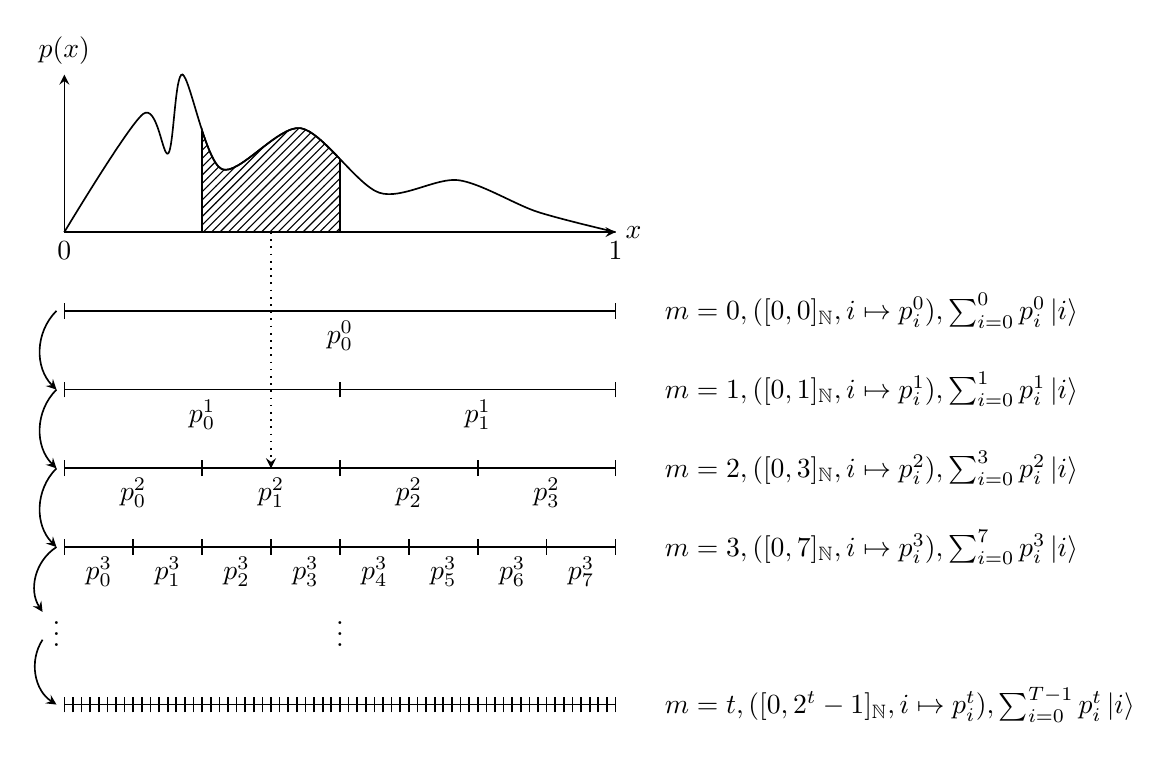
\begin{tikzpicture}[>=stealth, scale=2, semithick]
        \draw[pattern=north east lines] plot [smooth] coordinates { (0, 0) (0.5, 0.75) (0.66, 0.5) (0.75, 1) (1.0, 0.4) (1.5, 0.66) (2.0, 0.25) (2.5, 0.33) (3.0, 0.13) (3.5, 0) };
        \fill[white] (0, 0) -- (0.875, 0) -- (0.875, 1) -- (0, 1) -- cycle;
        \fill[white] (1.75, 0) -- (3.5, 0) -- (3.5, 1) -- (1.75, 1) -- cycle;
        \newcommand{\intervaldiv}[2]{
            \draw[-] (0, #1) -- (3.5, #1);
            \foreach \x in {0, 1, ..., #2} {
                \draw (3.5*\x/#2, #1-0.05) -- (3.5*\x/#2, #1+0.05);
            }
        };
        % NOTE: Rough definition due to time constraints.
        \newcommand{\intervaldivprobcap}[4]{
            \foreach \x in {0, ..., #4} {
                \node[below] at (3.5*\x/#3+3.5*1/2*1/#3, #1) {\(p^#2_\x\)};
            }
        };
        \draw[->] (0, 0) -- (0, 1) node[above, pos=1.0] {\(p(x)\)};
        \draw[->] (0, 0) -- (3.5, 0) node[below, pos=0.0] {\(0\)} node[below, pos=1.0] {\(1\)} node[right, pos=1.0] {\(x\)};
        \intervaldiv{-0.50}{1};
        \intervaldiv{-1.00}{2};
        \intervaldiv{-1.50}{4};
        \intervaldiv{-2.00}{8};
        \node at (1.75, -2.50) {\(\vdots\)};
        \intervaldiv{-3.00}{64};
        \intervaldivprobcap{-0.50}{0}{1}{0};
        \intervaldivprobcap{-1.00}{1}{2}{1};
        \intervaldivprobcap{-1.50}{2}{4}{3};
        \intervaldivprobcap{-2.00}{3}{8}{7};
        \node[right] at (3.75, -0.50) {\(m = 0, ([0, 0]_{\mathbb{N}}, i \mapsto p_i^0), \sum_{i=0}^0 p_i^0 \ket{i}\)};
        \node[right] at (3.75, -1.00) {\(m = 1, ([0, 1]_{\mathbb{N}}, i \mapsto p_i^1), \sum_{i=0}^1 p_i^1 \ket{i}\)};
        \node[right] at (3.75, -1.50) {\(m = 2, ([0, 3]_{\mathbb{N}}, i \mapsto p_i^2), \sum_{i=0}^3 p_i^2 \ket{i}\)};
        \node[right] at (3.75, -2.00) {\(m = 3, ([0, 7]_{\mathbb{N}}, i \mapsto p_i^3), \sum_{i=0}^7 p_i^3 \ket{i}\)};
        \node (1) at (-0.05, -2.50) {\(\vdots\)};
        \path[->] (-0.05, -0.50) edge[bend right=45] (-0.05, -1.00)
                  (-0.05, -1.00) edge[bend right=45] (-0.05, -1.50)
                  (-0.05, -1.50) edge[bend right=45] (-0.05, -2.00)
                  (-0.05, -2.00) edge[bend right=45] (1)
                  (1) edge[bend right=45] (-0.05, -3.00);
        \node[right] at (3.75, -3.00) {\(m = t, ([0, 2^t-1]_{\mathbb{N}}, i \mapsto p_i^t), \sum_{i=0}^{T-1} p_i^t \ket{i}\)};
        \draw plot [smooth] coordinates { (0, 0) (0.5, 0.75) (0.66, 0.5) (0.75, 1) (1.0, 0.4) (1.5, 0.66) (2.0, 0.25) (2.5, 0.33) (3.0, 0.13) (3.5, 0) };
        \draw[->, dotted] (1.3125, 0.00) -- (1.3125, -1.50);
        % Dirty approximation.
        \draw (0.875, 0) -- (0.875, 0.645);
        \draw (1.75, 0) -- (1.75, 0.46);
    \end{tikzpicture}
    \caption{Sketch for understanding the divisions. Here for \(t = 6\) and captions only in the first four divisions to avoid cluttering the sketch. The vertical axis has no markings as the image of the function \(p\) is drawn solely for illustration. On the right, the associated value of \(m\), the associated discrete probability space and the corresponding state are denoted. The arrows on the left illustrate the direction of the inductive algorithm by Grover and Harris. The part of the area under the curve of \(p\), which gives \(p_1^2\), has been highlighted.}
\end{figure}

\subsection{Quantum Mechanical Metrics \draftcommentgreen{DONE}}

\paragraph*{State Similarity} \phantom{}\\\phantom{}

Let \(\ket{\varphi}, \ket{\psi} \in \mathbb{C}^n\) be two quantum states for this part. To compare the similarity between them, one can use the introduced standard norm and define a metric by \(\norm{\ket{\varphi}-\ket{\psi}}\).

\begin{theorem}
    The tuple \((\{\ket{\psi} \in \mathbb{C}^n \mid \norm{\ket{\psi}} = 1\}, d_n)\) is a metric space, where \(d_n\) is the map
    \begin{align}
        d_n \colon \mathbb{C}^n \times \mathbb{C}^n \to \mathbb{R}_{\geq 0}, (\ket{\varphi}, \ket{\psi}) \mapsto \norm{\ket{\varphi}-\ket{\psi}}
    \end{align}
\end{theorem}

The proof can be found in \cite[p. 1-2]{Werner2018}, the definition of a metric can be found in \cite[p. 551]{Werner2018}. This theorem, to us, has semantical meaning. The complex vector norm induces a metric, meaning that we can measure the similarity between states by computing the above formula. A short rewrite yields the following theorem.

\begin{theorem} \label{state_similarity_theorem}
    It holds, that
    \begin{align}
        \norm{\ket{\varphi}-\ket{\psi}} = \sqrt{2(1-\Re(\braket{\varphi}{\psi}))}
    \end{align}
\end{theorem}

\begin{proof}
    We use the additivity of the complex standard product in both components and compute:
    \begin{align}
        \norm{\ket{\varphi}-\ket{\psi}}^2 &= \braket{\ket{\varphi}-\ket{\psi}}{\ket{\varphi}-\ket{\psi}}\\
        &= \braket{\varphi}{\varphi}-\braket{\psi}{\varphi}-\braket{\varphi}{\psi}+\braket{\psi}{\psi}\\
        &\overset{\ref{norm_rewrite_1}}{=} 2(1-\Re(\braket{\varphi}{\psi}))
    \end{align}
    \begin{enumerate}[label=(\arabic*)]
        \item \label{norm_rewrite_1} We use, that \(\norm{\ket{\varphi}}^2 = \norm{\ket{\psi}}^2 = 1\). Furthermore, we have
        \begin{align}
            \braket{\psi}{\varphi}+\braket{\varphi}{\psi} = \sum_{i=1}^n \varphi_i\psi_i^* + \sum_{i=1}^n \varphi_i^*\psi_i
        \end{align}
        However, \(\varphi_i\psi_i^* + \varphi_i^*\psi_i = 2\varphi_{i1}\psi_{i1} + 2\varphi_{i2}\psi_{i2}\). So \(\braket{\psi}{\varphi}+\braket{\varphi}{\psi} = 2\Re(\braket{\varphi}{\psi})\).
    \end{enumerate}
\end{proof}

\paragraph*{Operator Similarity} \phantom{}\\\phantom{}

Similarly to state similarity, there are norms for operators, which allow us to, for instance, analyze the error of a quantum algorithm. With \cite[p. 51]{Werner2018} in mind, we introduce the following theorem.

\begin{theorem} \label{operator_norm}
    The following map is a norm, the so-called \emph{operator norm}:
    \begin{align}
        \norm{\cdot}\colon \mathbb{C}^{n \times n} \to \mathbb{R}_{\geq 0}, A \mapsto \max_{\substack{\ket{\varphi} \in \mathbb{C}^n\\\norm{\ket{\varphi}} = 1}} \norm{A\ket{\varphi}}
    \end{align}
\end{theorem}

\begin{proof}
    Let \(S \coloneqq \{\ket{\varphi} \in \mathbb{C}^n \mid \norm{\ket{\varphi}} = 1\}\). The map is well-defined, since linear maps over \(\mathbb{C}^n\) are continuous and \(S\) is closed and bounded by definition wrt. the standard topology over \(\mathbb{C}^n\), thus by Heine-Borel \cite[p. 41]{Forster2017} compact. So the maximum always exists \cite[p. 43]{Forster2017}. To be precise, the closedness is due to one being able to span a line between a point outside of \(S\) and \(0\) and taking the distance to the point hit on \(S\) as the associated open set for the point, the boundedness, due to the fact, that \(\max\{\norm{\ket{v}}\} = 1 < 2\), so \(S \subset \{v \in \mathbb{C}^n \mid \norm{v} < 2\}\).
    
    The homogenity follows from \(\norm{(zA)\ket{\varphi}} = |z|\norm{A\ket{\varphi}}\), which carries over into the maximum. The triangle inequality also carries over from the norm of \(\mathbb{C}^n\). Lastly, the positive-definiteness is obtained by observing, that if the vectors of an arbitrary base are all mapped to zero, the linear map itself must be zero. This concludes the proof.
\end{proof}

\begin{example}
    Consider the operator given by
    \begin{align}
        A \coloneqq \begin{pmatrix}
            1 & 0\\
            i & 0
        \end{pmatrix}
    \end{align}
    Then for any \((b_1, b_2) \in \mathbb{C}^2\), \(\norm{A \begin{pmatrix}b_1 & b_2\end{pmatrix}^t}^2 = 2|b_1|^2\), so \(\norm{A} = \sqrt{2}\).
\end{example}

This norm also induces a metric, as the norm for states did.

\begin{remark}[Comparing Operators]
    To compare two operators \(U\) and \(U'\) and prove a bound for the operator distance \(\norm{U-U'}\), it suffices to bound the distance \(\norm{U\ket{\varphi}-U'\ket{\varphi}}\), with \(\ket{\varphi}\) being an arbitrary quantum state.
\end{remark}

\subsection{Qutrits \draftcommentgreen{DONE}} \label{subsection_qutrits}

Whilst qubits are the quantum equivalent of bits, \(\emph{qutrits}\) imitate the concept of a \(\emph{trit}\). Such electrical devices allow us to store three states, instead of two. In some systems, we denote them as \(0, 1, 2\) and in others in form of the \emph{balanced representation} \(-1, 0, 1\) for convenience \cite[p. 1]{Parhami_2013}. A qutrit is a member of \(\mathbb{C}^3\). We denote the canonical base as \(\{\ket{0}, \ket{1}, \ket{2}\}\) \cite[pp. 2-3]{Gokhale2019}.

We want to study three-dimensional rotations of qutrits. First, we give a lemma, which we derive from \cite[pp. 70-75]{Janich2010}.

\begin{definition}
    Let
    \begin{align}
        \times\colon \mathbb{R}^3 \times \mathbb{R}^3 \to \mathbb{R}^3, (u, v) \mapsto \begin{pmatrix}
            u_2v_3-u_3v_2\\
            u_3v_1-u_1v_3\\
            u_1v_2-u_2v_1
        \end{pmatrix}
    \end{align}
    be the so-called \emph{cross product}.
\end{definition}

\begin{lemma} \label{lemma_definition_cross_product}
    If \(\{u, v\} \subseteq \mathbb{R}^3\) is an orthonormal system, then \(\{u, v, u \times v\}\) is an orthonormal basis.
\end{lemma}

The proof can be found in the above-mentioned literature. When constructing three-dimensional unitaries, the cross product proves to be useful, as we will see in the proof of the following theorem.

\begin{theorem}[Three-Dimensional Qutrit Rotation] \label{qutrit_rotation}
    For a \(m \in \mathbb{N}_{\geq 1}\)-qubit-register with an appended qutrit and classically efficiently computable functions \(f\colon \mathbb{R} \to \mathbb{R}\), \(g\colon \mathbb{R} \to \mathbb{R}\), s.t. \(f^2+g^2 \leq 1\) and \(g^2(x) \neq 1\) for all \(x \in \mathbb{R}\), there is an efficient quantum algorithm, that achieves for any desirable precision
    \begin{align}
        \mathbb{C}^{2^m \cdot 3} \to \mathbb{C}^{2^m \cdot 3}, \ket{\lambda}\ket{0} \mapsto \ket{\lambda}(\sqrt{1-f^2(\lambda)-g^2(\lambda)}\ket{0}+f(\lambda)\ket{1}+g(\lambda)\ket{2})
    \end{align}
\end{theorem}

\begin{proof}
    We start off with a geometric argument on three-dimensional rotations. One notices, that the desired state of the qutrit is normalized, and that the amplitudes of the state vector are real. We can imagine the problem as moving the vector \(\ket{0}\) on the real unit sphere \(S^2\) into our target state, as depicted in \Cref{qutrit_rotation_figure}.
    
    We now directly explain, how to rotate the qutrit state \(\ket{0}\) into an arbitrary qutrit state of form \(\ket{\xi} \in \mathbb{R}^3\). Let \(P_{01} \coloneqq \ket{0}\bra{0} + \ket{1}\bra{1}\). \(\varphi \coloneqq \sphericalangle(\ket{0}, P_{01}\ket{\xi}), \psi \coloneqq \sphericalangle(P_{01}\ket{\xi}, \ket{\xi})\). Let \((\varphi, \psi) = (0, \pi/2)\), if \(\ket{\xi}_3 = 1\) and \((\varphi, \psi) = (0, 3\pi/2)\) for \(\ket{\xi}_3 = -1\). Note, that \(P_{01}\) performs the projection onto the plane spanned by \(\{\ket{0}, \ket{1}\}\). First, we rotate \(\ket{0}\) along the plane spanned by \(\{\ket{0}, \ket{1}\}\) by angle \(\varphi\). Then, we rotate the resulting vector \(P_{01}\ket{\xi}\) by the angle \(\psi\) along the plane spanned by \(\{P_{01}\ket{\xi}, \ket{2}\}\) into \(\ket{\xi}\).
    
    The two-dimensional standard rotation matrix, as seen in \Cref{controlled_rotation}, is for some \(\theta \in (-\pi, \pi]\)
    \begin{align}
        \begin{pmatrix}
            \cos(\theta) & -\sin(\theta)\\
            \sin(\theta) &  \cos(\theta)
        \end{pmatrix}
    \end{align}
    In three dimensions, we can always fix one coordinate and look at the cartesian coordinate system, that is spanned, when the canonical unit vector of the fixed coordinate points upwards and the others point downwards. Especially, \(\ket{2}\) is to the right of \(\ket{0}\). Otherwise, \(\ket{0}\) is right of \(\ket{1}\) and \(\ket{1}\) is right of \(\ket{2}\). To rotate in these induced planes, we look at the rotation matrices of form
    \begin{align}
        R_x(\theta) \coloneqq \begin{pmatrix}
                       1 &             0 &             0\\
                       0 &  \cos(\theta) & -\sin(\theta)\\
                       0 &  \sin(\theta) &  \cos(\theta)
        \end{pmatrix},
        R_y(\theta) \coloneqq \begin{pmatrix}
            -\sin(\theta) &             0 & \cos(\theta)\\
                        0 &             1 &            0\\
             \cos(\theta) &             0 & \sin(\theta)
        \end{pmatrix},
        R_z(\theta) \coloneqq \begin{pmatrix}
            \cos(\theta) & -\sin(\theta) & 0\\
            \sin(\theta) &  \cos(\theta) & 0\\
                       0 &             0 & 1
        \end{pmatrix}
    \end{align}
    Pay special note to \(R_y(\theta)\). We apply \(R_z(\varphi)\) to obtain
    \begin{align}
        \ket{0} = \begin{pmatrix}
            1\\
            0\\
            0
        \end{pmatrix} \mapsto \begin{pmatrix}
            \cos(\varphi)\\
            \sin(\varphi)\\
            0
        \end{pmatrix}
    \end{align}
    and then
    \begin{align}
        \begin{pmatrix}
            \cos(\varphi)\\
            \sin(\varphi)\\
            0
        \end{pmatrix} \mapsto \cos(\psi) \begin{pmatrix}
            \cos(\varphi)\\
            \sin(\varphi)\\
            0
        \end{pmatrix} + \sin(\psi) \ket{2} = \begin{pmatrix}
            \cos(\varphi)\cos(\psi)\\
            \sin(\varphi)\cos(\psi)\\
            \sin(\psi)
        \end{pmatrix}
    \end{align}
    To get geometrical intuition for this result, we can observe, that as we look at the latter described plane, the coefficients of this linear combination correspond to the lengths of the vectors for the final state. We want a unitary, which is able to rotate \(\ket{0}\) as described. In other words, we are searching for values \(\alpha, \beta, \gamma, \delta, \varepsilon, \zeta \in \mathbb{C}\), s.t. we have a unitary matrix of form
    \begin{align}
        \begin{pmatrix}
            \cos(\varphi)\cos(\psi) & \alpha      & \beta \\
            \sin(\varphi)\cos(\psi) & \gamma      & \delta \\
            \sin(\psi)              & \varepsilon & \zeta
        \end{pmatrix}
    \end{align}
    We can derive at least two such unitaries. First, observe, that the norm of the first column is \(1\), since \Cref{trigonometric_pythagoras} gives us:
    \begin{align}
        (\cos^2(\varphi)+\sin^2(\varphi))\cos^2(\psi)+\sin^2(\psi) = 1
    \end{align}
    By inspecting the coefficients closely, we suggest the vector:
    \begin{align}
        \begin{pmatrix}
            -\cos(\varphi)\sin(\psi)\\
            -\sin(\varphi)\sin(\psi)\\
            \cos(\psi)
        \end{pmatrix}
    \end{align}
    To form an orthonormal basis of a 2-dimensional subspace of \(\mathbb{C}^3\). And indeed, we have for the inner product
    \begin{align}
        \braket{\begin{array}{c}
            \cos(\varphi)\cos(\psi)\\
            \sin(\varphi)\cos(\psi)\\
            \sin(\psi)
        \end{array}}{\begin{array}{c}
            -\cos(\varphi)\sin(\psi)\\
            -\sin(\varphi)\sin(\psi)\\
            \cos(\psi)
        \end{array}} = -(\cos^2(\varphi)+\sin^2(\varphi))\cos(\psi)\sin(\psi)+\cos(\psi)\sin(\psi) = 0
    \end{align}
    The vector is also normalized, due to
    \begin{align}
        (\cos^2(\varphi)+\sin^2(\varphi))\sin^2(\psi)+\cos^2(\psi) = 1
    \end{align}
    In the above vector, we negated the first two components. One can also negate only the third one, but for \((\varphi, \psi) = (0, 0)\), that would give us \(-\ket{2}\). We choose the first version, due to preference. Furthermore, to construct the third vector, we can take cross product, see previously \Cref{lemma_definition_cross_product}, of both vectors to obtain a vector, that is orthogonal to both and even normalized. We have
    \begin{align}
        &\phantom{=} \begin{pmatrix}
            \cos(\varphi)\cos(\psi)\\
            \sin(\varphi)\cos(\psi)\\
            \sin(\psi)
        \end{pmatrix}
        \times
        \begin{pmatrix}
            -\cos(\varphi)\sin(\psi)\\
            -\sin(\varphi)\sin(\psi)\\
            \cos(\psi)
        \end{pmatrix}\\
        &= \begin{pmatrix}
            \sin(\varphi)\cos^2(\psi)+\sin^2(\psi)\sin(\varphi)\\
            -\sin^2(\psi)\cos(\varphi)-\cos(\varphi)\cos^2(\psi)\\
            -\cos(\varphi)\cos(\psi)\sin(\varphi)\sin(\psi)+\sin(\varphi)\cos(\psi)\cos(\varphi)\sin(\psi)
        \end{pmatrix} = \begin{pmatrix}
            \sin(\varphi)\\
            -\cos(\varphi)\\
            0
        \end{pmatrix}
    \end{align}
    The obtained vector is normalized and, with the other two vectors, forms an orthogonal base of \(\mathbb{C}^3\) with the other two vectors. We get the matrix
    \begin{align}
        R(\varphi, \psi) \coloneqq \begin{pmatrix}
            \cos(\varphi)\cos(\psi) & -\cos(\varphi)\sin(\psi) & \sin(\varphi)\\
            \sin(\varphi)\cos(\psi) & -\sin(\varphi)\sin(\psi) & -\cos(\varphi)\\
            \sin(\psi)              & \cos(\varphi)            & 0
        \end{pmatrix}
    \end{align}
    This matrix is unitary, according to our derivation and \Cref{theorem_unitary_matrices_characterization}. We turn to the original problem. Using the first column of the matrix, we get the desired condition:
    \begin{align}
        \ket{0} \mapsto \begin{pmatrix}
            \cos(\varphi)\cos(\psi)\\
            \sin(\varphi)\cos(\psi)\\
            \sin(\psi)
        \end{pmatrix} = \begin{pmatrix}
            \sqrt{1-f^2(\lambda)-g^2(\lambda)}\\
            f(\lambda)\\
            g(\lambda)
        \end{pmatrix}
    \end{align}
    From which we get \(\psi \coloneqq \arcsin(g(\lambda))\) and \(\varphi \coloneqq \arcsin\left(\frac{f(\lambda)}{\sqrt{1-g^2(\lambda)}}\right)\).

    Append \(n, o \in \mathbb{N}_{\geq 1}\) zeroed-out qubits to the first register and perform the map
    \begin{align}
        \ket{\lambda}\ket{0}\ket{0} \mapsto \ket{\lambda}\ket{\left(\arcsin\left(\frac{f(\lambda)}{\sqrt{1-g^2(\lambda)}}\right), \arcsin(g(\lambda))\right)}
    \end{align}
    Here, we have stored the approximations of \(\varphi\) and \(\psi\) in the two auxiliary registers. It is also clear, that we can denote such a tuple in binary via an arbitrary encoding format. We define a unitary of form
    \begin{align}
        \sum_{\theta = 0}^{2^o-1} \ket{\theta}\bra{\theta} \otimes R(0, \mathcal{F}(\theta)) + \sum_{\theta = 2^o}^{2^{n+o}-1} \ket{\theta}\bra{\theta} \otimes R(\mathcal{F}(\theta - 2^o), \mathcal{F}(\theta \bmod 2^o))
    \end{align}
    similar to the proof of \Cref{controlled_rotation}. This gives us the desired behavior of
    \begin{align}
        &\phantom{\mapsto} \ket{\lambda}\ket{\left(\arcsin\left(\frac{f(\lambda)}{\sqrt{1-g^2(\lambda)}}\right), \arcsin(g(\lambda))\right)} \ket{0}\\
        &\mapsto \ket{\lambda}\ket{0}\ket{0}(\sqrt{1-f^2(\lambda)-g^2(\lambda)}\ket{0}+f(\lambda)\ket{1}+g(\lambda)\ket{2})
    \end{align}
    by uncomputing the helper bits afterwards. It is clear, that the above instructions are all efficiently implementable. Thus, we are finished.
\end{proof}

\begin{remark}[On the Orientation of the Coordinate System]
    We have transformed cartesian system, spanned by \(\{\ket{0}, \ket{1}, \ket{2}\}\), into another one, spanned by \(\{\ket{0}, \ket{2}, -\ket{1}\}\), with the associated mappings of the canonical basis vectors in order of this enumeration. This may help visualize the transformation much better. Note that, furthermore, the vector product respects the \emph{right hand rule} \cite[pp. 70-75]{Janich2010}, related to Lenz's law from electrophysics \cite[pp. 314-315]{Griffiths}. By reversing the order in the vector product, we could obtain a map into the coordinate system, spanned by the vectors \(\{\ket{0}, \ket{2}, \ket{1}\}\), in this order, but we refrain from doing that.
\end{remark}

\tdplotsetmaincoords{90}{90}
\tdplotsetrotatedcoords{0}{22.5}{-22.5}
\begin{figure}[!hbtp]
    \centering
    \begin{tikzpicture}[>=stealth, scale=4, semithick, tdplot_rotated_coords]
        \draw[->] (0, 0, 0) -- (1, 0, 0) node[below left] {\(\ket{0}\)};
        \draw[->] (0, 0, 0) -- (0, 1, 0) node[right] {\(\ket{1}\)};
        \draw[->] (0, 0, 0) -- (0, 0, 1) node[above] {\(\ket{2}\)};
        \draw[->, dashed] (0, 0, 0) -- (0.7071, 0.7071, 0);
        \draw[->] (0, 0, 0) -- (0.3162, 0.3162, 0.8944) node[above right] {\(\ket{\xi}\)};
        \tdplotdrawarc[tdplot_rotated_coords, draw=none]{(0, 0, 0)}{0.25}{0}{45}{}{\(\varphi\)};
        \tdplotdrawarc[tdplot_rotated_coords, ->, dashed]{(0, 0, 0)}{0.5}{0}{45}{}{};

        \tdplotsetrotatedthetaplanecoords{45}
        \tdplotdrawarc[tdplot_rotated_coords, draw=none]{(0, 0, 0)}{0.25}{26.5651}{90}{}{\(\psi\)};
        \tdplotdrawarc[tdplot_rotated_coords, <-, dashed]{(0, 0, 0)}{0.5}{26.5651}{90}{}{};
    \end{tikzpicture}
    \caption{Rotating the qutrit state \(\ket{0}\) according to some angles \(\varphi, \psi \in (-\pi, \pi]\) into some state \(\ket{\xi} \in \mathbb{R}^3 \subset \mathbb{C}^3\). Here illustrated for \(\ket{\xi} \coloneqq \frac{1}{\sqrt{10}}(\ket{0}+\ket{1})+\frac{2}{\sqrt{5}}\ket{2}\), thus \(\varphi = \frac{\pi}{4}\) and \(\psi = \arcsin\left(\frac{2}{\sqrt{5}}\right)\).}
    \label{qutrit_rotation_figure}
\end{figure}

\subsection{Amplitude Amplification \draftcommentgreen{DONE}} \label{amplitude_amplification_section}

In 2000, Brassard et al. \cite[pp. 4-10]{Brassard2000} studied the problem of boosting the success probability of an arbitrary quantum algorithm, i.e., the probability of a measurement yielding a desired result. Inspired by the ideas from Grover et al., the researchers developed the so-called \emph{Amplitude Amplification} algorithm, to which this subsection is dedicated.

\paragraph*{Grovers Multi-Search Algorithm} \phantom{}\\\phantom{}

Grovers algorithm for a multi-search problem, as in \cite[pp. 140-155]{Homeister2018}, may be formulated the following way.

\begin{theorem}[Grovers Algorithm for a Multi-Search Problem] \label{grovers_algorithm_for_a_multi_search_problem}
    Given a function of form \(f\colon [0, N-1]_{\mathbb{N}} \to \{0, 1\}\), \(N \coloneqq 2^n\) with \(0 < |f^{-1}(1)| \eqqcolon M < N\), there exists a quantum algorithm, that can find an element from \(f^{-1}(1)\) in time \(\onot(\sqrt{N/M})\).
\end{theorem}

\begin{remark}[Form of \(f\)]
    If the cardinality of the domain of \(f\) is not a power of two, then \(f\) can be naturally extended to some function \(\hat{f}\) by extending the count to the next power of two and mapping all of the new domain values to zero.
\end{remark}

We want to now recall the idea of the multi-search version, as the version for single-search problems is naturally implied and works analogously. We shall further omit the analysis, as we will prove the more general case with AA. The structure of Grovers algorithm follows the following iteration: We first construct the uniform superposition state \(H^{\otimes n}\ket{0}\), initialize a helper qubit to \((H \circ \notgate)\ket{0}\) and then repeatedly apply the so-called \emph{Grover operator} \cite[p. 146]{Homeister2018}
\begin{align}
    G \coloneqq -H^{\otimes n}R_NH^{\otimes n}V_f \label{grover_operator}
\end{align}
exactly
\begin{align}
    G(N, M) \approx\frac{\pi}{4} / \arcsin\left(\sqrt{\frac{M}{N}}\right) - \frac{1}{2}
\end{align}
times \cite[p. 153-155]{Homeister2018}, where \(G(N, M) \in \mathbb{N}\) denotes the required number of iterations. As \(G(N, M) \in \onot(\sqrt{N/M})\) due to \Cref{sine_bound}, this gives the claimed runtime. In the analysis of Grovers algorithm, \(V_f\) is interpreted as the operator mirroring the amplitudes to be boosted wrt. \(0\), whilst \(-H^{\otimes n}R_NH^{\otimes n}\) mirrors all amplitudes wrt. the arithmetic mean of all amplitudes. This directly gives the geometric interpretation for the algorithm, that Grovers procedure successively rotates the uniform superposition state into the boosted state. The operators \(R_N, V_f \in \mathbb{C}^{N \times N}\) here are defined via the following actions on any canonical basis vector \(\ket{x}\) of \(\mathbb{C}^N\):
\begin{align}
    R_N\ket{x} \coloneqq \begin{cases}
        -\ket{x} & x = 0\\
        \phantom{-}\ket{x} & x \neq 0
    \end{cases} \qquad V_f\ket{x} \coloneqq \begin{cases}
        -\ket{x} & x \in f^{-1}(1)\\
        \phantom{-}\ket{x} & x \notin f^{-1}(0)
    \end{cases} \label{grover_mirroring_operations}
\end{align}
Let it be noted, that the required helper qubit is used by \(V_f\) and omitted here for simplicity. Denoting \(V_f\in \mathbb{C}^{N \times N}\) is thus technically wrong, but we do not loose any generality. Both gates can be efficiently implemented \cite[pp. 144-145]{Homeister2018}.

\paragraph*{The General Case} \phantom{}\\\phantom{}

Now to the more general case in AA. Consider a measurement-free (except for helper qubits) quantum algorithm acting on \(n\) qubits \(U \in \mathbb{C}^{N \times N}\) and a Boolean function \(\chi\colon \{0, 1\}^n \to \{0, 1\}\). Suppose we wish to measure the state \(\ket{\Psi} \coloneqq U\ket{0}\) wrt. the observable \(\{\Span(\{\ket{k} \mid k \in \chi^{-1}(0)\}), \Span(\{\ket{k} \mid k \in \chi^{-1}(1)\})\}\) to obtain the index of the subspace given by \(\chi^{-1}(1)\) with probability \(p \coloneqq \braket{P_1\ket{\Psi}}{P_1\ket{\Psi}} \in (0, 1)\) wlog., where \(P_i \coloneqq \sum_{x \in \chi^{-1}(i)}\ket{x}\bra{x}\) for \(i \in \mathbb{F}_2\). We especially want to boost that probability of success. The following formulation is directly based off the paper by Brassard et al..

\phantom{}

Denote \(\ket{\Psi_i} \coloneqq P_i\ket{\Psi}\) as well for \(i \in \mathbb{F}_2\). Initialize a \(n\)-qubit register to \(U\ket{0}\), and an ancilla qubit to \((H \circ \notgate)\ket{0}\), but we omit it as explained above. We now define an operator \(Q \in \mathbb{C}^{N \times N}\) via
\begin{align}
    Q \coloneqq -U R_N U^\dagger V_{\chi}
\end{align}
where \(V_{\chi}\) corresponds to \(V_f\) via \(f \coloneqq \chi\). This operator corresponds to a direct generalization of the Grover operator from \Cref{grover_operator}.

\begin{lemma} \label{aa_iteration_lemma}
    Let \(\theta_p \coloneqq \arcsin(\sqrt{p})\). After \(j \in \mathbb{N}\) iterations of \(Q\) on \(\ket{\Psi}\), we have
    \begin{align}
        Q^j\ket{\Psi} = \frac{1}{\sqrt{p}}\sin((2j+1)\theta_p)\ket{\Psi_1}+\frac{1}{\sqrt{1-p}}\cos((2j+1)\theta_p)\ket{\Psi_0}
    \end{align}
\end{lemma}

This result is presented in \cite[pp. 5-7]{Brassard2000}, we give the argument in more detail.

\begin{proof}
    The proof is divided into the following parts:
    \begin{enumerate}[label=(\roman*)]
        \item[\ref{aa_iteration_proof_1}] \label{aa_iteration_proof_summary_1} We first calculate the states \(Q\ket{\Psi_1}\) and \(Q\ket{\Psi_0}\), which will give us, that the operator only acts in the two-dimensional subspace \(\Span(\{\ket{\Psi_1}, \ket{\Psi_0}\})\).
        \item[\ref{aa_iteration_proof_2}] After rewriting \(Q\) wrt. the subspace spanned by the images from \Cref{aa_iteration_proof_summary_1}, we calculate its eigenvalues and thus span an eigenbasis for the mentioned subspace.
        \item[\ref{aa_iteration_proof_3}] The initial state \(\ket{\Psi}\) is rewritten in the subspace spanned by the eigenvectors, from which we can calculate \(Q^j\ket{\Psi}\).
    \end{enumerate}

    \begin{enumerate}[label=(\roman*)]
        \item \label{aa_iteration_proof_1} The behavior of \(Q\) on the states \(\ket{\Psi_0}\) and \(\ket{\Psi_1}\) is given by:
        \begin{align}
            Q\ket{\Psi_1} &\overset{\ref{aa_q_action_psi_1_1}}{=} U(E_N-2\ket{0}\bra{0})U^\dagger\ket{\Psi_1} \overset{\ref{aa_q_action_psi_1_2}}{=}\ket{\Psi_1} - 2\ket{\Psi}\bra{\Psi}\ket{\Psi_1} \overset{\ref{aa_q_action_psi_1_3}}{=} (1-2p)\ket{\Psi_1} - 2p \ket{\Psi_0}\\
            Q\ket{\Psi_0} &= -U(E_N-2\ket{0}\bra{0})U^\dagger\ket{\Psi_0} = -\ket{\Psi_0} + 2\ket{\Psi}\bra{\Psi}\ket{\Psi_0} \overset{\ref{aa_q_action_psi_1_4}}{=} 2(1-p)\ket{\Psi_1} + (1-2p)\ket{\Psi_0}
        \end{align}
        \begin{enumerate}[label=(\arabic*), wide]
            \item \label{aa_q_action_psi_1_1} Consider the definitions of \(V_\chi\) and \(R_N\) as in \Cref{grover_mirroring_operations}, from which we directly have \(R_N = E_N-2\ket{0}\bra{0}\).
            \item \label{aa_q_action_psi_1_2} Using \(UE_NU^\dagger=E_N\) and \(2U\ket{0}\bra{0}U^\dagger = 2U\ket{0}(U\ket{0})^\dagger = 2\ket{\Psi}\bra{\Psi}\).
            \item \label{aa_q_action_psi_1_3} By \(\ket{\Psi} = \ket{\Psi_1} + \ket{\Psi_0}\) and the orthogonality relations.
            \item \label{aa_q_action_psi_1_4} As \(\bra{\Psi}\ket{\Psi_0} = \bra{\Psi}(\ket{\Psi}-\ket{\Psi_1}) = 1-p\).
        \end{enumerate}
        We rewrite \(Q\) wrt. the space \(H_\Psi \coloneqq \Span(\{\ket{\Psi_1}, \ket{\Psi_0}\})\) as
        \begin{align}
            Q_\Psi \coloneqq \begin{pmatrix}
                1-2p & 2(1-p)\\
                 -2p & 1-2p
            \end{pmatrix}
        \end{align}
        Since \(\ket{\Psi} \in H_\Psi\), we may repeatedly apply \(Q\) and remain in \(H_\Psi\), as in Grovers algorithm.
        \item \label{aa_iteration_proof_2} We calculate the eigenvalues and eigenvectors of \(Q_\Psi\). The characteristic polynomial gives via Sarrus' rule
        \newcommand{\lpm}{\lambda_\pm}
        \begin{align}
            \det(Q_\Psi - \lpm E_2) = (1-2p-\lpm)^2+4p(1-p) = \lpm^2-2(1-2p)\lpm+1
        \end{align}
        and by that
        \begin{align}
            \lpm &= (1-2p) \pm \sqrt{(1-2p)^2-1} = 1 \pm i 2 \sqrt{p}\sqrt{1-p}-2p\\
            &\overset{\ref{aa_q_eigenvalues_1}}{=} \cos^2(\theta_p)+\sin^2(\theta_p) \pm i 2 \sin(\theta_p)\cos(\theta_p) - 2 \sin^2(\theta_p)\\
            &= (\cos(\theta_p) \pm i\sin(\theta_p))^2 = e^{\pm i 2 \theta_p}
        \end{align}
        
        \begin{enumerate}[label=(\arabic*), wide]
            \item \label{aa_q_eigenvalues_1} Define \(\theta_p \coloneqq \arcsin(\sqrt{p}) \in [0, \pi/2]\) and use \Cref{trigonometric_pythagoras}.
        \end{enumerate}
        
        To obtain an eigenvector base for \(H_\Psi\), consider the SLE \((Q_\Psi - \lpm E_2)\ket{\Psi_\pm} = 0\) for some \(\ket{\Psi_\pm} \coloneqq \alpha_\pm \ket{\Psi_1} + \beta_\pm \ket{\Psi_0}\) with \(\alpha_\pm, \beta_\pm \in \mathbb{C}\). We handle both \(\lambda_+\) and \(\lambda_-\) in one calculation. Considering, that
        \begin{align}
            1-2p-\lpm = 1-2p-(\sqrt{1-p} \pm i\sqrt{p})^2 = \mp i 2 \sqrt{p}\sqrt{1-p} \label{expanded_lpm_appearing}
        \end{align}
        and dividing the SLEs first two rows by \(2\sqrt{1-p}\) and \(2\sqrt{p}\) respectively, we rewrite the SLE as
        \begin{align}
            \begin{pmatrix}
                \mp i\sqrt{p} & \sqrt{1-p}\\
                -\sqrt{p} & \mp i \sqrt{1-p}
            \end{pmatrix} \begin{pmatrix}
                \alpha_\pm\\
                \beta_\pm\\
            \end{pmatrix} = \begin{pmatrix}
                0\\
                0
            \end{pmatrix}
        \end{align}
        Wlog. setting \(\alpha_\pm \coloneqq 1/\sqrt{2p}\), we obtain
        \begin{align}
            \begin{pmatrix}
                \mp \frac{i}{\sqrt{2}}+\sqrt{1-p}\beta_\pm\\
                -\frac{1}{\sqrt{2}} \mp i\sqrt{1-p}\beta_\pm
            \end{pmatrix} = \begin{pmatrix}
                0\\
                0
            \end{pmatrix}
        \end{align}
        and thus \(\beta_\pm = \pm \frac{i}{\sqrt{2}}\frac{1}{\sqrt{1-p}}\). An eigenbasis of \(H_\Psi\) is thus composed of the eigenvectors
        \begin{align}
            \ket{\Psi_\pm} \coloneqq \alpha_\pm\ket{\Psi_1} + \beta_\pm\ket{\Psi_0} = \frac{1}{\sqrt{2}} \left(\frac{1}{\sqrt{p}}\ket{\Psi_1} \pm \frac{i}{\sqrt{1-p}}\ket{\Psi_0} \right)
        \end{align}
        \item \label{aa_iteration_proof_3} Rewriting \(\ket{\Psi}\) in these eigenbasis vectors gives using the square root of the full form of \(\lpm\) as in \Cref{expanded_lpm_appearing}, i.e. \(\sqrt{\lpm} = \sqrt{1-p} \pm i\sqrt{p} = e^{i\theta_p}\), gives
        \begin{align}
            \ket{\Psi} = \ket{\Psi_1} + \ket{\Psi_0} = \sqrt{\frac{p}{2}} (\ket{\Psi_+} + \ket{\Psi_-}) + \frac{1}{i} \sqrt{\frac{1-p}{2}} (\ket{\Psi_+} - \ket{\Psi_-}) = \frac{-i}{\sqrt{2}}(e^{i\theta_p}\ket{\Psi_+}-e^{-i\theta_p}\ket{\Psi_-})
        \end{align}
        As \(\ket{\Psi_+}\) and \(\ket{\Psi_-}\) are eigenvectors of \(Q_\Psi\), we thus have
        \begin{align}
            Q_\Psi^j\ket{\Psi} &= \frac{-i}{\sqrt{2}}\left(\frac{1}{\sqrt{2p}}(e^{i(2j+1)\theta_p}-e^{-i(2j+1)\theta_p})\ket{\Psi_1}+\frac{i}{\sqrt{2(1-p)}}(e^{i(2j+1)\theta_p}+e^{-i(2j+1)\theta_p})\ket{\Psi_0}\right)\\
            &= \frac{-i}{2\sqrt{p}}(2i)\sin((2j+1)\theta_p)\ket{\Psi_1} + \frac{1}{2\sqrt{1-p}}(2)\cos((2j+1)\theta_p)\ket{\Psi_0}\\
            &= \frac{1}{\sqrt{p}}\sin((2j+1)\theta_p)\ket{\Psi_1}+\frac{1}{\sqrt{1-p}}\cos((2j+1)\theta_p)\ket{\Psi_0}
        \end{align}
    \end{enumerate}
    This concludes the proof.
\end{proof}

Assuming, that we know the success probability \(p\), we can directly use \Cref{aa_iteration_lemma} to determine the number of iterations needed for producing a state close to \(\ket{\Psi_1}\). The condition
\begin{align}
    \sin^2((2j+1)\theta_p) \approx 1
\end{align}
for the success probablity of the state \(Q^j\ket{\Psi}\) can be optimized by letting approximately \(j \coloneqq \lfloor \pi / (4 \theta_p) \rfloor\). As \(\theta_p = \arcsin(\sqrt{p}) > \sqrt{p}\) following \Cref{sine_bound}, we thus have a runtime of \(\onot(1/\sqrt{p})\).\footnote{Even \(\Theta(1/\sqrt{p})\) for this general case due to lower-bound results for Grovers Algorithm, in which we will not dive into in this thesis.}

\phantom{}

We now want to consider the case in which \(p\) is unknown \cite[pp. 8-10]{Brassard2000}. The idea by Brassard et al. is to uniformly choose a number of applications of \(Q\), which is exponentially bounded. To be precise, consider the following algorithm.

{\centering\begin{minipage}{\linewidth}
    \begin{algorithm}[H]
        \caption{\textsc{Amplitude Amplification}}
        \label{amplitude_amplification}
        \begin{algorithmic}[1]
            \Require A unitary \(U \in \mathbb{C}^{N \times N}\), with \(N \coloneqq 2^n\), \(n \in \mathbb{N}_{\geq 1}\), as well as a function \(\chi\colon [0, N-1]_{\mathbb{N}} \to \{0, 1\}\) with \(\chi^{-1}(1) \notin \{\emptyset, [0, N-1]_{\mathbb{N}}\}\).
            \Ensure A quantum state \(\ket{\Psi} \in \mathbb{C}^N\), where the measurement of \(U\ket{0}\) wrt. the observable \(\{\Span(\mathcal{B}_0), \Span(\mathcal{B}_1)\}\) with \(\mathcal{B}_i \coloneqq \{\ket{x} \mid x \in \chi^{-1}(i)\}\) for \(i \in \mathbb{F}_2\) yielded a \(1\).
            \State Let \(l \coloneqq 0\), \(M \coloneqq 0\) and let \(c \in (1, 2)\) be arbitrary, but fixed.
            \While{true}
                \State \(l \gets l+1\), \(M \gets \lceil c^l \rceil\)
                \State Initialize \(\ket{\Psi} \coloneqq U\ket{0} \in \mathbb{C}^N\), while considering the necessary ancilla qubit.
                \State Measure \(\ket{\Psi}\) wrt. \(\{\Span(\mathcal{B}_0), \Span(\mathcal{B}_1)\}\), obtaining an index \(z \in \mathbb{F}_2\). \label{aa_first_measurement}
                \If{\(z = 1\)}
                    \State \Return{\(\ket{\Psi}\)}
                \Else
                    \State Initialize \(\ket{\Psi'} \coloneqq U\ket{0} \in \mathbb{C}^N\), while considering the necessary ancilla qubit.
                    \State Pick some \(j \in [1, M]_{\mathbb{N}}\) uniformly at random. \label{aa_laplacian_step}
                    \State \(\ket{\Psi'} \gets Q^j\ket{\Psi'}\)
                    \State Measure \(\ket{\Psi'}\) wrt. \(\{\Span(\mathcal{B}_0), \Span(\mathcal{B}_1)\}\), obtaining an index \(z' \in \mathbb{F}_2\). \label{aa_second_measurement}
                    \If{\(z' = 1\)}
                        \State{\Return \(\ket{\Psi'}\)}
                    \Else
                        \State Go to step 3.
                    \EndIf
                \EndIf
            \EndWhile
        \end{algorithmic}
    \end{algorithm}
\end{minipage}\par} \phantom{}

For the analysis, we need the following lemma.

\begin{restatable}{lemma}{aacosinehelpersumlemma} \label{aa_cosine_helper_sum_lemma}
    For any \(\alpha \in \mathbb{C}\) and \(m \in \mathbb{N}_{\geq 1}\), we have
    \begin{align}
        \sum_{j=0}^{m-1} \cos((2j+1)\alpha) = \frac{\sin(2m\alpha)}{2\sin(\alpha)}
    \end{align}
\end{restatable}

This lemma is taken from lemma 1 of a previous work on tight bounds for Grovers algorithm by Brassard and Boyer et al. \cite[p. 3]{Boyer_1998}. A similar analysis to the one presented in \cite[pp. 9-10]{Brassard2000} is given there. We prove the lemma in the appendix, see \Cref{aa_cosine_helper_sum_lemma_proof}.

\begin{lemma}
    \Cref{amplitude_amplification} runs in time \(\onot\left(\frac{1}{\sqrt{p}}\right)\).
\end{lemma}

\begin{proof}
    We use the notation as in \Cref{aa_iteration_lemma} and \Cref{amplitude_amplification}. Analyzing the number of calls directly turns out to be quite difficult due to the Laplacian experiment in step \Cref{aa_laplacian_step}. Brassard et al. thus suggest the following proof strategy: The expected probability of success in \Cref{aa_second_measurement} is first lower-bounded and then the variable \(l\) is split at a point \(M_0 \in \mathbb{N}\), chosen in dependence of \(\theta_p\) and \(c\). We then argue that both until \(M_0\) is reached and afterwards, we require \(\onot\left(\frac{1}{\sqrt{p}}\right)\) applications of \(Q\).

    First, consider the case, where \(p \geq 1/4\). Then the expected number of calls to \Cref{aa_first_measurement} is
    \begin{align}
        \sum_{n=0}^\infty (1-p)^n \geq \sum_{n=0}^\infty \frac{3}{4^n} = 4
    \end{align}
    due to \Cref{geometric_sum}.

    Assume \(p < 1/4\). Let \(l \in \mathbb{N}_{\geq 1}\) be fixed and \(M \coloneqq \left\lceil c^l \right\rceil\). Let \(X\colon [1, M]_{\mathbb{N}} \to [0, 1], j \mapsto \frac{1}{p}\sin^2((2j+1)\theta_p)\) denote the Laplacian random variable assigning each \(j\) the success probability of \Cref{aa_second_measurement} as in \Cref{aa_iteration_lemma}. Then
    \begin{align}
        \expectation[X] &= \sum_{j=1}^M \frac{1}{M} \frac{1}{p} \sin^2((2j+1)\theta_p) \overset{\ref{aa_analysis_helper_calc_1}}{=} \frac{1}{2p} \left(1-\frac{1}{M}\sum_{j=1}^M \cos((2j+1)(2\theta_p))\right)\\
        &\overset{\ref{aa_analysis_helper_calc_2}}{=} \frac{1}{2p}\left(1 - \frac{1}{2M}\frac{\sin(4(M+1)\theta_p)}{\sin(2\theta_p)} + \frac{1}{M} \cos(2\theta_p)\right)\\
        &\overset{\ref{aa_analysis_helper_calc_3}}{>} \frac{1}{2}\left(1-\frac{1}{2M}\frac{\sin(4(M+1)\theta_p)}{\sin(\theta_p)}\right) \overset{\ref{aa_analysis_helper_calc_4}}{=} \frac{1}{2}\left(1-\frac{1}{2M\sqrt{p}}\right)
    \end{align}
    \begin{enumerate}[label=(\arabic*)]
        \item Using \Cref{some_trigonometry_lemma}. \label{aa_analysis_helper_calc_1}
        \item Using \Cref{aa_cosine_helper_sum_lemma}. \label{aa_analysis_helper_calc_2}
        \item Consider the strict monotonicity of \(\sqrt{\cdot}\) and \(\arcsin\) in \((0, 1]\). So \(\theta_p \in (0, \arcsin(1/2))\). Use \(\sin(2x) > \sin(x)\) for \(x \in (0, \pi / 4] \supset (0, \arcsin(1/2))\), as the sine is strictly monotonous in \([0, \pi/2]\). Use \(p \in (0, 1)\) as well. Also use \(\evalat{\cos}{[0, \pi/2]} > 0\). \label{aa_analysis_helper_calc_3}
        \item By the definition of \(\theta_p\), see \Cref{aa_iteration_lemma}, we have \(\sin(\theta_p) = \sqrt{p}\). \label{aa_analysis_helper_calc_4}
    \end{enumerate}
    We shall from now on continue with the expected probability for success in \Cref{aa_second_measurement}. Whether the resulting lower bound is an actual probability solely depends on the value of \(l\), so we may derive the condition
    \begin{align}
        \frac{1}{2}\left(1-\frac{1}{2M\sqrt{p}}\right) \in [0, 1] \leadsto \frac{1}{2\sqrt{p}} \leq c^l \leq M^l \leadsto l \geq \log_c\left(\frac{1}{2\sqrt{p}}\right) \label{aa_lower_bound_becomes_probability}
    \end{align}
    This observation leads to the following approach for the analysis: Until the condition in \Cref{aa_lower_bound_becomes_probability} holds, we may iterate \(\lceil\log_c(1/(2\sqrt{p}))\rceil\) times, requiring at most
    \begin{align}
        \sum_{l=1}^{\left\lceil \log_c\left(\frac{1}{2\sqrt{p}}\right) \right\rceil} \left\lceil c^l \right\rceil &\leq \sum_{l=0}^{\left\lceil \log_c\left(\frac{1}{2\sqrt{p}}\right) \right\rceil} (c^l + 1) = \frac{1-c^{\left\lceil \log_c\left(\frac{1}{2\sqrt{p}}\right) \right\rceil+1}}{1-c}+\left\lceil \log_c\left(\frac{1}{2\sqrt{p}}\right) \right\rceil\\
        &\leq \frac{1-\frac{c^2}{2\sqrt{p}}}{1-c}+\left\lceil \log_c\left(\frac{1}{2\sqrt{p}}\right) \right\rceil \in \onot\left(\frac{1}{\sqrt{p}}\right)
    \end{align}
    calls to \(Q\) using \Cref{geometric_sum}. Let \(M_0 \coloneqq c^{\left\lceil \log_c\left(\frac{1}{2\sqrt{p}}\right) \right\rceil}\). We have analyzed the asymptotic number of calls to \(Q\) until \(M\) has reached or surpassed \(M_0\). After that, \(c^l = M_0c^i\) with \(i \coloneqq l - \left\lceil \log_c\left(\frac{1}{2\sqrt{p}}\right) \right\rceil \geq 1\). By bounding \(M_0 > \frac{1}{2\sqrt{p}}\) and \(M > M_0c^i\), we have a lower bound for the success probability of \Cref{aa_second_measurement} by
    \begin{align}
        \expectation[X] > \frac{1}{2}\left(1-\frac{1}{2M_0c^{i}\sqrt{p}}\right) > \frac{1}{2}\left(1-\frac{1}{c^i}\right)
    \end{align}
    The complementary event, by the previous argument, is bounded from above by \(1-\expectation[X] \leq \frac{1}{2}\left(1+\frac{1}{c^i}\right)\). Consider the condition \(\frac{c}{2}\left(1+\frac{1}{c^i}\right) < 1\), which gives \(i > \log_c\left(\frac{c}{2-c}\right)\). Now looking at the expectation value of the geometric random variable counting the calls of \(Q\) after \(M > M_0\), which is roughly \(\sum_{i=1}^\infty M_0c^i \left(\frac{1}{2}\left(1+\frac{1}{c^i}\right)\right)^i\), we may conclude the statement, as after \(\onot(1)\) many steps involving \(\onot(M_0)\) applications of \(Q\) each, \(\frac{c}{2}\left(1+\frac{1}{c^i}\right) < 1\), where we can bound the limit of the associated geometric series by \(\onot(M_0)\). So we require a total of \(\onot(M_0) = \onot(1/\sqrt{p})\) calls to \(Q\), concluding the argument.
\end{proof}

\begin{theorem}[Amplitude Amplification] \label{amplitude_amplification_theorem_unknown_probability}
    Given a measurement-free quantum algorithm \(U \in \mathbb{C}^{N \times N}\), \(N \coloneqq 2^n\), \(n \in \mathbb{N}\), which succeeds, i.e., gives a normalized projection into a subspace spanned by desirable basis vectors, with a possibly a priori unknown probability \(p \in (0, 1)\), we can perform a successful measurement using a quantum algorithm, that requires a runtime of \(\onot(1/\sqrt{p})\).
\end{theorem}

\begin{corollary}
    \Cref{grovers_algorithm_for_a_multi_search_problem} follows, especially for the case, when \(M\) is unknown. Consider \(\chi \coloneqq f\) and the unitary \(U \coloneqq H^{\otimes n}\) and the quantum algorithm, that initializes \(U\ket{0} = \frac{1}{\sqrt{N}}\sum_{i=0}^{N-1}\ket{i}\). Then measuring wrt. the observable \(\{\Span(\mathcal{B}_0), \Span(\mathcal{B}_1)\}\) with the notation as in \Cref{amplitude_amplification} succeeds with probability \(M/N\). Finding an element from \(f^{-1}(1)\) thus requires \(\onot(\sqrt{N/M})\) applications of \(Q\) using AA. Note, that after the measurement, we need to measure again wrt. the observable \(\{\Span(\ket{x}) \mid x \in \{0, 1\}^n\}\), as the state is then in \(\Span(\mathcal{B}_1)\).
\end{corollary}

\begin{corollary}
    AA is analogously applicable in the case, where qutrits are used inside of the algorithm of concern, as we only have to adjust the operator \(Q\) and consider in the analysis, that the Boolean function maps from the qubit-qutrit canonical basis vector indices into \(\{0, 1\}\).
\end{corollary}

\subsection{Quantum Phase Estimation  \draftcommentgreen{DONE}}

\begin{problem}
    Let \(U \in \mathbb{C}^{N \times N}\), \(N \coloneqq 2^n\), \(n \in \mathbb{N}_{\geq 1}\), be a unitary matrix with an eigenstate \(\ket{b} \in \mathbb{C}^N\) of phase \(\theta \in [0, 1)\). The problem of calculating or approximating \(\theta\) is called \emph{quantum phase estimation} (QPE).
\end{problem}

There is a general algorithm to this problem. The following theorem summarizes this classical result, which can be found in \cite[pp. 221-226]{Nielsen2010}. \Cref{qpe} shows the circuit diagram of the general QPE algorithm.

\begin{theorem}[General Quantum Phase Estimation]
    Let \(\varepsilon \in (0, 1)\), \(n \in \mathbb{N}_{\geq 1}\), \(N \coloneqq 2^n\) and
    \begin{align}
        t \geq n + \left\lceil \log\left(2+\frac{1}{2\varepsilon}\right) \right\rceil
    \end{align}
    Given a unitary \(U \in \mathbb{C}^{N \times N}\), an eigenstate \(\ket{b} \in \mathbb{C}^N\) of \(U\), an oracle for calculating the controlled unitaries \(\hat{U}^{\left(2^k\right)}\colon \mathbb{C}^{2 \cdot N} \to \mathbb{C}^{2 \cdot N}\) achieving \(\ket{0}\ket{b} \mapsto (\ket{0}+e^{2 \pi i (2^k \theta)}\ket{1})\ket{b}\) for arbitrary \(k \in [0, 2^{t-1}]_{\mathbb{N}}\) and a unitary gate \(\mathcal{B} \in \mathbb{C}^{N \times N}\) with \(\mathcal{B}\ket{0} = \ket{b}\) and potentially asymptotic time complexity \(T_{\mathcal{B}}\), we can approximate the phase of the associated eigenvalue of \(\ket{b}\) using \(t\) bits with \(\Theta(T_{\mathcal{B}} + t^2)\) operations and a success probability of at least \(1 - \varepsilon\).
\end{theorem}

\begin{figure}[!hbtp]
    \centering
    \begin{quantikz}
        \lstick{\(\ket{0}\)} \qw & \gate{H} \qw & \ctrl{4} & \qw & \qw \; ... \; & \qw & \qw \rstick{\(\frac{1}{\sqrt{2}}\left(\ket{0}+e^{2 \pi i (2^0) \theta}\ket{1}\right)\)}\\
        \lstick{\(\ket{0}\)} \qw & \gate{H} \qw & \qw & \ctrl{3} & \qw \; ... \; & \qw & \qw \rstick{\(\frac{1}{\sqrt{2}}\left(\ket{0}+e^{2 \pi i (2^1) \theta}\ket{1}\right)\)}\\
        & & & & ...\\
        \lstick{\(\ket{0}\)} \qw & \gate{H} \qw & \qw & \qw & \qw \; ... \; & \ctrl{1} & \qw \rstick{\(\frac{1}{\sqrt{2}}\left(\ket{0}+e^{2 \pi i (2^{t-1}) \theta}\ket{1}\right)\)}\\
        \lstick{\(\ket{0}\)} \qw & \gate{\mathcal{B}}\qw & \gate{\hat{U}^{\left(2^0\right)}} & \gate{\hat{U}^{\left(2^1\right)}} & \qw \; ... \; & \gate{\hat{U}^{\left(2^{t-1}\right)}} & \qw \rstick{\(\ket{b}\)}
    \end{quantikz}
    \caption{Circuit diagram for the first part of the general QPE algorithm. The \(t \in \mathbb{N}_{\geq 1}\) qubits are used to approximate a binary representation of the eigenvalue phase, as we can see on the right. The essential point of the first part is to store the vector \(\bigotimes_{k = 0}^{2^t-1} \left(\ket{0}+e^{2 \pi i (2^k) \theta}\ket{1}\right) \ket{b} = \frac{1}{\sqrt{2^t}} \sum_{j=0}^{2^t-1}\ket{j}U^j\ket{b}\), as one can recognize by aligning the binary representation of the summed up factor in the amplitude exponent with the canonical state for each possible product taken. Replication of \cite[pp. 221-226]{Nielsen2010}.}
    \label{qpe_first_part}
\end{figure}

\begin{figure}[!hbtp]
    \centering
    \begin{quantikz}
        \lstick{\(\ket{0}\)} \qw & \gate{H^{\otimes n}} \qw & \gate[wires=2]{\frac{1}{\sqrt{2^t}} \sum_{j=0}^{2^t-1}\ket{j}\ket{b} \mapsto \frac{1}{\sqrt{2^t}} \sum_{j=0}^{2^t-1}\ket{j}U^j\ket{b}} & \gate{\qft^\dagger} & \meter{\(\approx \theta\)}\\
        \lstick{\(\ket{0}\)} \qw & \gate{\mathcal{B}}   \qw & \qw & \qw & \rstick{\(\ket{b}\)} \qw
    \end{quantikz}
    \caption{Circuit diagram for the general QPE algorithm.}
    \label{qpe}
\end{figure}

\begin{remark} Consider, that
    \begin{itemize}
        \item this subsection was designated to showcase the most commonly seen QPE algorithm, but it will be of no further interest for the remaining thesis, as we will use different custom routines for phase estimation later on.
        \item the algorithm stores the approximation in a register to be measured, which may make it unsuitable for a subroutine in a larger algorithm. Furthermore, the requirement for the existence of the controlled exponential unitaries of \(U\) may be very restrictive.
    \end{itemize}
\end{remark}

\subsection{Hamiltonian Simulation  \draftcommentgreen{DONE}} \label{hamiltonian_simulation}

Consider our initial discussion on QM in \Cref{intro_to_quant_comp}. The time postulate in our form of interest was given in \Cref{time_postulate}. Since for a unitary \(H \in \mathbb{C}^{n \times n}\) and a time \(t \in \mathbb{R}_{\geq 0}\), we have, that \(e^{iHt}\) is unitary via \Cref{exponential_of_hermitian_is_unitary}, we can speak of particles, which evolve according to such a matrix exponential of a Hamiltonian, so for a quantum particle with state \(\ket{\psi(\cdot)}\), we could have
\begin{align}
    \ket{\psi(t)} = e^{iHt} \ket{\psi(0)}
\end{align}
for one such time \(t\). In the context of qubits, we may reformulate this fact as the following problem.

\begin{problem} \label{problem_hamiltonian_evolution}
    Let \(H \in \mathbb{C}^{N \times N}\), \(N \coloneqq 2^n\), be Hermitian and \(t \in \mathbb{R}_{\geq 0}\). The problem of applying the unitary operator \(e^{iHt}\) to a state \(\ket{\psi} \in \mathbb{C}^N\) is called \emph{Hamiltonian simulation}.
\end{problem}

This problem is in a very active state of research and has yielded a lot of results over the years, some notable mentions are \cite{Berry2015,Zhao2021}. Especially the Hamiltonian simulation with Hermitian operators in infinite-dimensional Hilbert spaces is of interest for general particle physics, QM and also for Quantum Chemistry, as it allows the simulation of the development of molecules, which in turn has multiple applications like the development of pharmaceuticals \cite[pp. 14-18]{Cao_2019}\footnote{Note, that the Hamiltonians are approximated in a real setting.}. We are especially interested in a comparatively old result by Berry et al. \cite{Berry2005}, which draws results from the same paper we referenced for the problem of quantum state generation by Aharonov et al. \cite{Aharonov2003}.

\phantom{}

One approach to \Cref{problem_hamiltonian_evolution} may be to approximate \(e^{iHt}\) directly by the associated Taylor series as in \Cref{definition_matrix_exponential_function}, but such an approach has been proven to not be satisfactory in practice \cite[p. 206]{Nielsen2010}, although some voices \cite[p. 1]{Zhao2021} argue, that this commonly presented perspective is too pessimistic. Here, we consider techniques based on decomposing the Hamiltonian into a sum of Hamiltonians \(H = \sum_{j=1}^m H_j\) and then individually simulating \(H_1, ..., H_m\) for \(m \in \mathbb{N}_{\geq 1}\). The main problem of using this idea directly is that the Hamiltonians may not commute, which violates \Cref{matrix_exponential_properties}. Instead, we compute an approximation of the so-called \emph{Trotter formula}.

\begin{theorem}[Trotter Formula] \label{trotter_formula}
    For Hamiltonians \(A, B \in \mathbb{C}^{n \times n}\) and \(t \in \mathbb{R}_{\geq 0}\), we have
    \begin{align}
        e^{i(A+B)t} = \lim_{m \to \infty} (e^{iAt/m}e^{iBt/m})^m
    \end{align}
\end{theorem}

Note that we explicitely do not require commuting operators here. We can also omit \(i\) and \(t\), but it suits our context. The proof is can be found in \cite[p. 207]{Nielsen2010}. Writing a sum of Hamiltonians in such a form is also the basic idea of the constructions used by Berry et al..

\phantom{}

We now consider sparse Hamiltonians, according to \Cref{sparse_and_efficiently_row_computable_matrices}. Let \(H \in \mathbb{C}^n\) be an \(s\)-sparse, efficiently row computable Hamiltonian, where \(s \in \mathbb{N}\). We first decompose the Hamiltonian into easily simulatable Hamiltonians, and then apply a recursion formula found by the researcher Suzuki, which is in turn based on the Trotter formula. As each Hamiltonian is easily simulatable, and we have approximately equality, we obtain the required simulation. The idea can be illustrated via the following sketch, which resembles a commutative diagram.

\begin{minipage}{\linewidth}
    \centering
    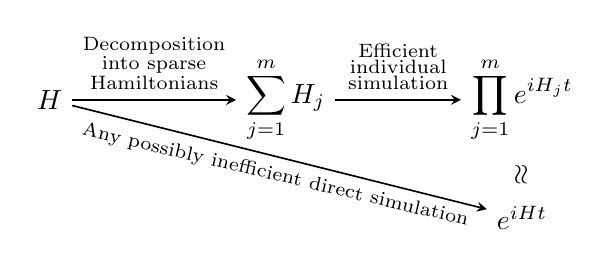
\begin{tikzpicture}[>=stealth, semithick]
        \node (0) at (0, 0) {\(H\)};
        \node (1) at (3, 0) {\(\displaystyle\sum_{j=1}^m H_j\)};
        \node (2) at (6, 0) {\(\displaystyle\prod_{j=1}^m e^{iH_jt}\)};
        \node (3) at (6, -1.5) {\(e^{iHt}\)};
        \draw[->] (0) -- (1) node[above, pos=0.5] {\(\substack{\text{Decomposition}\\\text{into sparse}\\\text{Hamiltonians}}\)};
        \draw[->] (1) -- (2) node[above, pos=0.5] {\(\substack{\text{Efficient}\\\text{individual}\\\text{simulation}}\)};
        \path[white!100] (2) edge node[black!100, rotate=90] {\(\approx\)} (3);
        \draw[->] (0) -- (3) node[below, pos=0.5, rotate=-13.2826] {\(\substack{\text{Any possibly inefficient direct simulation}}\)};
    \end{tikzpicture}
\end{minipage}

\begin{definition}
    The \emph{iterated logarithm} is defined as
    \begin{align}
        \log_2^*\colon \mathbb{R}_{> 0} \to \mathbb{N}, x \mapsto \begin{cases}
            0 & x \leq 1\\
            \min\left\{ i \in \mathbb{N}_{\geq 1} \; \middle| \; (\underbrace{\log_2 \circ ... \circ \log_2}_{i \text{ times}})(x) \leq 1 \right\} & x > 1
        \end{cases}
    \end{align}
\end{definition}

\begin{example} \label{iterated_logarithm_example}
    Whilst the iterated logarithm is a monotonically increasing function with discrete values, it grows incredibly slow. A textbook example is \(\log_2^*(2^{65536}) = 5\), which is a problem size, that is much greater than \(10^{80}\), the approximate number of atoms in the observable universe \cite[pp. 58-59]{Cormen2009}.
\end{example}

We first have the following theorem.

\begin{theorem} \label{small_sparse_ham_decomp}
    There is a decomposition of \(H\) of form \(H = \sum_{i=1}^{6s^2} H_i\), s.t. for each \(i \in [1, 6s^2]_{\mathbb{N}}\), \(H_i \in \mathbb{C}^{n \times n}\) is a \(1\)-sparse Hamiltonian, requiring an access time of \(\onot(\log^*(n))\) to \(H\) to determine its at most one coefficient in one row.
\end{theorem}

\emph{Proof idea.} The proof is based on a combinatorial argument on the entries of \(H\). We consider the graph \(G_H \coloneqq ([1, n]_{\mathbb{N}}, E_H)\), where \((i, j) \in E_H\) iff \(H_{ij} \neq 0\). Since \(H_{ij} = H_{ji}^*\), which one checks via \Cref{definition_hermitian_matrix}, we can take the graph to be undirected. We illustrate this in \Cref{hamiltonian_graph_coloring_method} for an example. A graph coloring is obtained and to prevent duplicate edges due to the coloring predicate, an additional parameter, determined by so-called \emph{deterministic coin-tossing}, is introduced. We will not describe the method here. For each pair \((i, j)\) and each additional such parameter \(\nu\), we introduce a Hamiltonian, totalling \(6s^2\) Hamiltonians, as we only consider such \((i, j)\), where \(H_{ij} \neq 0\), as well as only six possible values for \(\nu\) according to the labeling scheme. The argument for the choice of \(\nu\) is one of the main contributions of that proof and contains an arguably long case distinction. With a small illustration, it can be found in \cite[p. 6-8]{Berry2005}.

\begin{figure}[!hbtp]
    \centering
    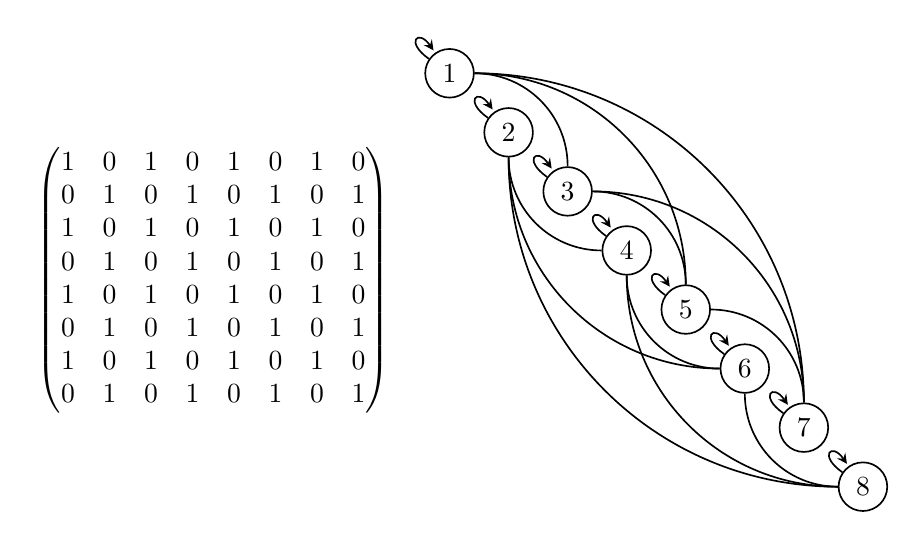
\begin{tikzpicture}[>=stealth, semithick, scale=0.75]
        \node (0) at (-4, 3.5) {
            \(\begin{pmatrix}
                1 & 0 & 1 & 0 & 1 & 0 & 1 & 0\\
                0 & 1 & 0 & 1 & 0 & 1 & 0 & 1\\
                1 & 0 & 1 & 0 & 1 & 0 & 1 & 0\\
                0 & 1 & 0 & 1 & 0 & 1 & 0 & 1\\
                1 & 0 & 1 & 0 & 1 & 0 & 1 & 0\\
                0 & 1 & 0 & 1 & 0 & 1 & 0 & 1\\
                1 & 0 & 1 & 0 & 1 & 0 & 1 & 0\\
                0 & 1 & 0 & 1 & 0 & 1 & 0 & 1
            \end{pmatrix}\)
        };
        \foreach \x in {1, 2, ..., 8} {
            \node[circle, draw] (\x) at (\x-1, 7-\x+1) {\x};
            \path[-] (\x) edge[in=125, out=145, loop] (\x);
        };
        \newcommand{\edgebendness}{45}
        \path[-] (1) edge[bend left=\edgebendness] (3) edge[bend left=\edgebendness] (5) edge[bend left=\edgebendness] (7);
        \path[-] (3) edge[bend left=\edgebendness] (5) edge[bend left=\edgebendness] (7);
        \path[-] (5) edge[bend left=\edgebendness] (7);
        \path[-] (8) edge[bend left=\edgebendness] (6) edge[bend left=\edgebendness] (4) edge[bend left=\edgebendness] (2);
        \path[-] (6) edge[bend left=\edgebendness] (4) edge[bend left=\edgebendness] (2);
        \path[-] (4) edge[bend left=\edgebendness] (2);
    \end{tikzpicture}
    \caption{The described graph for the chess-pattern Hamiltonian \((\sum_{j=0}^{1}\sum_{k=0}^{1} \ket{j}\bra{k})^{\otimes 2} \otimes E_2\).}
    \label{hamiltonian_graph_coloring_method}
\end{figure}

\phantom{}

We further take the following theorem as given. It concerns the Hamiltonian simulation of a decomposable Hamiltonian.

\begin{theorem} \label{suzuki_integrators}
    Let a decomposed Hamiltonian \(H = \sum_{j=1}^m H_j \in \mathbb{C}^{n \times n}\) with Hamiltonians \(H_1, ..., H_m \in \mathbb{C}^{n \times n}\) be given. Define the \emph{Suzuki higher order integrators \(S_{2k}\) of order \(k \in \mathbb{N}_{\geq 1}\)} recursively via
    \begin{align}
        S_2(\lambda) \coloneqq \prod_{j=1}^m e^{H_j \lambda/2} \prod_{j=1}^m e^{H_{m-j+1} \lambda/2} \qquad S_{2k}(\lambda) \coloneqq S_{2(k-1)}(p_k\lambda)^2S_{2(k-1)}((1-4p_k)\lambda)S_{2(k-1)}(p_k\lambda)^2
    \end{align}
    where \(\lambda \in \mathbb{C}\), \(p_k \coloneqq 1/(4-4^{1/(2k-1)})\). We have
    \begin{align}
        \norm{\exp\left(\lambda H\right) - S_{2k}(\lambda/r)^r} \in \onot(|\lambda|^{2k+1}/r^{2k})
    \end{align}
    for \(r \in \mathbb{N}_{\geq 1}\).
\end{theorem}

Berry et al. \cite{Berry2005} cite this result from \cite{Suzuki_1990}. Precisely, their cited result in eq. (4) of the paper is an application of the form in the eqs. (40-42) from \cite[p. 4]{Suzuki_1990}. The paper itself builds up on several research results on quantum monte carlo simulations \cite[p. 1]{Suzuki_1990} and concerns general decompositions of exponential operators. In the case of Hamiltonian simulation, we let \(\lambda \coloneqq it\). Using this bound and the ideas for the decomposition mentioned, the authors then obtain the following result.

\begin{theorem} \label{sparse_hamiltonian_simulation}
    Using \Cref{suzuki_integrators} and \Cref{small_sparse_ham_decomp}, there is a quantum algorithm, that computes the Hamiltonian simulation of a \(s\)-sparse, \(s \in \mathbb{N}\), efficiently-row computable Hamiltonian \(H\) for a time \(t \in \mathbb{R}_{\geq 0}\) acting on \(n\) qubits in time
    \begin{align}
        \onot\left(n\log_2^*(n)^2s^4\norm{H}te^{2\sqrt{\ln(5)\ln(s^2\norm{H}t/\varepsilon)}}\right) = \tilde{\onot}(\log_2(N) s^4 t)
    \end{align}
    where we denote by \(\tilde{\onot}(\cdot)\) the runtime under negligence of the expression \(\log_2^*(n)^2\norm{H}e^{2\sqrt{\ln(5)\ln(s^2\norm{H}t/\varepsilon)}}\).
\end{theorem}

With the simplified expression for the runtime using the notation \(\tilde{\onot}(\cdot)\), we follow Harrow et al. \cite[pp. 5-6]{Harrow2008}.

\emph{Derivation.} We give a short derivation of this result from the results of the paper. In \cite[pp. 8-9]{Berry2005}, we have the algorithm runtime with auxiliary operations of
\begin{align}
    \onot(n\log_2^*(n)^2d^25^{2k}(d^2\tau)^{1 + 1/(2k)}/\varepsilon^{1/(2k)}) = \onot(n\log_2^*(n)^2d^4\tau5^{2k}(d^2\tau)^{1/(2k)}/\varepsilon^{1/(2k)})
\end{align}
with \(\tau \coloneqq \norm{H}t\) and \(d \coloneqq s\) from the notation of the paper. The parameter \(k \in \mathbb{N}\) can be chosen at will, it corresponds to the depth of the recursion of the Suzuki higher order integrators. To optimize \(k\), we consider the given minimum at \cite[pp. 1-2]{Berry2005}. To derive it, observe
\begin{align}
    5^{2k}(d^2\tau/\varepsilon)^{1/(2k)} = e^{2k\ln(5)+\ln(d^2\tau/\varepsilon)/(2k)} \label{hamsim_small_exponential_rewrite}
\end{align}
and let
\begin{align}
    f\colon \mathbb{R} \to \mathbb{R}, k \mapsto 2k\ln(5)+\ln(d^2\tau/\varepsilon)/(2k)
\end{align}
reusing the symbol \(k\). Then we have
\begin{align}
    f'(k) = 2\ln(5) - \frac{\ln(d^2\tau/\varepsilon)}{2k^2}, f''(k) = \frac{\ln(d^2\tau/\varepsilon)}{k^3}
\end{align}
Solving for a minimum and using \(\log_5(x) = \ln(x)/\ln(5)\) for any \(x \in \mathbb{R}_{> 0}\) thus gives
\begin{align}
    k \approx \sqrt{\frac{\ln(d^2\tau/\varepsilon)}{4\ln(5)}} = \frac{1}{2}\sqrt{\log_5(d^2\tau/\varepsilon)}
\end{align}
Plugging this into \Cref{hamsim_small_exponential_rewrite} then gives the value
\begin{align}
    e^{\ln(5)\sqrt{\log_5(d^2\tau/\varepsilon)} + \sqrt{\ln(5)}\sqrt{\ln(d^2\tau/\varepsilon)}} = e^{2\sqrt{\ln(5)\ln(d^2\tau/\varepsilon)}}
\end{align}
So the runtime is
\begin{align}
    \onot\left(n\log_2^*(n)^2s^4\norm{H}te^{2\sqrt{\ln(5)\ln(s^2\norm{H}t/\varepsilon)}}\right)
\end{align}

\begin{remark}
    The contribution of keeping the error gap to the runtime is sublinear, meaning, that \(e^{2\sqrt{\ln(5)\ln(s^2\norm{H}t/\varepsilon)}} \in o(1/\varepsilon)\). Consider for that, that in general \(e^{2\sqrt{\ln(1/\varepsilon)}} \in o(1/\varepsilon)\), as \(\lim_{\varepsilon \to \infty} e^{2\sqrt{\varepsilon}}/\varepsilon = \lim_{\varepsilon \to \infty} e^{2\sqrt{\varepsilon}(1 - (1/2)\sqrt{\varepsilon})} \to 0\). The error contribution to the runtime thus may be neglected.
\end{remark}

\phantom{}

With this result, we may also introduce another auxiliary gate, taken from \cite[pp. 3-4]{Harrow2008}.

\begin{definition} \label{conditional_hamiltonian_evolution}
    The \emph{conditional Hamiltonian evolution} gate for some Hermitian \(A \in \mathbb{C}^{N \times N}, T \coloneqq 2^t, t \in \mathbb{N}_{\geq 1}, N \coloneqq 2^n\) and \(t_0 \in \mathbb{R}_{> 0}\) is the unitary map:
    \begin{align}
        \che_{T, N, A, t_0}\colon \mathbb{C}^{TN} \to \mathbb{C}^{TN}, \ket{x}\ket{y} \mapsto \left(\sum_{\tau = 0}^{T-1}\ket{\tau}\bra{\tau} \otimes e^{iA \tau t_0/T}\right) \ket{x}\ket{y}
    \end{align}
    \begin{align}
        \che_{T, N, A, t_0} = \begin{pmatrix}
            e^{iA \cdot 0 \cdot t_0/T} & 0 & \hdots & 0\\
            0 & e^{iA \cdot 1 \cdot t_0/T} & \hdots & 0\\
            \vdots & \vdots & \ddots & \vdots\\
            0 & 0 & \hdots & e^{iA \cdot (T-1) \cdot t_0/T}
        \end{pmatrix}
    \end{align}
\end{definition}

With this way of writing out the matrix for the conditional Hamiltonian evolution, it also becomes clear that it is unitary, as we can use \Cref{matrix_exponential_properties} and simulate the evolution for each \(k \in [0, N-1]_{\mathbb{N}}\)th of the \(n\) qubits individually using \(A\) with time \(t_0 k/T\), and thus a valid quantum gate.

\begin{remark}
    We will regard the runtime of the controlled Hamiltonian evolution to be the same as the individual Hamiltonian simulation, as in \Cref{sparse_hamiltonian_simulation}.
\end{remark}

    \section{The HHL Algorithm} \label{the_hhl_algorithm}

The currently asymptotically best classical method known for solving SLEs is the conjugate gradient method, which runs in worst case time \(\onot(N s \sqrt{\kappa} \log_2(1/\varepsilon))\), as described in \cite[complexity analysis on pp. 37-38]{Richard1994} or \cite[pp. 279-306]{Lyche}. Here, \(\varepsilon \in \mathbb{R}_{> 0}\) is the error cap, \(\kappa \in \mathbb{R}_{\geq 1}\) the condition number of the input \(N \times N\) matrix, where \(N \in \mathbb{N}_{\geq 1}\), and \(s \in \mathbb{N}\) is the sparsity as in \Cref{sparse_and_efficiently_row_computable_matrices}, assuming that the matrix is efficiently row-computable. In many practical cases, the given matrix has about \(\onot(\sqrt{N})\) non-zero entries, for which the algorithm yields a runtime of about \(\onot(N^{3/2} \sqrt{\kappa})\), ignoring the complexity factor for keeping the error low. In 2008, the researchers Harrow, Hassidim and Lloyd (HHL) described a quantum algorithmic approach to solving SLEs. In this section, we will give a rigorous description of the HHL algorithm, along with a rework of the original analysis. The original formulation can be found in \cite{Harrow2008}. We will draw a lot of information from the alternative, more comprehensive formulation presented by Dervovic et al. in \cite[pp. 28-42]{Dervovic2018} as well. Our contribution lies in the explicit description of the auxiliary procedures, such as the initialization of a helper state and a description on three-dimensional rotations, as well as more explicit runtime and error bounds. Most of these helper algorithms have been elaborated in \Cref{extensions_of_the_common_quantum_algorithmic_toolbox}.

\subsection{Problem Description and Assumptions \draftcommentgreen{DONE}} \label{hhl_problem_description_and_assumptions}

Starting off, let us pay attention to the general problem of solving SLEs.
\begin{problem}
    Given \(A \in \mathbb{C}^{m \times n}, b \in \mathbb{C}^m\) with \(m, n \in \mathbb{N}_{\geq 1}\), find an \(x \in \mathbb{C}^n\) with \(Ax = b\), if it exists.
\end{problem}
The HHL algorithm, in its original formulation, has the following requirements:
\begin{enumerate}
    \item \(m = n\) and \(n\) is a power of two.
    \item \(\norm{b} = 1\), so we may write \(\ket{b}\).
    \item \(\ket{b}\) can be initialized efficiently in a \(\log_2(n)\)-qubit register.
    \item \(A\) is well-conditioned, as in \Cref{well_conditioned_matrices}.
    \item The condition number \(\kappa(A) \in \mathbb{R}_{\geq 1}\), using the notation from \Cref{condition_number}, or at least an upper bound of it, must be known in advance.
\end{enumerate}
The result is then stored in a \(\log_2(n)\)-qubit register. So we may reformulate the problem.
\begin{problem} \label{hhl_problem}
    Given a well-conditioned \(A \in \mathbb{C}^{N \times N}\) with condition number \(\kappa \coloneqq \kappa(A) \in \mathbb{R}_{\geq 1}\) and an efficiently initializable state \(\ket{b} \in \mathbb{C}^N\), \(N \coloneqq 2^n\) and \(n \in \mathbb{N}_{\geq 1}\), find or approximate a quantum state \(\ket{x} \in \mathbb{C}^N\), s.t. there is a \(C \in (0, \infty)\) with \(A(C\ket{x}) = \ket{b}\).
\end{problem}
Note, that \(A\) may not be isometric, so we require that \(\ket{x}\) solves the inversion problem up to some positive multiplicative constant, which we can recover by comparing two non-zero elements of the vectors \(A\ket{x}\) and \(\ket{b}\). In \Cref{hhl_discussion}, we will discuss some techniques for relaxing the assumptions.

\subsection{Overview \draftcommentgreen{DONE}}

We carry over the notation introduced in \Cref{hhl_problem}. Let furthermore \(s \in \mathbb{N}\) be the sparsity of \(A\) and let \(\kappa \coloneqq \kappa(A)\). In total, we will require \(t+n+1\) qubits, where \(t \in \mathbb{N}_{\geq 5}\) is a hyperparameter. Let \(T \coloneqq 2^t\). One will need to choose \(t\) appropriately for the matrix \(A\), as described in the second next paragraph. In Dervovic et al., the first register is called the \emph{clock} register, the second the \emph{input} register and the third is an auxiliary qutrit \cite[p. 30]{Dervovic2018}. For the following, let \(\{(\lambda_1, \ket{v_1}), ..., (\lambda_N, \ket{v_N})\} \subseteq \left[\frac{1}{\kappa}, 1\right] \times \mathbb{C}^N\) be the eigenvalue-eigenvector pairs of an eigenbasis of \(A\) and decompose \(\ket{b}\) as
\begin{align}
    \ket{b} \eqqcolon \sum_{j=1}^N \beta_j \ket{v_j} = \sum_{j=1}^N \braket{b}{v_j} \ket{v_j}
\end{align}

\paragraph*{Brief Sketch of the Algorithm} \phantom{}\\\phantom{}

We now give a brief sketch of the algorithm. Following the decomposition of \(\ket{b}\) and \Cref{corollary_inverse_spectral_decomposition}, the aim is to approximate the quantum state
\begin{align}
    \ket{x} = \frac{1}{C} \sum_{j=1}^N \frac{\beta_j}{\lambda_j} \ket{v_j} \label{hhl_target_state}
\end{align}
with some \(C \in \mathbb{R}_{> 0}\). The algorithm starts in the state \(\ket{0}\ket{0}\ket{0} \in \mathbb{C}^{T N \cdot 3}\). The first steps are aimed towards approximating all eigenvalues of \(A\) simultaneously from all \(T\) possible canonical state vectors for the first register. To be precise, a state of form
\begin{align}
    \sum_{j=1}^N \beta_j \ket*{\tlj}\ket{v_j}\ket{0}
\end{align}
is first produced. \(\tlj\) here represents an approximation of \(\lambda_j\), s.t. \(|\lambda_j - \tlj| < \frac{2 \pi}{t_0}\), where \(t_0 \in \mathbb{R}_{> 0}\) is later chosen to minimize the overall error, but it is a large value in general. Such an approximation exists, if \(t\) and \(t_0\) are chosen well. The qutrit is then rotated to yield the state
\begin{align}
    \sum_{j=1}^N \beta_j \ket*{\tlj}\ket{v_j}\left(\sqrt{1-f^2(\tlj)-g^2(\tlj)}\ket{0}+f(\tlj)\ket{1}+g(\tlj)\ket{2}\right)
\end{align}
The functions \(f\colon \mathbb{R}_{> 0} \to [0, 1]\), \(g\colon \mathbb{R}_{> 0} \to [0, 1]\) are so-called \emph{filter functions} and defined in a way that allows filtering out tiny eigenvalues, such that taking their reciprocal does not produce an inaccurate state. With the assumptions made in \Cref{hhl_problem_description_and_assumptions}, \(g(\tlj) \approx 0\) and the filter functions thus evaluate to approximately give the state
\begin{align}
    \sum_{j=1}^N \beta_j \ket*{\tlj}\ket{v_j}\left(\sqrt{1-\frac{1}{4\kappa^2\tlj^2}}\ket{0}+\frac{1}{2\kappa\tlj}\ket{1}\right)
\end{align}
Uncomputing the eigenvalue approximation in the first register and applying amplitude amplification, as in \Cref{amplitude_amplification}, to measure a \(1\) in the qutrit gives us the state
\begin{align}
    \frac{1}{\sqrt{\frac{1}{4\kappa^2} \sum_{j = 1}^N \frac{|\beta_j|^2}{\tilde{\lambda_j^2}}}} \frac{1}{2\kappa} \sum_{j = 1}^N \frac{\beta_j}{\tlj} \ket{v_j}
\end{align}
in the second register, which corresponds to our target state as in \Cref{hhl_target_state}.

\paragraph*{Description of the Entire Algorithm} \phantom{}\\\phantom{}

We now give a full description of the HHL algorithm with an associated circuit diagram. The choice of the parameters \(\varepsilon\), \(t_0\) and \(t\) will be explained in the analysis of the algorithm.

{\centering\begin{minipage}{\linewidth}
    \vspace{-0.25cm}
    \begin{algorithm}[H]
        \caption{\textsc{HHL Algorithm}}
        \label{hhl_algorithm}
        \begin{algorithmic}[1]
            \Require A well-conditioned \(A \in \mathbb{C}^{N \times N}\) with condition number \(\kappa \in \mathbb{R}_{\geq 1}\) or an upper bound of it, where \(N \coloneqq 2^n\) with \(n \in \mathbb{N}_{\geq 1}\), a vector \(\ket{b} \in \mathbb{C}^N\), an efficiently implementable unitary \(\mathcal{B} \in \mathbb{C}^{N \times N}\) with \(\mathcal{B}\ket{0} = \ket{b}\) and an error cap \(\varepsilon \in \left(0, \frac{100}{4\pi}\right)\).
            \Ensure A quantum state \(\ket{\tilde{x}} \in \mathbb{C}^N\) with \(\norm{\ket{x}-\ket{\tilde{x}}} \leq \varepsilon\), where \(\ket{x}\) corresponds to the normalization of a vector \(x \in \mathbb{C}^N\) with \(Ax=\ket{b}\).
            \State Let \(t_0 \coloneqq 200\frac{\kappa}{\varepsilon}\) and \(t \coloneqq \max\{\lceil \log_2(t_0/2\pi) + 1 \rceil, 5\}\).
            \State \(\ket{\Psi} \coloneqq \ket{0}\ket{0}\ket{0} \in \mathbb{C}^{TN \cdot 3}\) empty \(t+n\) qubit-register with an ancilla qutrit.
            \State \(\ket{\Psi} \gets (\mathcal{T} \otimes \mathcal{B} \otimes E_3)\ket{\Psi}\)
            \State \(\ket{\Psi} \gets (\che_{T, N, A, t_0} \otimes E_3)\ket{\Psi}\)
            \State \(\ket{\Psi} \gets (\qft^\dagger_T \otimes E_{T \cdot 3}) \ket{\Psi}\)
            \State \(\ket{\Psi} \gets \mathcal{R}\ket{\Psi}\) with \(\mathcal{R}\) as defined below.
            \State \(\ket{\Psi} \gets (\qft_T \otimes E_{T \cdot 3})\ket{\Psi}\)
            \State \(\ket{\Psi} \gets (\che^\dagger_{T, N, A, t_0} \otimes E_3)\ket{\Psi}\)
            \State \(\ket{\Psi} \gets (\mathcal{T}^\dagger \otimes E_{N \cdot 3})\ket{\Psi}\)
            \State Perform amplitude amplification using \Cref{amplitude_amplification} on the previous steps to measure a \(1\) for the state \(\ket{\Psi}\) obtained from the previous steps with the function \(\chi\colon \{0, 1\}^{TN \cdot 3} \to \{0, 1\}\), s.t. \(\chi(x, y, z) = 1\), iff \(z = 1\) for any \(x \in [0, T-1]_{\mathbb{N}}\) and \(y \in [0, N-1]_{\mathbb{N}}\).
            \State \Return the \(n\)-qubit register of \(\ket{\Psi}\).
        \end{algorithmic}
    \end{algorithm}
\end{minipage}\par}

\phantom{}

The unitaries \(\mathcal{T} \in \mathbb{C}^{T \times T}\) and \(\mathcal{B} \in \mathbb{C}^{N \times N}\) are characterized by the following actions on \(\ket{0}\):
\begin{align}
    \mathcal{T}\ket{0} = \sqrt{\frac{2}{T}}\sum_{\tau = 0}^{T-1}\sin\left(\frac{\pi\left(\tau+\frac{1}{2}\right)}{T}\right)\ket{\tau} \qquad \mathcal{B}\ket{0} = \ket{b} \label{hhl_helper_init_proc_conditions}
\end{align}
We give a more detailled description and the implementation of \(\mathcal{T}\) further below. Furthermore, the so-called \emph{filter functions} \(f, g\colon \mathbb{R}_{\geq 0} \to \left[0, \frac{1}{2}\right]\) and their associated qutrit rotation unitary shall be defined as
\begin{align}
    f_{\kappa}(\lambda) &\coloneqq \begin{cases}
        0 & \lambda < \frac{1}{2\kappa}\\
        \frac{1}{2}\sin\left(\frac{\pi}{2} \cdot \frac{\lambda-\frac{1}{2\kappa}}{\frac{1}{\kappa}-\frac{1}{2\kappa}}\right) & \frac{1}{2\kappa} \leq \lambda < \frac{1}{\kappa}\\
        \frac{1}{2\kappa\lambda} & \frac{1}{\kappa} \leq \lambda
    \end{cases} \qquad g_{\kappa}(\lambda) \coloneqq \begin{cases}
        \frac{1}{2} & \lambda < \frac{1}{2\kappa}\\
        \frac{1}{2}\cos\left(\frac{\pi}{2} \cdot \frac{\lambda-\frac{1}{2\kappa}}{\frac{1}{\kappa}-\frac{1}{2\kappa}}\right) & \frac{1}{2\kappa} \leq \lambda < \frac{1}{\kappa}\\
        0 & \frac{1}{\kappa} \leq \lambda
    \end{cases} \label{filter_functions}\\
    \mathcal{R} &\coloneqq \sum_{\theta = 0}^{T-1} \ket{\theta}\bra{\theta} \otimes E_N \otimes R\left(\arcsin\left(\frac{f\left(\frac{2 \pi \theta}{t_0}\right)}{\sqrt{1-g^2\left(\frac{2 \pi \theta}{t_0}\right)}}\right), \arcsin(g\left(\frac{2 \pi \theta}{t_0}\right))\right)
\end{align}
where \(\mathcal{R}\) is constructed as in the proof of \Cref{qutrit_rotation}, here without additional helper qubits. Let furthermore \(f \coloneqq f_\kappa\) and \(g \coloneqq g_\kappa\), as \(\kappa\) is fixed.

\begin{figure}[!hbtp]
    \centering
    \begin{quantikz}
        \lstick{\(\ket{0}\)} \qw
        & \gate{\mathcal{T}} & \gate[wires=2]{\che_{T, N, A, t_0}}         & \gate{\qft^\dagger_T}             & \gate[wires=3]{\mathcal{R}}
        & \gate{\qft_T}      & \gate[wires=2]{\che_{T, N, A, t_0}^\dagger} & \gate{\mathcal{T}^\dagger} & \qw \rstick{\(\ket{0}\)}\\
        \lstick{\(\ket{0}\)} \qw
        & \gate{\mathcal{B}} & \qw & \qw  & \qw
        & \qw                & \qw & \qw & \qw \rstick{\(\ket{x}\)}\\
        \lstick{\(\ket{0}\)} \qw & \qw & \qw & \qw
        & \qw                    & \qw & \qw & \qw & \meter{1}
    \end{quantikz}
    \caption{Circuit diagram for the HHL algorithm. On the right, the register states for a perfect result are presented. We measure a \(1\), indicating a good result. We have not illustrated the amplitude amplification.}
    \label{hhl_algorithm_sketch}
\end{figure}

\paragraph*{Initialization Procedures} \phantom{}\\\phantom{}

As explained, we require two procedures \(\mathcal{T}\) and \(\mathcal{B}\) to prepare the first two registers of \(t\) and \(n\) qubits respectively, which we will explain in this paragraph starting with \(\mathcal{T}\). At first sight, it is not obvious, that the condition in \Cref{hhl_helper_init_proc_conditions} results in a valid quantum state. We introduce the following lemma.
\begin{lemma} \label{some_trigonometry_lemma}
    For any \(x \in \mathbb{C}\) it holds that:
    \begin{align}
        \sin^2\left(\frac{x}{2}\right) = \frac{1-\cos(x)}{2}
    \end{align}
\end{lemma}
\begin{proof}
    We use \Cref{sine_and_cosine_addition_theorem} and \Cref{trigonometric_pythagoras} to obtain:
    \begin{align}
        \cos(2x) = \cos^2(x)-\sin^2(x) = 1-2\sin^2(x)
    \end{align}
    Solving after \(\sin^2(x)\) and substituting \(x\) for \(x/2\) yields the statement.
\end{proof}
The next lemma then confirms the claim from before.
\begin{lemma} \label{sine_distr_lemma}
    Let \(T \coloneqq 2^t\), \(t \in \mathbb{N}_{\geq 1}\) and \(\tau \in [0, T-1]_{\mathbb{N}}\). It holds, that
    \begin{align}
        \sum_{k = 0}^{\tau} \frac{2}{T} \sin^2\left(\frac{\pi(k+\frac{1}{2})}{T}\right) = \frac{1}{T}\left(\tau + 1 - \frac{\sin\left(2(\tau+1)\frac{\pi}{T}\right)}{2\sin\left(\frac{\pi}{T}\right)}\right)
    \end{align}
\end{lemma}
\begin{proof}
    We can use \Cref{aa_cosine_helper_sum_lemma} from \Cref{amplitude_amplification_section}. Consider for any \(k \in [0, \tau]_{\mathbb{N}}\), using \Cref{some_trigonometry_lemma}:
    \begin{align}
        \sin^2\left(\frac{\pi(k+\frac{1}{2})}{T}\right) = \sin^2\left((2k+1)\frac{\pi}{2T}\right) = \frac{1}{2} \left(1-\cos\left((2k+1)\frac{\pi}{T}\right)\right)
    \end{align}
    So
    \begin{align}
        \sum_{k = 0}^{\tau} \frac{2}{T} \sin^2\left(\frac{\pi(k+\frac{1}{2})}{T}\right) &= \frac{1}{T}\left(\tau + 1 - \sum_{k=0}^\tau \cos\left((2k+1)\frac{\pi}{T}\right)\right)\\
        &= \frac{1}{T}\left(\tau + 1 - \frac{\sin\left(2(\tau + 1)\frac{\pi}{T}\right)}{2\sin\left(\frac{\pi}{T}\right)}\right)
    \end{align}
    under the use of \Cref{aa_cosine_helper_sum_lemma}.
\end{proof}
Inserting \(\tau = T-1\) gives the claim, that \(\mathcal{T}\) gives a valid quantum state. This closed formula further gives the following claim.
\begin{theorem} \label{hhl_clock_initialization}
    The procedure \(\mathcal{T}\) can be implemented to run in time \(\onot(t)\) with arbitrary precision.
\end{theorem}
\begin{proof}
    We wish to give an antiderivative \(P\) of a probability density function \(p\colon [0, \pi] \mapsto [0, 1]\) with for any \(\tau \in [0, T-1]_{\mathbb{N}}\)
    \begin{align}
        \int_{x_L^{t, \tau}}^{x_R^{t, \tau}} p = \frac{2}{T} \sin^2\left(\frac{\pi(\tau + \frac{1}{2})}{T}\right) \label{initialization_probability_density_values}
    \end{align}
    where \(x_L^{t, \tau} \coloneqq \pi \frac{\tau}{T}, x_R^{t, \tau} \coloneqq \pi \frac{\tau+1}{T}\). Let
    \begin{align}
        P\colon [0, \pi] \to [0, 1], x \mapsto \int_0^x p
    \end{align}
    Then for any \(\tau \in [0, T-1]_{\mathbb{N}}\):
    \begin{align}
        P(x_R^{t, \tau}) = \int_0^{x_R^{t, \tau}} p = \sum_{k = 0}^{\tau} \frac{2}{T} \sin^2\left(\frac{\pi(k+\frac{1}{2})}{T}\right) = \frac{1}{T}\left(\tau + 1 - \frac{\sin\left(2(\tau+1)\frac{\pi}{T}\right)}{2\sin\left(\frac{\pi}{T}\right)}\right) \label{probability_integral_equation}
    \end{align}
    using \Cref{sine_distr_lemma}. Consider the equation \(x = \frac{\pi(\tau + 1)}{T}\), from which we get \(\tau = \frac{T}{\pi}x-1\) to substitute \(\tau\) in \Cref{probability_integral_equation}. Letting \(x\) be loose gives
    \begin{align}
        P(x) = \frac{1}{T}\left(\frac{T}{\pi}x-\frac{\sin(2x)}{2\sin\left(\frac{\pi}{T}\right)}\right)
    \end{align}
    from which we obtain, that \(p\) is efficiently integrable, as efficient approximations of the sine exist. The use of \Cref{qsg_using_efficient_integrable_probability_distributions} gives the claim.
\end{proof}

\begin{remark}
    The values of \Cref{initialization_probability_density_values} resemble the normal distribution, as \Cref{sketch_of_the_amplitudes} shows. Furthermore, \(p\) roughly resembles a sigmoidal function, as the cumulative sums of the values in \Cref{initialization_probability_density_values} show, as pictured in \Cref{sketch_of_the_cumulative_amplitude_sums}. Especially the first observation may give some insight into why these coefficients were chosen, although we have not yet made the connection to the error analysis.
\end{remark}

\begin{remark}
    The problem of recovering an efficiently integrable probability density function, or its associated integral function, from given definite integrals may be interesting for the general quantum algorithmic toolbox. The proof of \Cref{hhl_clock_initialization} performs such a task for a very specific example, where much trigonometric structure is indeed involved, but finding such simple expressions may be hard in general. Uncountably many functions may suffice for such a task and canonical continuous functions for such interpolation tasks exist, one may look at Lagrangian interpolation, see \cite[p. 192]{Fischer2017}, but it is still unclear, if canonical efficiently computable functions for such interpolations exist.
\end{remark}

\phantom{}

\begin{figure}[!hbtp]
    \centering
    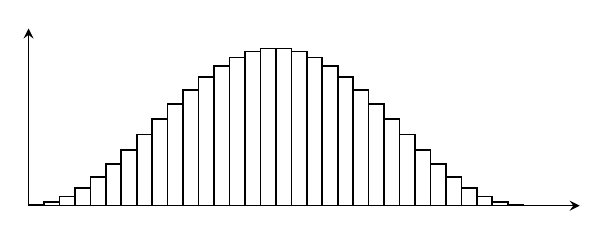
\begin{tikzpicture}[>=stealth, scale=2, semithick]
        \draw[->] (0, 0) -- (0, 1.125);
        \draw[->] (0, 0) -- (3.5, 0);
        \foreach \t in {0, 1, ..., 31} {
            \draw (pi * \t / 32, 0) rectangle ({pi * (\t + 1) / 32}, {16 * 2 / 32 * sin(180 / pi * pi * (\t + 0.5) / 32)^2});
        };
    \end{tikzpicture}
    \caption{Sketch of the amplitudes, here for \(t = 5\) and scaled by \(16\).}
    \label{sketch_of_the_amplitudes}
\end{figure}

\begin{figure}[!hbtp]
    \centering
    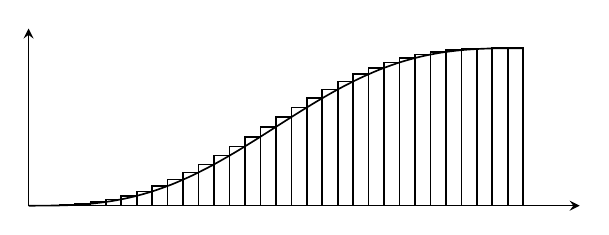
\begin{tikzpicture}[>=stealth, scale=2, semithick]
        \draw[->] (0, 0) -- (0, 1.125);
        \draw[->] (0, 0) -- (3.5, 0);
        \xdef\area{0};
        \foreach \t in {0, 1, ..., 31} {
            \pgfmathparse{\area + 2 / 32 * sin(180 / pi * pi * (\t + 0.5) / 32)^2};
            \xdef\area{\pgfmathresult};
            \draw (pi * \t / 32, 0) rectangle ({pi * (\t + 1) / 32}, {\area});
        };
        \draw[domain=0:3.1416, smooth] plot ({\x},  {1/32*(32/pi*\x-sin(deg(2*\x))/(2*sin(deg(pi/32))))});
    \end{tikzpicture}
    \caption{Sketch of the cumulative amplitude sums, here for \(t = 5\) and scaled by \(1\). The associated integral function of the probability distribution \(p\), \(P\), as found in the proof of \Cref{hhl_clock_initialization}, is also depicted.}
    \label{sketch_of_the_cumulative_amplitude_sums}
\end{figure}

As for the procedure \(\mathcal{B}\): We have discussed the problem of quantum state generation in \Cref{quantum_state_generation_based_on_efficiently_integrable_probability_distributions}. Efficient state generation is a key issue here, as an inefficient state generation procedure will drown the runtime of the HHL algorithm, as can be seen in \Cref{hhl_algorithm}.

\subsection{Analysis for Well-Conditioned Matrices \draftcommentgreen{DONE}}

We present the analysis from \cite{Harrow2008} with slightly different constants in the results. We assume, that none of the subprocedures produce an error, which one may consider to be a reasonable assumption due to our previous discussion on the complexity for keeping a low error gap for each subprocedure. Consider again the assumptions made in \Cref{hhl_problem_description_and_assumptions}.

\paragraph*{First Steps} \phantom{}\\\phantom{}

We first follow along the description of the algorithm in \Cref{hhl_algorithm} and observe the change of the registers. Initializing the first two registers yields
\begin{align}
    \ket{0}\ket{0}\ket{0} \xmapsto{\mathcal{T} \otimes \mathcal{B} \otimes E_3} \sqrt{\frac{2}{T}} \sum_{\tau = 0}^{T-1} \sin\left(\frac{\pi(\tau+\frac{1}{2})}{T}\right)\ket{\tau} \ket{b} \ket{0} = \sqrt{\frac{2}{T}} \sum_{j = 1}^N \beta_j \sum_{\tau = 0}^{T-1} \sin\left(\frac{\pi(\tau+\frac{1}{2})}{T}\right)\ket{\tau} \ket{v_j} \ket{0}
\end{align}
After that, applying \(\che_{T, N, A, t_0} \otimes E_3\) with effect on the first two registers and the use of \Cref{exponential_eigenvalue_theorem} gives
\begin{align}
    &\sqrt{\frac{2}{T}} \sum_{j = 1}^N \beta_j \sum_{\tau = 0}^{T-1} \sin\left(\frac{\pi(\tau+\frac{1}{2})}{T}\right)\che_{T, N, A, t_0} \ket{\tau} \ket{v_j} \ket{0}\\
    =& \sqrt{\frac{2}{T}} \sum_{j = 1}^N \beta_j \sum_{\tau = 0}^{T-1} \sin\left(\frac{\pi(\tau+\frac{1}{2})}{T}\right) e^{i \lambda_j \tau t_0 / T} \ket{\tau} \ket{v_j} \ket{0}
\end{align}
Now we apply \(\qft^\dagger_T \otimes E_{N \cdot 3}\), which, after some reordering, results in
\begin{align}
    &\sqrt{\frac{2}{T}} \sum_{j = 1}^N \beta_j \sum_{\tau = 0}^{T-1} \sin\left(\frac{\pi(\tau+\frac{1}{2})}{T}\right) e^{i \lambda_j \tau t_0 / T} \qft^\dagger_T \ket{\tau} \ket{v_j} \ket{0}\\
    =& \frac{\sqrt{2}}{T} \sum_{j = 1}^N \beta_j \sum_{\tau = 0}^{T-1} \sin\left(\frac{\pi(\tau+\frac{1}{2})}{T}\right) e^{i \lambda_j \tau t_0 / T} \sum_{k=0}^{T-1} e^{-2 \pi i k \tau / T} \ket{k} \ket{v_j} \ket{0}\\
    =& \frac{\sqrt{2}}{T} \sum_{j = 1}^N \beta_j \sum_{k = 0}^{T-1} \left(\sum_{\tau = 0}^{T-1} \sin\left(\frac{\pi(\tau+\frac{1}{2})}{T}\right) e^{\frac{i \tau}{T} (\lambda_j t_0 - 2 \pi k)}\right) \ket{k} \ket{v_j} \ket{0}\\
    \overset{\ref{hhl_first_steps_calc_1}}{=}& \sum_{j = 1}^N \beta_j \sum_{k = 0}^{T-1} \ajk \ket{k} \ket{v_j} \ket{0}
\end{align}

\begin{enumerate}[label=(\arabic*)]
    \item \label{hhl_first_steps_calc_1} Note that we define for these indices \(j, k\) the values \(\ajk \in \mathbb{C}\) and \(\djk \in \mathbb{R}\) via
    \begin{align}
        \ajk \coloneqq \frac{\sqrt{2}}{T} \sum_{\tau = 0}^{T-1} \sin\left(\frac{\pi(\tau+\frac{1}{2})}{T}\right) e^{\frac{i \tau}{T} \djk} \qquad \djk \coloneqq \lambda_j t_0 - 2 \pi k \label{ajk_djk_helpers}
    \end{align}
\end{enumerate}

This intermediate result corresponds to a ''good'' approximation of the eigenvalues of \(A\), as we will prove in the following paragraph. We only make one small observation.

\begin{observation} \label{basic_alpha_bound_and_alphas_are_prob_distr}
    We have \(\sum_{k=0}^{T-1} |\ajk|^2 = 1\). This follows by considering \(\ket{b} = \ket{v_j}\) and thus having
    \begin{align}
        \sum_{j=1}^N \beta_j \sum_{k=0}^{T-1} \ajk \ket{k}\ket{v_j}\ket{0} = \sum_{k=0}^{T-1} \ajk \ket{k}\ket{v_j}\ket{0}
    \end{align}
    be a valid quantum state with the \(\ajk\) values being independent of \(\beta_j\). Furthermore, we have \(|\ajk| \leq 1\).
\end{observation}

\begin{figure}[!hbtp]
    \centering
    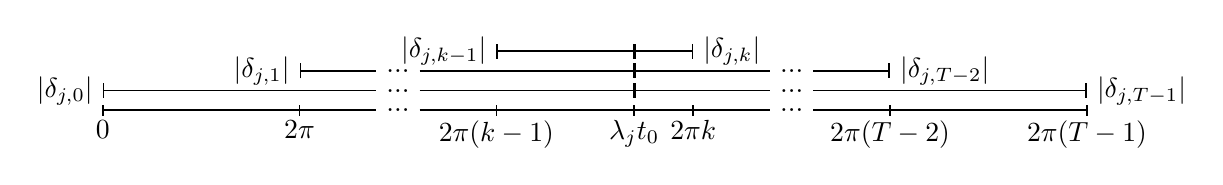
\begin{tikzpicture}[>=stealth, semithick]
        \newcommand{\dx}{2.5}
        \node[below] at (0*\dx, 0) {\(0\)};
        \node[below] at (1*\dx, 0) {\(2\pi\)};
        \draw (0*\dx, 0) -- (1*\dx, 0);
        \foreach \x in {0, 1, ..., 5}{
            \draw[shift={(\x*\dx, 0)}] (0, -2pt) -- (0, 2pt);
        };
        \node (0) at (1.5*\dx, 0) {...};
        \node (01) at (1.5*\dx, 0.25cm) {...};
        \node (02) at (1.5*\dx, 0.5cm) {...};
        \draw (1*\dx, 0) -- (0);
        \draw (0) -- (2*\dx, 0);
        \node[below] at (2*\dx, 0) {\(2\pi(k-1)\)};
        \node[below] at (3*\dx, 0) {\(2\pi k\)};
        \draw (2*\dx, 0) -- (3*\dx, 0);
        \node (1) at (3.5*\dx, 0) {...};
        \node (11) at (3.5*\dx, 0.25cm) {...};
        \node (12) at (3.5*\dx, 0.5cm) {...};
        \draw (3*\dx, 0) -- (1);
        \draw (1) -- (4*\dx, 0);
        \node[below] at (4*\dx, 0) {\(2\pi(T-2)\)};
        \node[below] at (5*\dx, 0) {\(2\pi(T-1)\)};
        \draw (4*\dx, 0) -- (5*\dx, 0);
        \draw[shift={(2.7*\dx, 0)}] (0, -2pt) -- (0, 2pt);
        \node[below] at (2.7*\dx, 0) {\(\lambda_j t_0\)};
        \draw[|-] (0*\dx, 0.25cm) -- (01) node[left, pos=0] {\(|\delta_{j, 0}|\)};
        \draw[-|] (01) -- (2.7*\dx, 0.25cm);
        \draw[|-] (1*\dx, 0.5cm) -- (02) node[left, pos=0] {\(|\delta_{j, 1}|\)};
        \draw[-|] (02) -- (2.7*\dx, 0.5cm);
        \draw[|-|] (2*\dx, 0.75cm) -- (2.7*\dx, 0.75cm) node[left, pos=0] {\(|\delta_{j, k-1}|\)};
        \draw[|-] (2.7*\dx, 0.25cm) -- (11);
        \draw[-|] (11) -- (5*\dx, 0.25cm) node[right] {\(|\delta_{j, T-1}|\)};
        \draw[|-] (2.7*\dx, 0.5cm) -- (12);
        \draw[-|] (12) -- (4*\dx, 0.5cm) node[right] {\(|\delta_{j, T-2}|\)};
        \draw[|-|] (2.7*\dx, 0.75cm) -- (3*\dx, 0.75cm) node[right, pos=1] {\(|\delta_{j, k}|\)};
    \end{tikzpicture}
    \caption{A line representing \([0, 2 \pi (T-1)]\) with marks for understanding the behavior of the approximations for one \(\djk\) value. We assume an appropriate choice for \(t\), as described in this text. In this case, the approximation seems to be of poor quality, increasing \(t\) will improve the accuracy as then the interval \([2\pi(k-1), 2\pi k]\) will be split in half and \(2\pi(2k-1)\) will give a better approximation.}
    \label{delta_values_visualized}
\end{figure}

\paragraph*{Analysis of the Phase Estimation} \label{hhl_phase_estimation_analysis} \phantom{}\\\phantom{}

The following analysis of the coefficients \(\ajk\) is based on the original HHL paper \cite[pp. 10-11]{Harrow2008} and Dervovic et al. \cite[pp. 32-33]{Dervovic2018}, but we do not fully agree with the assumptions used. Our goal is to prove, that for each \(j \in [1, N]_{\mathbb{N}}\), there are at most two values \(k \in [0, T-1]_{\mathbb{N}}\), where the coefficients \(\ajk\) concentrate at, meaning that the sum of their squared magnitudes is large in comparison to the magnitude sums of the exponentially many other approximations, and, such that \(2 \pi k / t_0\) is a good approximation of \(\lambda_j\). To get some intuition on this analysis, notice, that the value \(\djk\) becomes very small if \(2 \pi k / t_0 \approx \lambda_j\). We try to carry this intuition over to the coefficients \(\ajk\). The main result of this paragraph will be the following theorem.

\begin{theorem} \label{alphas_yield_good_approximation}
    For the HHL phase estimation of an eigenvalue \(\lambda_j\) with \(j \in [1, N]_{\mathbb{N}}\) arbitrary, but fixed, it holds, that
    \begin{align}
        \sum_{\substack{k \in [0, T-1]_{\mathbb{N}}\\|\djk| \geq 2\pi}} |\ajk|^2 < \frac{7}{10}
    \end{align}
\end{theorem}

Let \(j\), \(k\) as in \Cref{ajk_djk_helpers} be arbitrary, but fixed with \(|\djk| \geq 2\pi\).

\begin{observation} \label{inner_amplitude_bounds}
    By definition and \(\lambda_j \in \left[\frac{1}{\kappa}, 1\right]\), we have \(|\djk| \leq \max(\{t_0, 2 \pi (T-1)\})\). Since, due to the algorithm description, we assume a choice of \(t\), s.t. \(t_0 \leq 2 \pi (T-1)\), as \(T \geq t_0/2\pi+1\), we get
    \[
        2\pi \leq |\djk| \leq 2 \pi (T-1)
    \]
\end{observation}

We disagree with the assumption by the HHL authors, that \(|\delta_{i, j}| \leq T/10\) \cite[p. 11]{Harrow2008}. If one applies the algorithm on any unit matrix and chooses \(t_0\) to be incredibly high, whilst using only few helper qubits, the bound will not hold. In the following, we present a detailled derivation of the alternative representation of the \(\ajk\) values, which can be found in \cite[p. 11]{Harrow2008}.

\begin{restatable}{lemma}{sinebound} \label{sine_bound}
    The following bounds hold for any \(x \in \mathbb{R}_{\geq 0}\):
    \begin{align}
        x - \frac{x^3}{6} \leq \sin(x) \leq x
    \end{align}
    With strict inequalities for \(x \neq 0\).
\end{restatable}

The lower bound is not obvious. We present the proof of this rather elementary bound in \Cref{sine_bound_proof}.

\begin{lemma} \label{alpha_values_rewrite}
    The following statements hold.
    \begin{enumerate}[label=(\roman*)]
        \item[\ref{alpha_values_rewrite_1}] For \(\djk \notin \{\pm \pi\}\), it holds, that
        \begin{align}
            \ajk = -e^{i\frac{\djk}{2}\left(1-\frac{1}{T}\right)}\frac{\sqrt{2}\cos\left(\frac{\djk}{2}\right)}{T} \frac{\cos\left(\frac{\djk}{2T}\right)\sin\left(\frac{\pi}{2T}\right)}{\sin\left(\frac{\djk+\pi}{2T}\right)\sin\left(\frac{\djk-\pi}{2T}\right)}
        \end{align}
        \item[\ref{alpha_values_rewrite_2}] The function
        \begin{align}
            \xi \colon (-2\pi, 2\pi) \setminus \{\pm \pi\} \to \mathbb{R}, \delta \mapsto \frac{2}{T^2} \sin^2\left(\frac{\pi}{2T}\right) \frac{\cos^2\left(\frac{\delta}{2}\right)\cos^2\left(\frac{\delta}{2T}\right)}{\sin^2\left(\frac{\delta+\pi}{2T}\right)\sin^2\left(\frac{\delta-\pi}{2T}\right)}
        \end{align}
        can be continuously extended to \((-2\pi, 2\pi)\).
    \end{enumerate}
\end{lemma}

\begin{proof}
    \begin{enumerate}[label=(\roman*)]
        \item \label{alpha_values_rewrite_1} We give thorough explanations to the following large computation.
        \begin{align}
            \ajk &= \frac{\sqrt{2}}{T} \sum_{\tau = 0}^{T-1} \sin\left(\frac{\pi(\tau+\frac{1}{2})}{T}\right) \exp\left(\frac{i \tau}{T} \djk\right)\\
            &\overset{\ref{alpha_values_rewrite_step_1}}{=} \frac{1}{i\sqrt{2}T} \sum_{\tau = 0}^{T-1} \exp\left(\frac{i\tau}{T}\djk\right)\left(\exp\left(i\frac{\pi(\tau+\frac{1}{2})}{T}\right)-\exp\left(-i\frac{\pi(\tau+\frac{1}{2})}{T}\right)\right)\\
            &\overset{\ref{alpha_values_rewrite_step_2}}{=} \frac{1}{i\sqrt{2}T} \left(\exp\left(\frac{i\pi}{2T}\right)\sum_{\tau = 0}^{T-1}\exp\left(i\tau\frac{\djk+\pi}{T}\right) - \exp\left(-\frac{i\pi}{2T}\right)\sum_{\tau = 0}^{T-1}\exp\left(i\tau\frac{\djk-\pi}{T}\right)\right)\\
            &\overset{\ref{alpha_values_rewrite_step_3}}{=} \frac{1}{i\sqrt{2}T} \left(\exp\left(\frac{i\pi}{2T}\right)\frac{1-e^{i(\djk+\pi)}}{1-e^{i\frac{\djk+\pi}{T}}} - \exp\left(-\frac{i\pi}{2T}\right)\frac{1-e^{i(\djk-\pi)}}{1-e^{i\frac{\djk-\pi}{T}}}\right) \label{special_djk_bounds}\\
            &\overset{\ref{alpha_values_rewrite_step_4}}{=} \frac{1+e^{i\djk}}{i\sqrt{2}T} \left(\frac{e^{-i\frac{\djk}{2T}}}{e^{-i\frac{\djk+\pi}{2T}}-e^{i\frac{\djk+\pi}{2T}}} - \frac{e^{-i\frac{\djk}{2T}}}{e^{-i\frac{\djk-\pi}{2T}}-e^{i\frac{\djk-\pi}{2T}}}\right)\\
            &\overset{\ref{alpha_values_rewrite_step_5}}{=} \frac{(1+e^{i\djk})e^{-i\frac{\djk}{2T}}}{i\sqrt{2}T} \left(\frac{1}{-2i\sin\left(\frac{\djk+\pi}{2T}\right)} - \frac{1}{-2i\sin\left(\frac{\djk-\pi}{2T}\right)}\right)\\
            &\overset{\ref{alpha_values_rewrite_step_6}}{=} e^{i\frac{\djk}{2}\left(1-\frac{1}{T}\right)}\frac{\cos\left(\frac{\djk}{2}\right)}{\sqrt{2}T} \frac{\sin\left(\frac{\djk-\pi}{2T}\right)-\sin\left(\frac{\djk+\pi}{2T}\right)}{\sin\left(\frac{\djk+\pi}{2T}\right)\sin\left(\frac{\djk-\pi}{2T}\right)}\\
            &\overset{\ref{alpha_values_rewrite_step_7}}{=} -e^{i\frac{\djk}{2}\left(1-\frac{1}{T}\right)}\frac{\sqrt{2}\cos\left(\frac{\djk}{2}\right)}{T} \frac{\cos\left(\frac{\djk}{2T}\right)\sin\left(\frac{\pi}{2T}\right)}{\sin\left(\frac{\djk+\pi}{2T}\right)\sin\left(\frac{\djk-\pi}{2T}\right)}
        \end{align}
    
        \begin{enumerate}[label=(\arabic*), wide]
            \item \label{alpha_values_rewrite_step_1} Use the definition of the sine with the complex exponential function, see \Cref{exponential_sine_and_cosine}.
            \item \label{alpha_values_rewrite_step_2} Reorder the terms wrt. the dependency on \(\tau\).
            \item \label{alpha_values_rewrite_step_3} Use the geometric sum. With \(\djk \notin \{\pm \pi\}\), it is assured, that we do not add up ones, as otherwise the geometric sum does not apply here in this form.
            \item \label{alpha_values_rewrite_step_4} Notice \(e^{i(\djk+\pi)} = -e^{i\djk} = e^{i(\djk-\pi)}\) by definition. Thus, we first factor out \(1+e^{i\djk}\). Expand the terms by \(e^{-i\frac{\djk+\pi}{2T}}\) and \(e^{-i\frac{\djk-\pi}{2T}}\), through which the factors \(e^{\frac{i\pi}{2T}}\) and \(e^{-\frac{i\pi}{2T}}\) get cancelled out.
            \item \label{alpha_values_rewrite_step_5} Factor out the numerators and use the definition of the sine via the complex exponential function, see \Cref{exponential_sine_and_cosine}, in the denominators.
            \item \label{alpha_values_rewrite_step_6} Factoring out \(1/(-2i)\) from the sums yields a denominator of \(2\sqrt{2}T\). Now, using the exponential form of the \emph{cosine} function for once, we also obtain:
            \begin{align}
                (1+e^{i\djk})e^{-i\frac{\djk}{2T}} = (e^{-i\frac{\djk}{2}}+e^{i\frac{\djk}{2}})e^{i\frac{\djk}{2}\left(1-\frac{1}{T}\right)} = 2\cos\left(\frac{\djk}{2}\right)e^{i\frac{\djk}{2}\left(1-\frac{1}{T}\right)}
            \end{align}
            At last, we expand the right terms. This fixes one calculation mistake of the original paper: The \(\sqrt{2}\) is part of the denominator.
            \item \label{alpha_values_rewrite_step_7} We use the sine addition theorem, see \Cref{sine_and_cosine_addition_theorem}. With the asymmetry of the sine function, and the symmetry of the cosine function, this yields:
            \begin{align}
                \sin\left(\frac{\djk-\pi}{2T}\right)-\sin\left(\frac{\djk+\pi}{2T}\right) &= \cos\left(\frac{\djk}{2T}\right)\sin\left(\frac{-\pi}{2T}\right)-\cos\left(\frac{\djk}{2T}\right)\sin\left(\frac{\pi}{2T}\right)\\
                &= -2\cos\left(\frac{\djk}{2T}\right)\sin\left(\frac{\pi}{2T}\right)
            \end{align}
        \end{enumerate}
        \item \label{alpha_values_rewrite_2} Notice \(\xi(-\delta) = \xi(\delta)\) due to \(\sin^2\left(\frac{-\delta+\pi}{2T}\right)\sin^2\left(\frac{-\delta-\pi}{2T}\right) = \sin^2\left(\frac{\delta+\pi}{2T}\right)\sin^2\left(\frac{\delta-\pi}{2T}\right)\) and the axial symmetry of the cosine. It thus suffices to prove the existence of \(\lim_{\delta \to \pi} \xi(\delta)\). We have
        \begin{align}
            \lim_{\delta \to \pi} \frac{\cos\left(\frac{\delta}{2}\right)\cos\left(\frac{\delta}{2T}\right)}{\sin\left(\frac{\delta+\pi}{2T}\right)\sin\left(\frac{\delta-\pi}{2T}\right)} = \frac{\evalat{\frac{\partial}{\partial \delta} \cos\left(\frac{\delta}{2}\right)\cos\left(\frac{\delta}{2T}\right)}{\pi}}{\frac{1}{2T}\sin\left(\frac{\pi}{T}\right)}
        \end{align}
        using the rule of Bernoulli-L'Hospital \cite[pp. 150-151]{Koenigsberger2003} and
        \begin{align}
            \frac{\partial}{\partial \delta} \sin\left(\frac{\delta+\pi}{2T}\right)\sin\left(\frac{\delta-\pi}{2T}\right) &= \frac{1}{2T}\left(\cos\left(\frac{\delta+\pi}{2T}\right)\sin\left(\frac{\delta-\pi}{2T}\right)+\sin\left(\frac{\delta+\pi}{2T}\right)\cos\left(\frac{\delta-\pi}{2T}\right)\right)\\
            &= \frac{1}{2T}\sin\left(\frac{\delta}{T}\right)
        \end{align}
        using the product rule of differential calculus and \Cref{sine_and_cosine_addition_theorem}. Taking the continuity of \(\delta \mapsto \delta^2\) into account, we obtain the statement.
    \end{enumerate}

    This concludes the proof.
\end{proof}

Part \ref{alpha_values_rewrite_2} of this lemma will not be used, its importance lies in the fact, that the \(\ajk\) values do not ''blow up'' for values \(|\djk|\) near \(\pi\). We now present a descriptive analytic proof for the bound concentration, i.e., that for \(j\) and \(k\) with \(|\djk| < 2\pi\), we have a good approximation of \(\lambda_j\) by \(\frac{2 \pi k}{t_0}\). It holds, that
\begin{align}
    |\ajk| \overset{\ref{small_ajk_calc_1}}{=} \frac{\sqrt{2}\left|\cos\left(\frac{\djk}{2}\right)\right|}{T} \frac{\left|\cos\left(\frac{\djk}{2T}\right)\right|\sin\left(\frac{\pi}{2T}\right)}{\sin\left(\frac{\djk+\pi}{2T}\right)\sin\left(\frac{\djk-\pi}{2T}\right)} \overset{\ref{small_ajk_calc_2}}{<} \frac{\pi}{\sqrt{2}T^2} \frac{1}{\sin\left(\frac{\djk+\pi}{2T}\right)\sin\left(\frac{\djk-\pi}{2T}\right)} \label{first_alpha_magnitude_rewrite}
\end{align}
\begin{enumerate}[label=(\arabic*), wide]
    \item \label{small_ajk_calc_1} Taking the complex magnitude respects products, \(\left|-\exp(i\frac{\djk}{2}\left(1-\frac{1}{T}\right))\right| = 1\) and  \(\frac{\pi}{2T} \in \left(0, \frac{\pi}{64}\right)\), where the sine is positive. Furthermore, for \(\djk > 0\), we have \(\frac{\djk+\pi}{2T}, \frac{\djk-\pi}{2T} \in \left[\frac{\pi}{2T}, \pi - \frac{\pi}{2T}\right]\), where the sine is also positive. We also have \(\sin\left(\frac{-\djk+\pi}{2T}\right)\sin\left(\frac{-\djk-\pi}{2T}\right) = \sin\left(\frac{\djk-\pi}{2T}\right)\sin\left(\frac{\djk+\pi}{2T}\right)\), so we can leave out taking the magnitude again.
    \item \label{small_ajk_calc_2} Since \(|\cos| \leq 1\) with strict inequality for arguments outside of \(\pi \mathbb{Z}\), and \Cref{sine_bound}.
\end{enumerate}

We want to further study the result analytically.

\begin{lemma} \label{continuous_delta_alpha_behavior}
    Define the auxiliary function
    \begin{align}
        h\colon \mathbb{R} \setminus \{2 \pi k T \pm \pi \mid k \in \mathbb{Z}\} \to \mathbb{R}_{> 0}, \delta \mapsto \frac{\pi}{\sqrt{2}T^2} \frac{1}{\sin\left(\frac{\delta+\pi}{2T}\right)\sin\left(\frac{\delta-\pi}{2T}\right)}
    \end{align}
    and let \(h^\pm \coloneqq h|_{[\pm2\pi(T-1), \pm2\pi] \cup [\pm2\pi, \pm2\pi(T-1)]}\) each yielding \(h^+\) and \(h^-\). We have
    \begin{enumerate}[label=(\roman*)]
        \item \(h^-(-\delta) = h^+(\delta)\) for \(\delta \in [2\pi, 2\pi(T-1)]\).
        \item \(h^+\) is symmetric wrt. \(\pi T\).
        \item \(h^+|_{[2\pi, \pi T]}\) strictly descends.
    \end{enumerate}
\end{lemma}

\begin{proof}
    \begin{enumerate}[label=(\roman*)]
        \item We have proven this in \ref{small_ajk_calc_1} for \Cref{first_alpha_magnitude_rewrite}.
        \item If \(\delta \in [2\pi, \pi T]\), then \(2 \pi T - \delta \in [\pi T, 2\pi(T-1)]\). Especially
        \begin{align}
            \sin\left(\frac{(2 \pi T - \delta) + \pi}{2T}\right)\sin\left(\frac{(2 \pi T - \delta) - \pi}{2T}\right) &= \sin\left(\pi - \frac{\delta - \pi}{2T}\right)\sin\left(\pi - \frac{\delta + \pi}{2T}\right)\\
            &= \sin\left(\frac{\delta - \pi}{2T}\right)\sin\left(\frac{\delta + \pi}{2T}\right)
        \end{align}
        \item As \(\frac{\partial}{\partial \delta} \sin\left(\frac{\delta+\pi}{2T}\right)\sin\left(\frac{\delta-\pi}{2T}\right) = \frac{1}{2T} \sin\left(\frac{\delta}{T}\right) \geq 0\) in \([2\pi, \pi T]\), see \Cref{l_functions_derivatives_1}, the function stricly descends. Note, that the right bound does not matter by the definition of strict monotonicity.
    \end{enumerate}
\end{proof}

\begin{remark}
    The consequence of this lemma is, that we can reduce the calculation of \(h\) for any \(\djk\) by mirroring the value at most twice, once around \(x = 0\) and once around \(x = \pi T\). As the \(\djk\) values are evenly spread on an interval of length \(2\pi (T-2)\), we can further bound any sum over all \(\ajk\) values by only considering the values of \(h\) in \([2\pi, \pi (T-1)]\). We shall use this thought in the proof of \Cref{alphas_yield_good_approximation}.
\end{remark}

\begin{restatable}{lemma}{sinecomplemma} \label{sine_comp_lemma}
    Defining for \(T \coloneqq 2^t\), \(t \in \mathbb{N}_{\geq 5}\)
    \begin{align}
        l^\uparrow\colon [2\pi, \pi T] \to \mathbb{R}, \delta \mapsto \sin\left(\frac{\delta + \pi}{2T}\right)\sin\left(\frac{\delta - \pi}{2T}\right) \qquad l^\downarrow\colon [2\pi, \pi T] \to \mathbb{R}, \delta \mapsto \frac{c_1}{\pi^2} \frac{\delta^2}{T^2}
    \end{align}
    where \(c_1 \coloneqq 0.9975 < \sin\left(\frac{\pi}{2}-\frac{\pi}{64}\right)\), we have \(l^\uparrow > l^\downarrow\).
\end{restatable}

We leave out the technicalities of this lemma and prove it in the appendix, see \Cref{sine_comp_lemma_proof}. Consider the illustration with a summary of the argument in \Cref{sine_comp_lemma_visualized}.

\begin{figure}[!hbtp]
    \centering
    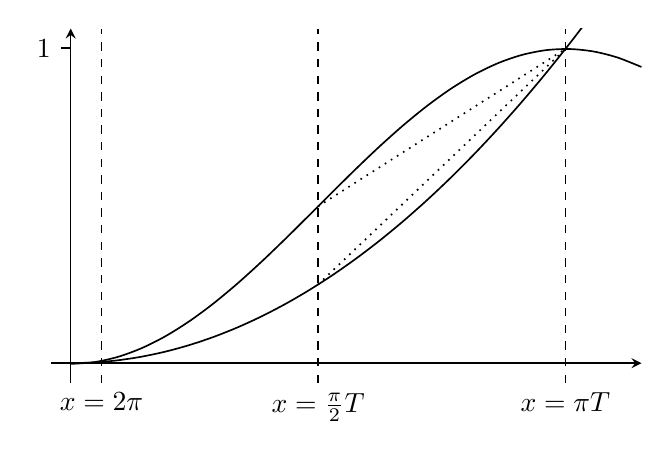
\begin{tikzpicture}[>=stealth, scale=2, semithick]
        \draw[->] (-0.125, 0) -- (3.625, 0);
        \draw[->] (0, -0.125) -- (0, 2.125);

        \draw (-0.0625, 2) -- (0, 2) node[left, pos=0] {\(1\)};
        \draw[dashed] (0.1963, -0.125) -- (0.1963, 2.125) node[below, pos=0] {\(x = 2\pi\)};
        \draw[dashed] (1.5710, -0.125) -- (1.5710, 2.125) node[below, pos=0] {\(x = \frac{\pi}{2}T\)};
        \draw[dashed] (3.1416, -0.125) -- (3.1416, 2.125) node[below, pos=0] {\(x = \pi T\)};

        \clip (-0.125, -0.125) rectangle (3.625, 2.125);
        \draw[domain=0:3.625, range=0:2, smooth] plot ({\x},  {2 * sin(deg((\x*32+pi)/64)) * sin(deg((\x*32-pi)/64))});
        \draw[domain=0:3.625, range=0:2, smooth] plot ({\x},  {2 * 0.9975/(pi^2) * (\x^2*32^2)/(32^2)});
        \draw[dotted] (1.5710, 2 * 0.4976) -- (3.1416, 2 * 0.9976);
        \draw[dotted] (1.5710, 2 * 0.2494) -- (3.1416, 2 * 0.9975);
    \end{tikzpicture}
    \caption{Graph of \(l^\uparrow\) and \(l^\downarrow\) für \(t = 5\). The \(x\)-axis is scaled by \(1/T\), the \(y\)-axis is scaled by \(2\) and the entire plot is scaled by 2. The vertical lines \(x = 2\pi\), \(x = \frac{\pi}{2} T\) and \(x = \pi T\) are marked. In the interval \([2\pi, \pi T/2]\), \(l^\uparrow\) grows faster than \(l^\downarrow\), while being larger at the interval boundaries. In \([\pi T / 2, \pi T]\), \(l^\uparrow\) is convex, and larger at the boundary points, while \(l^\downarrow\) is concave. The convexity and concavity argument is illustrated by the dotted lines. These facts conclude \(l^\uparrow > l^\downarrow\). The rigorous formulation can be found in the appendix, as said.}
    \label{sine_comp_lemma_visualized}
\end{figure}

\begin{lemma} \label{alpha_delta_values_relation}
    For \(2\pi \leq \djk \leq \pi T\), we have
    \begin{align}
        |\ajk| < \frac{22}{\djk^2}
    \end{align}
\end{lemma}

\begin{proof}
    \Cref{sine_comp_lemma} and \Cref{alpha_values_rewrite} directly give us
    \begin{align}
        |\ajk| < \frac{\pi}{\sqrt{2}T^2} \frac{\pi^2}{c_1} \frac{T^2}{\djk^2} < \frac{22}{\djk^2}
    \end{align}
\end{proof}

\begin{remark}
    For a guarantee of a good approximation of the eigenvalues, \Cref{helper_qubits_needed} shows, that at least five qubits are needed.
\end{remark}

Now we are able to give the proof of the main theorem of this subsection.

\begin{proof}[Proof of \Cref{alphas_yield_good_approximation}]
    Due to the behavior of \(h\) in \Cref{continuous_delta_alpha_behavior}, we have
    \begin{align}
        \sum_{\substack{k \in [0, T-1]_{\mathbb{N}}\\|\djk| \geq 2\pi}} |\ajk|^2 \overset{\ref{continuous_delta_alpha_behavior_1}}{<} \sum_{k=1}^{T-1} h(2 \pi k)^2 \overset{\ref{continuous_delta_alpha_behavior_2}}{<} 2\sum_{k=1}^\infty \frac{22^2}{16\pi^4k^4} \overset{\ref{continuous_delta_alpha_behavior_3}}{=} 2 \cdot \frac{22^2}{16 \cdot 90} < \frac{7}{10}
    \end{align}
    \begin{enumerate}[label=(\arabic*), wide]
        \item \label{continuous_delta_alpha_behavior_1} The values \(\djk\) are positioned in distance \(2\pi\) to each closest neighbor. Consider for each \(k\), that \(|\djk| \in [2 \pi k', 2 \pi (k'+1)]\) for some \(k' \in \mathbb{Z}\). With the monotonicity behavior of \(h\), as in \Cref{continuous_delta_alpha_behavior}, we thus have the upper bound using \(h^2\) at either \(2 \pi k'\) or \(2 \pi (k'+1)\) for this value \(|\ajk|^2\). To observe the statement for the sum, consider for a \(k\) with \(\djk < 0\), that mirroring, i.e. taking \(h^2(-\djk)\) for the strict upper bound, and then mirroring at \(\pi T\), gives the upper bound, and that no other element is then contained in the associated \(2 \pi\)-sized interval, in which \(2 \pi T + \djk\) lies, as then we have \(\delta_{j, 0} - \delta_{j, T-1} > 2 \pi (T-1)\), which is a contradiction to the definition of the \(\djk\) values.
        \item \label{continuous_delta_alpha_behavior_2} Following our previous considerations, we upper bound the values for \(\djk \in [2\pi, \pi T]\) twice and let them tend to infinity for a constant upper bound.
        \item \label{continuous_delta_alpha_behavior_3} Using \Cref{zeta_two}.
    \end{enumerate}
\end{proof}

\begin{remark} \label{eigenvalue_approximations_notation}
    With the last theorem proven, we will now use the notation \(\ket*{\tlk} \coloneqq \ket{k}\), \(k \in [0, T-1]_{\mathbb{N}}\), following \cite[p. 6]{Harrow2008}, for the basis states, where \(\tlk \coloneqq \frac{2 \pi k}{t_0}\). Note that with this notation, we indicate that for some such \(k\), \(\tlk\) gives a good approximation for some eigenvalue \(\lambda_j\), \(j \in [1, N]_{\mathbb{N}}\).
\end{remark}

The following theorem further elaborates the existence of a close approximation.

\begin{theorem}[Existence of Eigenvalue Approximations] \label{existence_of_eigenvalue_approximations}
    The following statements hold for any fixed \(j \in [1, N]_{\mathbb{N}}\).
    \begin{enumerate}[label=(\roman*)]
        \item[\ref{existence_of_eigenvalue_approximations_1}] There is a \(k \in [0, T-1]_{\mathbb{N}}\) with \(|\djk| < 2\pi\).
        \item[\ref{existence_of_eigenvalue_approximations_2}] For every \(k \in [0, T-1]_{\mathbb{N}}\) with \(|\djk| < 2\pi\), we have
        \begin{align}
            |\tlk - \lambda_j| < \frac{1}{4\kappa}
        \end{align}
        and thus
        \begin{align}
            \tlk \in \left(\frac{3}{4\kappa}, 1 + \frac{1}{4\kappa}\right)
        \end{align}
    \end{enumerate}
\end{theorem}

\begin{proof} We prove the statements in series.

    \begin{enumerate}[label=(\roman*)]
        \item \label{existence_of_eigenvalue_approximations_1} Fix \(j\) and consider under the condition \(\djk \leq 0\)
        \begin{align}
            0 \leq -\djk = 2 \pi k - \lambda_jt_0 < 2\pi \leadsto \frac{\lambda_jt_0}{2\pi} < k < \frac{\lambda_jt_0}{2\pi}+1
        \end{align}
        as \(\frac{\lambda_jt_0}{2\pi} \in (0, T-1)\), we may thus choose \(k \coloneqq \left\lfloor \frac{\lambda_jt_0}{2\pi} \right\rfloor\) or \(k = 1\) for \(\frac{\lambda_jt_0}{2\pi} < 1\).
        \item \label{existence_of_eigenvalue_approximations_2}
        From the assumption and the definition of \(\djk\), we directly have
        \begin{align}
            |\lambda_j - \tlk| = \frac{|\djk|}{t_0} < \frac{2\pi}{t_0} = \frac{\pi\varepsilon}{100\kappa} \in \left(0, \frac{1}{4\kappa}\right)
        \end{align}
        The second statement follows directly.
    \end{enumerate}
     
\end{proof}

This proof is the main reason for our choice of \(\varepsilon\). In the second next subsection, we will also see the reason for our choice of \(t_0\).

\paragraph*{Inversion of the Eigenvalue Approximations} \label{hhl_inversion_of_approx} \phantom{} \vspace{\baselineskip}

With the eigenvalue approximations stored, we want to transfer them over into the amplitudes to obtain a form as in \Cref{corollary_inverse_spectral_decomposition}. The goal, as in \Cref{hhl_target_state}, is to obtain
\begin{align}
    \sum_{i=1}^N \frac{\beta_i}{\lambda_i} \ket{v_i}
\end{align}
in the input register. Rotating conditioned on a map of form \(\lambda \mapsto \arcsin\left(C/\lambda\right)\), where \(C \in (0, \lambda_{\min{}}(A)] \supseteq (0, \frac{1}{\kappa}]\) for normalization and \(\lambda_{\min{}}(A)\) as in \Cref{condition_number}, would suffice for this task, as we can verify by following along the calculations of the proof of \Cref{qutrit_rotation}. By measuring the helper qutrit and using amplitude amplification, we could obtain an approximation of the target state. The problem with this approach stems from the case, when the eigenvalues are incredibly small. Errors in the phase estimation, which can be quite large simply due large \(\djk\) values, see \Cref{delta_values_visualized}, and by a poorly chosen \(t_0\) value, can lead to poor result states. We need a more numerically stable procedure \cite[p. 33]{Dervovic2018}.

The HHL authors have their own procedure \(\mathcal{R}\), as mentioned in \Cref{hhl_algorithm}. The filter functions are piecewise continuous functions, induced by concatenations of the sine, cosine and inversion, as well as constant functions. Especially, in \(\left[\frac{1}{2\kappa}, \frac{1}{\kappa}\right)\), the sine and cosine functions have been concatenated with a linear transform, which transforms this interval into \(\left[0, \frac{\pi}{2}\right)\) isomorphically. This helps us understand the filter functions more: We want an approximately continuous function \(f\), that slowly descends for eigenvalues, which are not in the desired range, and a function \(g\), which becomes large for bad eigenvalues to fend off unacceptibly small eigenvalues. For an illustration, consider \Cref{filter_functions_visualization}. We further need a qutrit and this specific choice of the functions for a working analysis of the error.

\begin{figure}[!hbtp]
    \centering
    \begin{tikzpicture}[>=stealth, semithick]
        \draw[->] (0, -0.5) -- (0, 2.5);
        \draw[->] (-0.5, 0) -- (10.5, 0);
        \draw[-] (0, 2) -- (-0.05, 2) node[left] {\(\frac{1}{2}\)};
        \draw[-] (2, 0) -- (2, -0.05) node[below] {\(\frac{1}{2\kappa}\)};
        \draw[-] (4, 0) -- (4, -0.05) node[below] {\(\frac{1}{\kappa}\)};
        \draw (0, 2) -- (2, 2) node[above] {\(g\)};
        \draw[domain=4:10] plot ({\x}, {4*1/(2*10*\x/40)});
        \node[above] at (4, 2) {\(f\)};
        \draw[domain=2:4] plot ({\x}, {2*cos(90*(\x-2)/2)});
        \draw[domain=2:4] plot ({\x}, {2*sin(90*(\x-2)/2)});
    \end{tikzpicture}
    \caption{Sketch of the filter functions. Here an example for a matrix with eigenvalues \(1, 4, 7, 10\) and thus \(\kappa = 10\). The horizontal axis was scaled by \(20\), the vertical one by \(2\). One can very well see the rather sudden drop of \(g\) and the simultaneous entry of \(f\) in the interval \(\left[\frac{1}{2\kappa}, \frac{1}{\kappa}\right]\).}
    \label{filter_functions_visualization}
\end{figure}

The figure also demonstrates the effect of upper bounding \(\kappa\), which is that tinier eigenvalues are permitted for inversion. The qutrit rotation technique described in \Cref{qutrit_rotation} is also only applicable due to the following lemma.
\begin{lemma} \label{filter_functions_square_sum_bound}
    We have
    \begin{align}
        f^2 + g^2 \leq \frac{1}{4}
    \end{align}
    with equality in \(\left[0, \frac{1}{\kappa}\right]\).
\end{lemma}
\begin{proof}
    Following the definitions in \Cref{filter_functions}, in \(\left[0, \frac{1}{2\kappa}\right)\), \(f^2 + g^2 = \frac{1}{4}\), in \(\left[\frac{1}{2\kappa}, \frac{1}{\kappa}\right)\), we use \Cref{sine_and_cosine_addition_theorem} to have \(f^2 + g^2 = \frac{1}{4}\) and in \(\left[\frac{1}{\kappa}, \infty\right)\), \(f^2+g^2 \leq \frac{1}{4}\) with \(f^2\left(\frac{1}{\kappa}\right) = \frac{1}{4}\).
\end{proof}

By application of \(\mathcal{R}\), we obtain:
\begin{align}
    \sum_{j = 1}^N \beta_j \sum_{k = 0}^{T-1} \ajk \ket*{\tlk} \ket{v_j} \left(\sqrt{1-f^2(\tlk)-g^2(\tlk)}\ket{0}+f(\tlk)\ket{1}+g(\tlk)\ket{2}\right)
\end{align}
As in \Cref{hhl_algorithm_sketch}, we uncompute the first two registers. Keeping the concentration of the eigenvalue approximations in mind and following the calculations from before we gave the proof of \Cref{alphas_yield_good_approximation}, we apply \((\mathcal{T}^\dagger \otimes E_{N \cdot 3})(\che_{T, N, A, t_0}^\dagger \otimes E_3)(\qft_T \otimes E_{N \cdot 3})\) after making an approximation, giving
\begin{align}
    &\phantom{\approx} \sum_{j = 1}^N \beta_j \sum_{k = 0}^{T-1} \ajk \ket*{\tlk} \ket{v_j} \left(\sqrt{1-f^2(\tlk)-g^2(\tlk)}\ket{0}+f(\tlk)\ket{1}+g(\tlk)\ket{2}\right)\\
    &\approx \sum_{j = 1}^N \beta_j \sum_{k = 0}^{T-1} \ajk \ket*{\tlk} \ket{v_j} \left(\sqrt{1-f^2(\tlj)-g^2(\tlj)}\ket{0}+f(\tlj)\ket{1}+g(\tlj)\ket{2}\right)\\
    &\mapsto \sum_{j = 1}^N \beta_j \ket{0} \ket{v_j} \left(\sqrt{1-f^2(\tlj)-g^2(\tlj)}\ket{0}+f(\tlj)\ket{1}+g(\tlj)\ket{2}\right)
\end{align}
where \(\tlj\) denotes the best approximation of \(\lambda_j\) for each \(j\). Due to the possible entanglement of the ancilla qutrit with the clock register, we use \Cref{alphas_yield_good_approximation} to enable this approximation. We now apply amplitude amplification with the procedure so far and \(\chi\) as defined in \Cref{hhl_algorithm} to perform a measurement of a \(1\) in the ancilla qutrit. So for one measurement, assuming, that \(\tlj \in \left[\frac{1}{\kappa}, \infty\right)\) for all \(j \in [1, N]_{\mathbb{N}}\), we obtain the state
\begin{align}
    \frac{\sum_{j=1}^N \beta_j \frac{1}{2 \kappa \tlj} \ket{v_j}}{\sqrt{\sum_{j=1}^N |\beta_j|^2 \left|\frac{1}{2 \kappa \tlk}\right|^2}} \approx \frac{\sum_{j=1}^N \frac{\beta_j}{\lambda_j} \ket{v_j}}{\sqrt{\sum_{j=1}^N \left|\frac{\beta_j}{\lambda_j}\right|^2}} \text{ with probability } \sum_{j=1}^N |\beta_j|^2 \left|\frac{1}{2 \kappa \tlj}\right|^2
\end{align}
in the input register. We now make the latter parts of the argument precise.

\paragraph*{Choosing the Evolution Time} \phantom{}\\\phantom{}

For the phase estimation procedure to be successful, a well-chosen evolution time \(t_0\) is required. We follow along the error analysis of Harrow et al. \cite[pp. 7-10]{Harrow2008} for the following paragraph.

First, we need to generalize a small definition from real analysis. Recall the analytical concept of \emph{Lipschitz-continuity}.

\begin{definition}
    Let \(m, n \in \mathbb{N}_{\geq 1}\) and \(D \subseteq \mathbb{R}^m\). A function \(f\colon D \to \mathbb{R}^n\) is called \emph{Lipschitz-continuous} with \emph{Lipschitz-constant} \(C \in \mathbb{R}_{\geq 0}\), if for any \(\lambda, \lambda' \in D\), it holds that:
    \begin{align}
        \norm{f(\lambda)-f(\lambda')} \leq C \norm{\lambda - \lambda'}
    \end{align}
    We also call \(f\) \emph{\(C\)-Lipschitz}.
\end{definition}

\begin{theorem} \label{lipschitz_continuity_iff_bounded_derivative}
    Let \(U \subseteq \mathbb{R}\) be an open, convex subset and \(f\colon U \to \mathbb{R}^n\) be continuous differentiable. \(f\) is Lipschitz-continuous, iff \(f' = (f_1', ..., f_n')\) is bounded. Furthermore, if for a \(C \in \mathbb{R}_{\geq 0}\), we have \(\norm{f'} \leq C\), then \(f\) is \(C\)-Lipschitz.
\end{theorem}

\begin{proof}
    Let \(\lambda, \lambda' \in U\) with \(\lambda \neq \lambda'\).
    
    \((\Rightarrow)\) Let \(C \in \mathbb{R}_{> 0}\) be the Lipschitz-constant. We get:
    \begin{align}
        \norm{\frac{f(\lambda)-f(\lambda')}{\lambda-\lambda'}} \leq C
    \end{align}
    Taking the limit for \(\lambda' \to \lambda\) yields \(\norm{f'(\lambda)} \leq C\).

    \((\Leftarrow)\) Let \(C \in \mathbb{R}_{> 0}\), s.t. \(\norm{f'} \leq C\). Due to convexity, \(\{\lambda + t(\lambda'-\lambda) \mid t \in [0, 1]\} \subset U\). Using the multi-dimensional mean value theorem \cite[p. 84]{Forster2017} and the monotonicity of the integral, we obtain:
    \begin{align}
        \norm{f(\lambda')-f(\lambda)} = \norm{\int_0^1 f'(\lambda + t(\lambda'-\lambda)) \, dt} \left|\lambda'-\lambda\right| \leq C |\lambda' - \lambda|
    \end{align}
    Which is the statement. By that, we also have, that \(f\) is \(C\)-Lipschitz.
\end{proof}

\begin{remark}
    Note that a Lipschitz-constant \(C\) is an upper-bound on the derivative, and an upper-bound on the derivative \(C\) is a Lipschitz-constant.
\end{remark}

\begin{remark}
    We possibly could relax the assumptions on convexity, continuous differentiability and allow more arguments, but this suffices for our use case. 
\end{remark}

From the qutrit rotation performed in \Cref{hhl_inversion_of_approx}, we define the following map:
\begin{align}
    \ket{h(\cdot)}\colon \mathbb{R} \to \mathbb{C}^{3}, \lambda \mapsto \ket{h(\lambda)} \coloneqq \sqrt{1-f^2(\lambda)-g^2(\lambda)}\ket{0}+f(\lambda)\ket{1}+g(\lambda)\ket{2}
\end{align}

We now prove three lemmata.

\begin{lemma} \label{h_lipschitz}
    The map \(\ket{h(\cdot)}\) is \(\frac{\pi}{2} \kappa\)-Lipschitz.
\end{lemma}

This proof is a rewrite of the proof at \cite[p. 7]{Harrow2008}.

\begin{proof}
    The statement is clear in \(\left[0, \frac{1}{2\kappa}\right)\), as the filter functions are constant there, meaning that \(\ket{h(\lambda)}-\ket{h(\lambda')} = 0\) for any \(\lambda, \lambda' \in \left[0, \frac{1}{2\kappa}\right)\), and the statement follows from the definition of norms. \(\ket{h(\cdot)}\) is continuous and differentiable in \(\mathbb{R} \setminus \left\{\frac{1}{2\kappa}, \frac{1}{\kappa}\right\}\), due to the components. Due to \Cref{lipschitz_continuity_iff_bounded_derivative}, we may bound the derivatives in each subinterval. In \(\left[\frac{1}{2\kappa}, \frac{1}{\kappa}\right)\), we have, using \Cref{trigonometric_pythagoras},
    \begin{align}
        \frac{\partial}{\partial \lambda} \ket{h(\lambda)} &= \frac{\partial}{\partial \lambda} \left(\frac{1}{2} \sin\left(\frac{\pi}{2}\frac{\lambda-\frac{1}{2\kappa}}{\frac{1}{\kappa}-\frac{1}{2\kappa}}\right)\ket{1}+\frac{1}{2} \cos\left(\frac{\pi}{2}\frac{\lambda-\frac{1}{2\kappa}}{\frac{1}{\kappa}-\frac{1}{2\kappa}}\right)\ket{2}\right)\\
        &= \frac{1}{2} \frac{\pi}{2} \frac{1}{\frac{1}{\kappa}-\frac{1}{2\kappa}} \left(\cos\left(\frac{\pi}{2}\frac{\lambda-\frac{1}{2\kappa}}{\frac{1}{\kappa}-\frac{1}{2\kappa}}\right)\ket{1}-\sin\left(\frac{\pi}{2}\frac{\lambda-\frac{1}{2\kappa}}{\frac{1}{\kappa}-\frac{1}{2\kappa}}\right)\ket{2}\right)
    \end{align}
    Taking the norm, we get \(\norm{\frac{\partial}{\partial\lambda}\ket{h(\lambda)}} = \frac{\pi}{2}\kappa\). We now look at \(\left[\frac{1}{\kappa}, \infty\right)\). We get:
    \begin{align}
        \frac{\partial}{\partial \lambda} \ket{h(\lambda)} &= \frac{\partial}{\partial\lambda} \left(\sqrt{1-\frac{1}{4\kappa^2\lambda^2}}\ket{0}+\frac{1}{2\kappa\lambda}\ket{1}\right) = \frac{1}{2\kappa^2\lambda^3} \frac{1}{2} \frac{1}{\sqrt{1-1/(4\kappa^2\lambda^2)}}\ket{0}-\frac{1}{2\kappa\lambda^2}\ket{1}
    \end{align}
    We calculate the squared norm to receive
    \begin{align}
        \norm{\frac{\partial}{\partial\lambda}\ket{h(\lambda)}}^2 = \frac{1}{4\kappa^4\lambda^6}\frac{1}{4}\frac{1}{1-1/(4\kappa^2\lambda^2)}+\frac{1}{4\kappa^2\lambda^4} = \frac{1}{4\kappa^2\lambda^4}\left(\frac{1}{4\kappa^2\lambda^2-1}+1\right) \overset{\ref{helper_calc_5_1}}{\leq} \frac{\kappa^2}{4} \left(\frac{4}{3}\right) = \frac{\kappa^2}{3}
    \end{align}
    \begin{enumerate}[label=(\arabic*)]
        \item \label{helper_calc_5_1} We use \(\frac{1}{\kappa} \leq \lambda\).
    \end{enumerate}

    The statement is thus true.
\end{proof}

The following lemma, slightly adjusted from \cite[pp. 9-10]{Harrow2008}, gives a more specialized Lipschitz-type condition. Denote \(f_j \coloneqq f(\lambda_j)\) and \(\tilde{f}_k \coloneqq f(\tlk)\), and analogously \(g_j \coloneqq g(\lambda_j)\), \(\tilde{g}_k \coloneqq g(\tlk)\) for any \(j \in [1, N]_{\mathbb{N}}\), \(k \in [0, T-1]_{\mathbb{N}}\).

\begin{lemma} \label{special_lipschitz}
    It holds, that
    \begin{align}
        (\tilde{f}_k-f_j)^2 + (\tilde{g}_k-g_j)^2 \leq \pi^2 \frac{\kappa^2}{t_0^2}\djk^2(f_j^2+g_j^2)
    \end{align}
\end{lemma}

\begin{proof}
    We perform four case distinctions.

    \begin{enumerate}[label=\Roman*.]
        \item First, consider the case, where \(\lambda_j \geq \frac{1}{\kappa}\) and \(\tlk \geq \frac{1}{\kappa}\) as well, then \(g_j = \tilde{g}_k = 0\) and we have using the definitions, \(\frac{\djk}{t_0} = \frac{\lambda_j t_0}{t_0} - \frac{2 \pi k}{t_0} = \lambda_j - \tlk\) and the assumption:
        \begin{align}
            \tilde{f}_k-f_j = \frac{1}{2\kappa}\frac{\lambda_j - \tilde{\lambda}_k}{\tilde{\lambda}_k\lambda_j} \leq \frac{1}{2}\frac{\djk}{t_0}\frac{1}{\lambda_j} < \pi \frac{\kappa}{t_0}\djk\frac{1}{2\kappa\lambda_j} = \pi \frac{\kappa}{t_0}\djk f_j
        \end{align}
        Squaring both sides gives the statement.
        \item Now consider the case, where again \(\lambda_j \geq \frac{1}{\kappa}\) and now \(\tlk \in \left[0, \frac{1}{2\kappa}\right)\). Then \(\tilde{f}_k = 0\), \(\tilde{g}_k = \frac{1}{2}\) and the claim is thus
        \begin{align}
            f_j^2+\frac{1}{4} \leq \pi^2\frac{\kappa^2}{t_0^2}\djk^2f_j^2
        \end{align}
        We first have
        \begin{align}
            \frac{\pi^2}{2}\frac{\kappa^2}{t_0^2}\djk^2f_j^2 = \frac{\pi^2}{8}\left(\frac{\lambda_j-\tlk}{\lambda_j}\right)^2 > \frac{\pi^2}{8}\frac{1}{4\kappa^2\lambda_j^2} > f_j^2
        \end{align}
        but we also have
        \begin{align}
            \frac{\pi^2}{8}\left(\frac{\lambda_j-\tlk}{\lambda_j}\right)^2 > \frac{\pi^2}{8}\left(1-\frac{1}{2\kappa\lambda_j}\right)^2 \geq \frac{\pi^2}{32} > \frac{1}{4}
        \end{align}
        due to \(\inf_{\lambda \in \left[0, \frac{1}{2\kappa}\right)} (\lambda_j-\lambda)^2 = \left(\lambda_j - \frac{1}{2\kappa}\right)^2\). Adding both inequalities together gives the statement.
        \item In the case of \(\lambda_j \geq \frac{1}{\kappa}\) and \(\tlk \in \left[\frac{1}{2\kappa}, \frac{1}{\kappa}\right)\), the claim becomes via \Cref{trigonometric_pythagoras}
        \begin{align}
            (\tilde{f}_k-f_j)^2+\tilde{g}_k^2 = \frac{1}{4\kappa^2\lambda_j^2}-\frac{1}{2\kappa\lambda_j}\sin\left(\frac{\pi}{2}(2\kappa\tilde{\lambda}_k-1)\right)+\frac{1}{4} \leq \frac{\pi^2}{4}\left(\frac{\tilde{\lambda}_k-\lambda_j}{\lambda_j}\right)^2 = \pi^2\frac{\kappa^2}{t_0^2}\djk^2f_j^2
        \end{align}
        which is equivalent to
        \begin{align}
            \kappa^2\lambda_j^2+2\kappa\lambda_j\cos(\pi \kappa \tlk)+1 \leq \pi^2\kappa^2(\lambda_j-\tlk)^2 \label{special_lipschitz_3rd_case_second_equiv_condition}
        \end{align}
        after division by \(f_j^2\) on both sides and due to \(\sin\left(x-\frac{\pi}{2}\right) = -\cos(x)\) for all \(x \in \mathbb{R}\). Now fix \(\lambda_j\). For \(\tlk = \frac{1}{\kappa}\), which we may insert due to the continuity of \(f\), the statement is
        \begin{align}
            (\kappa\lambda_j-1)^2 \leq \pi^2 (\kappa\lambda_j-1)^2
        \end{align}
        which is true. Letting \(\tlk\) be loose, we show, that the left hand side monotonically decreases slower than the right hand side, from which we conclude the inequality, as otherwise the right hand side would have already surpassed the left hand side when reaching \(\frac{1}{\kappa}\). Applying \(\frac{\partial}{\partial \tlk}\) on \Cref{special_lipschitz_3rd_case_second_equiv_condition} and dividing by \(2\pi\kappa^2\) gives the condition
        \begin{align}
            0 \geq -\lambda_j\sin(\pi \kappa \tlk) \geq \pi(\tlk-\lambda_j)
        \end{align}
        Both the left and right hand side in \Cref{special_lipschitz_3rd_case_second_equiv_condition} are thus montonically decreasing. The left hand side becomes \(0\) at \(\frac{1}{\kappa}\). Align the associated tangent, which is
        \begin{align}
            \left[\frac{1}{2\kappa}, \frac{1}{\kappa}\right] \to \mathbb{R}, \lambda \mapsto \pi \kappa \lambda_j \left(\lambda - \frac{1}{\kappa}\right)
        \end{align}
        Due to sine reaching its highest growth at \(\frac{1}{\kappa}\), this tangent is a lower bound of the left hand side. So we have
        \begin{align}
            -\lambda_j\sin(\pi\kappa\tlk) \geq \pi \kappa \lambda_j \left(\tlk - \frac{1}{\kappa}\right) = \pi\kappa\lambda_j\tlk - \pi\lambda_j \geq \pi (\tlk - \lambda_j)
        \end{align}
        due to \(\kappa\lambda_j \geq 1\).
        \item Now consider the case, where \(\lambda_j < 1/\kappa\). Then, by \Cref{h_lipschitz} and the definition of \(\ket{h(\cdot)}\), \(\frac{\djk}{t_0} = \lambda_j - \tlk\), as well as \Cref{filter_functions_square_sum_bound}, we have
        \begin{align}
            (\tilde{f}_k-f_j)^2 + (\tilde{g}_k-g_j)^2 \leq \norm*{\ket*{h(\tlk)}-\ket{h(\lambda_j)}}^2 \leq \frac{\pi^2}{4}\kappa^2(\tlk-\lambda_j)^2 = \pi^2\frac{\kappa^2}{t_0^2}\djk^2(f_j^2+g_j^2)
        \end{align}
    \end{enumerate}

    This concludes the proof.
\end{proof}

\begin{lemma} \label{inner_tensor_prod_lemma}
    Let \(m, n \in \mathbb{N}_{\geq 1}\), \(\ket{\chi} \in \mathbb{C}^m\) and \(\ket{\varphi}, \ket{\psi} \in \mathbb{C}^n\) with \(\norm{\ket{\chi}} = \norm{\ket{\varphi}} = \norm{\ket{\psi}} = 1\). Then, we have
    \begin{align}
        \braket{\ket{\chi} \otimes \ket{\varphi}}{\ket{\chi} \otimes \ket{\psi}} = \braket{\varphi}{\psi}
    \end{align}
\end{lemma}

\begin{proof}
    It holds, that
    \begin{align}
        \braket{\ket{\chi}\ket{\varphi}}{\ket{\chi}\ket{\psi}} = \braket{\begin{pmatrix}
            \chi_1\ket{\varphi}\\
            ...\\
            \chi_m\ket{\varphi}
        \end{pmatrix}}{\begin{pmatrix}
            \chi_1\ket{\psi}\\
            ...\\
            \chi_m\ket{\psi}
        \end{pmatrix}} = \sum_{k=1}^m |\chi_i|^2 \sum_{j=1}^n \varphi_j\psi_j^* = \sum_{j=1}^n \varphi_j\psi_j^* = \braket{\varphi}{\psi}
    \end{align}
\end{proof}

\begin{lemma} \label{inverse_sqrt_taylor_inequality}
    For arbitrary \(p, \tilde{p} \in \mathbb{R}_{> 0}\), we have:
    \[
        \frac{\sqrt{p}}{\sqrt{\tilde{p}}} \geq 1 - \frac{1}{2} \frac{\tilde{p}-p}{p}
    \]
\end{lemma}

\begin{proof}
    Fix \(p\) and introduce
    \begin{align}
        l\colon (0, 1] \to \mathbb{R}, p' \mapsto \frac{\sqrt{p}}{\sqrt{p'}}
    \end{align}
    and expand \(l\) into the first two terms of its Taylor series around \(p\) with the Lagrangian remainder term \cite[p. 284]{Forster2016}, meaning that there is a \(\xi \in [\tilde{p}, p] \cup [p, \tilde{p}]\) with
    \begin{align}
        l(\tilde{p}) = \frac{l^{(0)}(p)}{0!}(\tilde{p}-p)^0 + \frac{l^{(1)}(p)}{1!}(\tilde{p}-p)^1+\frac{l^{(2)}(\xi)}{2!}(\tilde{p}-p)^2 = 1 - \frac{1}{2}\frac{\tilde{p}-p}{p}+\frac{1}{2} \cdot \frac{3}{4}\frac{\sqrt{p}}{\sqrt{\xi^5}}(\tilde{p}-p)^2
    \end{align}
    The last summand is positive, yielding the claim.
\end{proof}

Now to the main theorem of this paragraph. Remember our assumption, that all subprocedures work without error. The only source of error comes from the phase estimation performed by the gates \(\mathcal{T}\), \(\che_{T, N, A, t_0}\) and \(\qft_T^\dagger\), after \(\ket{b}\) has been initialized. Let
\begin{align}
    \tilde{P} \coloneqq (\mathcal{T} \otimes E_{N \cdot 3})(\che_{T, N, A, t_0} \otimes E_3)(\qft_T^\dagger \otimes E_{N \cdot 3})
\end{align}
and let \(P\) denote the version of \(\tilde{P}\), which approximates the eigenvalues without error. Let \(U\) then denote the perfect HHL algorithm before the qutrit measurement using \(P\) with the result \(\ket{\varphi}\) and let \(\tilde{U}\) denote the imperfect algorithm using \(\tilde{P}\) with \(\ket*{\tilde{\varphi}}\) being its result. Thus
\begin{align}
    U &= P^\dagger \mathcal{R} P & \tilde{U} &= \tilde{P}^\dagger \mathcal{R} \tilde{P}\\
    \ket{\varphi} &= U\ket{b} & \ket*{\tilde{\varphi}} &= \tilde{U}\ket{b}
\end{align}
The following main result from \cite[pp. 7-10]{Harrow2008} gives the dependence of the overall algorithm error \(\varepsilon\) of \(\tilde{U}\) on \(t_0\), where exact bounds have been computed here.

\begin{theorem}[Evolution Time for a Desired Error Cap] \label{evol_time_theorem}
    The following statements hold.
    \begin{enumerate}[label=(\roman*), wide]
        \item[\ref{evol_time_theorem_1}] For the operator distance of the unitaries \(U\) and \(\tilde{U}\), it holds, that:
        \begin{align}
            \norm*{U-\tilde{U}} < 17\frac{\kappa}{t_0}
        \end{align}
        \item[\ref{evol_time_theorem_2}] Suppose we measure \(\ket{\varphi}\) and \(\ket*{\tilde{\varphi}}\) wrt. the observable \(\{\Span(\mathcal{B}'_0), \Span(\mathcal{B}'_1)\}\) with \(\mathcal{B}'_0 \coloneqq \{\ket{x}\ket{y}\ket{0} \mid (x, y) \in [0, T-1]_{\mathbb{N}} \times [0, N-1]_{\mathbb{N}}\}\), \(\mathcal{B}'_1 \coloneqq \{\ket{x}\ket{y}\ket{1}, \ket{x}\ket{y}\ket{2} \mid (x, y) \in [0, T-1]_{\mathbb{N}} \times [0, N-1]_{\mathbb{N}}\}\) and obtain the index \(1\), meaning that no zero was measured in the qutrit. Then
        \begin{align}
            \norm*{\ket{x'}-\ket*{\tilde{x}'}} < 200\frac{\kappa}{t_0}
        \end{align}
        for the results \(\ket{x'}, \ket*{\tilde{x}'} \in \mathbb{C}^N\).
        \item[\ref{evol_time_theorem_3}] If, as assumed, \(A\) is well conditioned and thus all eigenvalues are inside of \(\left[\frac{1}{\kappa}, 1\right]\), then after the final measurement, we have for the resulting states \(\ket{x}, \ket*{\tilde{x}} \in \mathbb{C}^N\) of the HHL algorithm
        \begin{align}
            \norm*{\ket{x}-\ket*{\tilde{x}}} < 200\frac{\kappa}{t_0}
        \end{align}
    \end{enumerate}
\end{theorem}

Note that for the first two statements, we do not require \(\lambda_j \in \left[\frac{1}{\kappa}, 1\right]\) for all \(j\), but for the last one. One way of illustrating the statement, is that, we \emph{hope}, that the following diagram commutes:

\begin{minipage}{\linewidth}
    \centering
    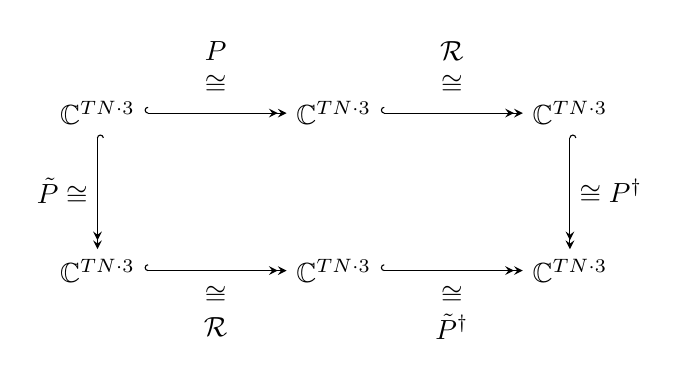
\begin{tikzpicture}[>=stealth, thin]
        \node (00) at (0, 0) {\(\mathbb{C}^{TN \cdot 3}\)};
        \node (01) at (3, 0) {\(\mathbb{C}^{TN \cdot 3}\)};
        \node (02) at (6, 0) {\(\mathbb{C}^{TN \cdot 3}\)};
        \node (10) at (0, -2) {\(\mathbb{C}^{TN \cdot 3}\)};
        \node (11) at (3, -2) {\(\mathbb{C}^{TN \cdot 3}\)};
        \node (12) at (6, -2) {\(\mathbb{C}^{TN \cdot 3}\)};
        \draw[{Hooks[right]}->>] (00) -- (01) node[above, pos=0.5] {\(\begin{array}{c}P\\\cong\end{array}\)};
        \draw[{Hooks[right]}->>] (01) -- (02) node[above, pos=0.5] {\(\begin{array}{c}\mathcal{R}\\\cong\end{array}\)};
        \draw[{Hooks[right]}->>] (02) -- (12) node[right, pos=0.5] {\(\cong P^\dagger\)};
        \draw[{Hooks[right]}->>] (00) -- (10) node[left, pos=0.5] {\(\tilde{P} \cong\)};
        \draw[{Hooks[right]}->>] (10) -- (11) node[below, pos=0.5] {\(\begin{array}{c}\cong\\\mathcal{R}\end{array}\)};
        \draw[{Hooks[right]}->>] (11) -- (12) node[below, pos=0.5] {\(\begin{array}{c}\cong\\\tilde{P}^\dagger\end{array}\)};
    \end{tikzpicture}
\end{minipage}

\begin{proof} We prove the statements in the order given.
    \begin{enumerate}[label=(\roman*), wide]
        \item \label{evol_time_theorem_1} The goal is to bound the term \(\norm*{U\ket{b}-\displaystyle\tilde{U}\ket{b}}\) for an arbitrary, but fixed \(\ket{b} \in \mathbb{C}^N\), as that suffices for a bound on \(\norm*{U-\tilde{U}}\), see \Cref{operator_norm}. Writing out \(\ket{\varphi}\) and \(\ket*{\tilde{\varphi}}\), we have
        \begin{align}
            \ket{\varphi} = U\ket{b} = \sum_{j=1}^N \beta_j \ket{0}\ket{v_j}\ket{h(\lambda_j)} \qquad \ket*{\tilde{\varphi}} = \tilde{U}\ket{b} = \tilde{P}^\dagger \sum_{j=1}^N \beta_j \sum_{k=0}^{T-1} \ajk \ket{k}\ket{v_j}\ket*{h(\tlk)}
        \end{align}
        Due to \Cref{state_similarity_theorem}, it suffices to bound \(\Re(\braket{\varphi}{\tilde{\varphi}})\) from below. Notice, that \(\tilde{P}\) is unitary, thus isometric due to \Cref{theorem_unitary_isometry}. This gives us:
        \begin{align}
            \braket*{\varphi}{\tilde{\varphi}} = \braket*{\tilde{P}\varphi}{\tilde{P}\tilde{\varphi}} &= \braket{\sum_{j=1}^N \beta_j\sum_{k=0}^{T-1} \ajk \ket{k}\ket{v_j}\ket{h(\lambda_j)}}{\sum_{j=1}^N \beta_j\sum_{k=0}^{T-1} \ajk \ket{k}\ket{v_j}\ket*{h(\tlk)}}\\
            &= \sum_{j=1}^N \sum_{k=0}^{T-1} |\beta_j\ajk|^2 \braket*{\ket{k}\ket{v_j}\ket{h(\lambda_j)}}{\ket{k}\ket{v_j}\ket*{h(\tlk)}}\\
            &\overset{\ref{evol_time_calc_1}}{=} \sum_{j=1}^N \sum_{k=0}^{T-1} |\beta_j\ajk|^2 \braket*{h(\lambda_j)}{h(\tlk)}
        \end{align}
        \begin{enumerate}[label=(\arabic*)]
            \item \label{evol_time_calc_1} We use \Cref{inner_tensor_prod_lemma}. 
        \end{enumerate}
        
        From that, we have
        \begin{align}
            \Re(\braket{\varphi}{\tilde{\varphi}}) = \sum_{j=1}^N \sum_{k=0}^{T-1} |\beta_j\ajk|^2 \Re(\braket*{h(\lambda_j)}{h(\tlk)})
        \end{align}
        Using \Cref{h_lipschitz} and \Cref{state_similarity_theorem}, we can observe:
        \begin{align}
            \norm*{\ket{h(\lambda_j)} - \ket*{h(\tlk)}} &= \sqrt{2(1-\Re(\braket*{h(\lambda_j)}{h(\tlk)}))} \leq \frac{\pi}{2}\kappa|\lambda_j-\tlk| \overset{\ref{evol_time_calc_2}}{=} \frac{\pi}{2}\kappa\left|\frac{\djk}{t_0}\right|\\
            &\leadsto \Re(\braket*{h(\lambda_j)}{h(\tlk)}) \geq 1 - \frac{\pi^2\kappa^2\djk^2}{8t_0^2}
        \end{align}
        \begin{enumerate}[label=(\arabic*)]
            \item \label{evol_time_calc_2} Since \(\tlk = \frac{2 \pi k}{t_0}\) by definition and thus \(t_0(\lambda_j-\tlk) = \lambda_jt_0 - 2\pi k = \djk\).
        \end{enumerate}
        
        We have
        \begin{align}
            &\phantom{=}\norm*{U\ket{b}-\tilde{U}\ket{b}}^2 = 2(1-\Re(\braket{\varphi}{\tilde{\varphi}})) \leq 2 \left(1-\left(\sum_{j=1}^N\sum_{k=0}^{T-1} |\beta_j\ajk|^2 \left(1-\frac{\pi^2\kappa^2\djk^2}{8t_0^2}\right)\right)\right)\\
            &= 2 \sum_{j=1}^N|\beta_j|^2\sum_{k=0}^{T-1} |\ajk|^2 \frac{\pi^2\kappa^2\djk^2}{8t_0^2} = 2\sum_{j=1}^N|\beta_j|^2\left(\sum_{\substack{k \in \mathbb{N}_{\leq T-1}\\|\djk| < 2\pi}} |\ajk|^2 \djk^2+\sum_{\substack{k \in \mathbb{N}_{\leq T-1}\\|\djk| \geq 2\pi}} |\ajk|^2 \djk^2\right)\frac{\pi^2}{8}\frac{\kappa^2}{t_0^2}\\
            &\overset{\ref{hhl_evol_time_calc_1}}{<} 2\sum_{j=1}^N|\beta_j|^2\left(8\pi^2 + \sum_{\substack{k \in \mathbb{N}_{\leq T-1}\\|\djk| \geq 2\pi}} \frac{22^2}{\djk^2}\right)\frac{\pi^2}{8}\frac{\kappa^2}{t_0^2} \overset{\ref{hhl_evol_time_calc_2}}{<} 2\sum_{j=1}^N|\beta_j|^2\left(8\pi^2 + 22^2 \cdot 2\sum_{k=1}^\infty \frac{1}{4\pi^2k^2}\right)\frac{\pi^2}{8}\frac{\kappa^2}{t_0^2}\\
            &\overset{\ref{hhl_evol_time_calc_3}}{=} 2\left(8 \pi^2 + \frac{2 \cdot 11^2 \cdot \pi^2}{90}\right)\frac{\pi^2}{8}\frac{\kappa^2}{t_0^2} < 261\frac{\kappa^2}{t_0^2}
        \end{align}
        \begin{enumerate}[label=(\arabic*)]
            \item \label{hhl_evol_time_calc_1} We upper-bound using \(|\djk| < 2 \pi\) directly on the left summation. We further use \Cref{basic_alpha_bound_and_alphas_are_prob_distr}, where the summation is over at most two values. On the right sum, we use \Cref{alpha_delta_values_relation} directly.

            \item \label{hhl_evol_time_calc_2} In the right term, use the fact, that the \(\djk\) values differ by an integer multiple of \(2\pi\) each to upper bound the summation term by the series \(\sum_{k=1}^\infty \frac{1}{4\pi^2k^2}\). After obtaining the bound, which is only dependent on \(\kappa^2/t_0^2\), we use \(\sum_{j=1}^N |\beta_j|^2 = 1\).
            
            \item \label{hhl_evol_time_calc_3} We use \Cref{zeta_two}. A consequence of this calculation is \(\sum_{j=1}^N |\beta_j|^2 \sum_{k=0}^{T-1} |\ajk|^2 \djk^2 < 106\).
        \end{enumerate}

        Since \(\ket{b}\) was chosen arbitrarily and \(\sqrt{261} < 17\), this concludes the proof.

        \item \label{evol_time_theorem_2} We use the notation from \Cref{special_lipschitz}. With the operator \(\tilde{P}\) from above, we have:
        \begin{align}
            \ket{x'} &= \frac{\sum_{j=1}^N \beta_j \ket{0}\ket{v_j}(f_j\ket{1}+g_j\ket{2})}{\sqrt{p'}} \text{ with } p' \coloneqq \sum_{j=1}^N |\beta_j|^2 (f_j^2+g_j^2)\\
            \ket{\tilde{x}'} &= \frac{\tilde{P}^\dagger \sum_{j=1}^N \beta_j \sum_{k=0}^{T-1} \ajk \ket{k}\ket{v_j}(\tilde{f}_k\ket{1}+\tilde{g}_k\ket{2})}{\sqrt{\tilde{p}'}} \text{ with } \tilde{p}' \coloneqq \sum_{j=1}^N \sum_{k=0}^{T-1} |\beta_j \ajk|^2 (\tilde{f}_k^2+\tilde{g}_k^2)
        \end{align}
        
        Notice \(p', \tilde{p}' \neq 0\). The maps \(j \mapsto f_j^2 + g_j^2\) and \((j, k) \mapsto \tilde{f}_k^2 + \tilde{g}_k^2\) may be interpreted as random variables in this context, where the associated probabilities are given by \(|\beta_j|^2\), and \(|\beta_j\ajk|^2\) respectively. We thus have \(p' = \expectation[f_j^2+g_j^2]\) and \(\tilde{p}' = \expectation[\tilde{f}_k^2 + \tilde{g}_k^2]\), where we omit the usual introduction of a formal random variable.

        We now proceed with the notation from \Cref{special_lipschitz}. With \Cref{inner_tensor_prod_lemma}, it holds, that
        \begin{align}
            \braket*{x'}{\tilde{x}'} = \braket*{\tilde{P} x'}{\tilde{P} \tilde{x}'} = \frac{\sum_{j = 1}^N |\beta_j|^2 \sum_{k=0}^{T-1} |\ajk|^2 \braket*{f_j\ket{1}+g_j\ket{2}}{\tilde{f}_k \ket{1}+\tilde{g}_k\ket{2}}}{\sqrt{p'\tilde{p}'}} = \frac{\expectation[f_j\tilde{f}_k+g_j\tilde{g}_k]}{\sqrt{p'\tilde{p}'}}
        \end{align}
        Furthermore, with the linearity of the expectation value \cite[p. 21]{Aigner2006}, we have
        \begin{align}
            \frac{\expectation[f_j\tilde{f}_k+g_j\tilde{g}_k]}{\sqrt{p'\tilde{p}'}} &= \frac{\expectation[f_j^2+g_j^2]+\expectation[(\tilde{f}_k-f_j)f_j+(\tilde{g}_k-g_j)g_j]}{\sqrt{p'\tilde{p}'}}\\
            &= \frac{1 + \expectation[(\tilde{f}_k-f_j)f_j+(\tilde{g}_k-g_j)g_j]/p'}{\sqrt{1+\frac{\tilde{p}'-p'}{p'}}}\\
            &\overset{\ref{hhl_expectation_error_calc_1}}{\geq} \left(1 + \frac{\expectation[(\tilde{f}_k-f_j)f_j+(\tilde{g}_k-g_j)g_j]}{p'}\right)\left(1-\frac{1}{2}\frac{\tilde{p}'-p'}{p'}\right)\\
            &\overset{\ref{hhl_expectation_error_calc_2}}{=} 1 - \frac{\expectation[(\tilde{f}_k-f_j)^2+(\tilde{g}_k-g_j)^2]}{2p'} - \frac{\expectation[(\tilde{f}_k-f_j)f_j+(\tilde{g}_k-g_j)g_j]}{p'}\frac{\tilde{p}'-p'}{2p'}
        \end{align}
        \begin{enumerate}[label=(\arabic*)]
            \item \label{hhl_expectation_error_calc_1} By using \Cref{inverse_sqrt_taylor_inequality} on \(\frac{1}{\sqrt{1+\frac{\tilde{p}'-p'}{p'}}}\).
            \item \label{hhl_expectation_error_calc_2} Using the linearity of expectation and \(\tilde{f}_k^2-f_j^2 = (\tilde{f}_k-f_j)(\tilde{f}_k+f_j) = (\tilde{f}_k-f_j)(\tilde{f}_k-f_j+2f_j)\), with the same statement for \(\tilde{g}_k\) and \(g_j\), we can expand
            \begin{align}
                \tilde{p}'-p' &= \expectation[\tilde{f}_k^2-f_j^2] - E[\tilde{g}_k^2-g_j^2]\\
                &= 2\expectation[(\tilde{f}_k-f_j)f_j]+2\expectation[(\tilde{g}_k-g_j)g_j]+\expectation[(\tilde{f}_k-f_j)^2]+\expectation[(\tilde{g}_k-g_j)^2]
            \end{align}
            With this formula, we have
            \begin{align}
                \expectation[(\tilde{f}_k-f_j)f_j+(\tilde{g}_k-g_j)g_j] = \frac{\tilde{p}'-p'}{2} - \frac{\expectation[(\tilde{f}_k-f_j)^2+(\tilde{g}_k-g_j)^2]}{2}
            \end{align}
            which we insert after expanding the parentheses.
        \end{enumerate}

        We first have
        \begin{align}
            \expectation[(\tilde{f}_k-f_j)^2+(\tilde{g}_k-g_j)^2] \overset{\ref{evol_time_calc_helper_1_1}}{\leq} \pi^2 \frac{\kappa^2}{t_0^2} \expectation[\djk^2(f_j^2+g_j^2)] \overset{\ref{evol_time_calc_helper_1_2}}{<} 106 \pi^2 \frac{\kappa^2}{t_0^2} p'
        \end{align}
        \begin{enumerate}[label=(\arabic*)]
            \item \label{evol_time_calc_helper_1_1} Using \Cref{special_lipschitz} in the expanded sum for the expectation value.
            \item \label{evol_time_calc_helper_1_2} In the proof of \ref{evol_time_theorem_1}, we have shown \(\expectation[\djk^2] < 106\). Especially,
            \begin{align}
                \sum_{k=0}^{T-1} |\ajk|^2\djk^2 < 106
            \end{align}
            for a fixed value of \(j\). So we observe
            \begin{align}
                \expectation[\djk^2(f_j^2+g_j^2)] = \sum_{j=1}^N |\beta_j|^2 (f_j^2+g_j^2) \sum_{k=0}^{T-1} |\ajk|^2\djk^2 < 106p'
            \end{align}
        \end{enumerate}
        Then
        \begin{align}
            \expectation[(\tilde{f}_k-f_j)f_j+(\tilde{g}_k-g_j)g_j] &\overset{\ref{evol_time_calc_helper_2_1}}{\leq} \expectation\left[\sqrt{(\tilde{f}_k-f_j)^2+(\tilde{g}_k-g_j)^2}\sqrt{f_j^2+g_j^2}\right]\\
            &\overset{\ref{evol_time_calc_helper_2_2}}{\leq} \pi\frac{\kappa}{t_0} \expectation\left[|\djk|(f_j^2+g_j^2)\right] \overset{\ref{evol_time_calc_helper_2_3}}{<} 11 \pi \frac{\kappa}{t_0} p'
        \end{align}
        \begin{enumerate}[label=(\arabic*)]
            \item \label{evol_time_calc_helper_2_1} Using \Cref{cauchy_schwarz_inequality}.
            \item \label{evol_time_calc_helper_2_2} Using \Cref{special_lipschitz}.
            \item \label{evol_time_calc_helper_2_3} Use \Cref{cauchy_schwarz_inequality} again, as well as \(E[\djk^2(f_j^2+g_j^2)] < 106p'\), for
            \begin{align}
                \expectation[|\djk|(f_j^2+g_j^2)] \leq \sqrt{E[\djk^2(f_j^2+g_j^2)]E[f_j^2+g_j^2]} < 11p'
            \end{align}
        \end{enumerate}

        Now for the last term involved, consider from the previous calculations
        \begin{align}
            \tilde{p}'-p' &= 2\expectation[(\tilde{f}_k-f_j)f_j+(\tilde{g}_k-g_j)g_j] + \expectation[(\tilde{f}_k-f_j)^2+(\tilde{g}_k-g_j)^2]\\
            &< 22\pi\frac{\kappa}{t_0}p'+106\pi^2\frac{\kappa^2}{t_0^2}p' \leq (22\pi+106\pi^2)\frac{\kappa}{t_0}p'
        \end{align}
        where we for now assume \(t_0 \geq \kappa\). Our choice of \(t_0\) later on will meet this condition.

        We now have
        \begin{align}
            \braket*{x'}{\tilde{x}'} > 1 - 53 \pi^2 \frac{\kappa^2}{t_0^2} - 11 \pi (11\pi + 53\pi^2) \frac{\kappa^2}{t_0^2} = 1 - \left(53 \pi^2  + 11 \pi (11\pi + 53\pi^2)\right) \frac{\kappa^2}{t_0^2} > 1-20000\frac{\kappa^2}{t_0^2}
        \end{align}
        yielding
        \begin{align}
            \norm*{\ket{x'}-\ket{\tilde{x}'}} < \sqrt{40000\frac{\kappa^2}{t_0^2}} = 200\frac{\kappa}{t_0}
        \end{align}

        \item \label{evol_time_theorem_3} Denote by \(p, \tilde{p}\) the success probability of either measurement, i.e. the probabilities of measuring a \(1\) for the qutrit when measuring \(\ket{\varphi}\) and \(\ket*{\tilde{\varphi}}\) respectively. We have \(p \neq 0\) and especially \(\tilde{p} \neq 0\) due to \Cref{existence_of_eigenvalue_approximations}. Measuring after whether the qutrit becomes \(1\) is equivalent to measuring first wrt. to the observable differentiating between whether the qutrit assumes the state \(\ket{0}\) or a state in \(\Span(\{\ket{1}, \ket{2}\})\) and then measuring for whether the qutrit becomes \(\ket{1}\). Consider first, that \(\ket{x} = \ket{x'}\), as well as \(p = p'\) due to \(g_j = 0\) for all \(j \in [1, N]_{\mathbb{N}}\). Then, we further have
        \begin{align}
            P\ket*{\tilde{x}} = \sqrt{\frac{\tilde{p}'}{\tilde{p}}}P\ket*{\tilde{x}'}-\sqrt{\frac{1}{\tilde{p}}}\sum_{j=1}^N \beta_j \sum_{k=0}^{T-1} \ajk \tilde{g}_k \ket{k}\ket{v_j}\ket{2}
        \end{align}
        from which we have
        \begin{align}
            \braket*{x}{\tilde{x}} = \braket{P\ket{x'}}{\sqrt{\frac{\tilde{p}'}{\tilde{p}}}P\ket*{\tilde{x}'}-\sqrt{\frac{1}{\tilde{p}}}\sum_{j=1}^N \beta_j \sum_{k=0}^{T-1} \ajk \tilde{g}_k \ket{k}\ket{v_j}\ket{2}} = \sqrt{\frac{\tilde{p}'}{\tilde{p}}}\braket*{P\ket{x'}}{P\ket*{\tilde{x}'}} > 1-20000\frac{\kappa^2}{t_0^2}
        \end{align}
        from which we obtain the statement directly using \ref{evol_time_theorem_2} and \(\tilde{p} \leq \tilde{p}'\).
    \end{enumerate}
\end{proof}

\begin{corollary}[Choosing \(t_0\)]
    To obtain an error smaller than \(\varepsilon\), we set
    \[
        t_0 \coloneqq 200 \frac{\kappa}{\varepsilon}
    \]
    Especially, as \(\varepsilon \in (0, 200)\), we have \(t_0 > \kappa\).
\end{corollary}

\paragraph*{Complexity Analysis} \phantom{}\\\phantom{}

We analyze each step in the algorithm, starting with the initialization procedures. First, the initialization of \(\ket{b}\). Denote the runtime term of \(\mathcal{B}\) as \(T_{\mathcal{B}}\). We make no assumptions on \(T_{\mathcal{B}}\), but for a fast runtime, it should be e.g. polynomial. For the clock register initialization, we have chosen \(t_0 \coloneqq 200 \frac{\kappa}{\varepsilon}\), so the condition
\begin{align}
    t_0 < 2 \pi T
\end{align}
for the bounds of the \(\djk\) values as in \Cref{inner_amplitude_bounds} gives \(t \coloneqq \lceil \log_2(\frac{100}{\pi}\frac{\kappa}{\varepsilon}) + 1 \rceil \in \onot(\log_2(\kappa/\varepsilon))\), or \(5\), which is asymptotically in the same class. The initialization of the clock register thus requires a complexity of \(\onot(t) = \onot(\log_2(\kappa/\varepsilon))\) following \Cref{quantum_state_generation_based_on_efficiently_integrable_probability_distributions}. The \(\qft\) can be efficiently implemented and its runtime shall be omitted here. The conditional Hamiltonian simulation adds the runtime
\begin{align}
    \tilde{\onot}\left(\log_2(N) \kappa s^4/\varepsilon\right)
\end{align}
following \Cref{hamiltonian_simulation}. We may note, that \(\norm{H} = 1\) by assumption, as we can directly calculate via the definition of the operator norm, see \Cref{operator_norm}, that the bound on the maximal eigenvalue also bounds the operator norm this way. We omit the runtime for the qutrit rotation for generating the auxiliary qutrit in the same manner as the \(\qft\). The last factor involved is AA, as in \Cref{amplitude_amplification}. For that, we consider first the following theorem on the success probability.
\begin{theorem}
    We have
    \begin{align}
        0 < \tilde{p} = \sum_{j=1}^N\sum_{k=0}^{T-1} |\beta_j\ajk|^2 \tilde{f}_k^2 \in \Omega(1/\kappa^2)
    \end{align}
\end{theorem}

\begin{proof}
    As proven in \Cref{existence_of_eigenvalue_approximations}, for each \(j\), there is are approximations \(k_j \in [0, T-1]_{\mathbb{N}}\) with \(|\lambda_j - \tilde{\lambda}_{k_j}| < \frac{1}{4\kappa}\). So \(\tilde{p} \neq 0\). Due to \(\tilde{\lambda}_{k_j} \in \left(\frac{3}{4\kappa}, 1 + \frac{1}{4\kappa}\right)\) and the strict monotonicity of \(f\) in both \(\left(\frac{3}{4\kappa}, 1\right]\) and \(\left[1, 1+\frac{1}{4\kappa}\right)\), we thus have
    \begin{align}
        \tilde{f}_{k_j}^2 &> \min\left(\left\{\frac{1}{4}\sin^2\left(\frac{\pi}{2}\left(2\frac{3}{4\kappa}-1\right)\right), \frac{1}{4\kappa^2\left(1+\frac{1}{4\kappa}\right)^2}\right\}\right) = \min\left(\left\{\frac{1}{4}\cos^2\left(\frac{3\pi}{4\kappa}\right), \frac{1}{4\kappa^2\left(1+\frac{1}{4\kappa}\right)^2}\right\}\right)\\
        &\geq \min\left(\left\{\frac{1}{8}, \frac{1}{(25/4)\kappa^2}\right\}\right) \in \Omega(1/\kappa^2)
    \end{align}
    To bound the associated \(|\ajk|^2\) values, we consider \Cref{alphas_yield_good_approximation}, which states
    \begin{align}
        \sum_{\substack{k \in [0, T-1]_{\mathbb{N}}\\|\djk| < 2\pi}} |\ajk|^2 > 0.3
    \end{align}
    This gives
    \begin{align}
        \tilde{p} > \sum_{j=1}^N |\beta_j|^2 \sum_{\substack{k \in [0, T-1]_{\mathbb{N}}\\|\djk| < 2\pi}} |\ajk|^2 \tilde{f}_k^2 \in \Omega\left(\frac{1}{\kappa^2}\right)
    \end{align}
    which is the statement.
\end{proof}

So the resulting runtime is
\begin{align}
    \tilde{\onot}(\kappa (T_{\mathcal{B}}+2\log_2(\kappa/\varepsilon)+\log_2(N)\kappa s^4/\varepsilon))
\end{align}

Let us summarize the result in one theorem.

\begin{theorem}[HHL Algorithm]
    Let \(N \coloneqq 2^n\), \(n \in \mathbb{N}_{\geq 1}\). Given a well-conditioned matrix \(A \in \mathbb{C}^{N \times N}\), an efficiently initializable state \(\ket{b} \in \mathbb{C}^N\) with initialization complexity term \(T_{\mathcal{B}}\), \(\ket{x} \coloneqq \frac{1}{\norm{A^{-1}\ket{b}}} A^{-1}\ket{b}\) and an error cap of \(\varepsilon \in (0, 100/(4\pi))\), there is a quantum algorithm for obtaining a quantum state \(\ket*{\tilde{x}} \in \mathbb{C}^N\) with \(\norm{\ket{\tilde{x}}-\ket{x}} < \varepsilon\) in time
    \begin{align}
        \tilde{\onot}(\kappa(T_{\mathcal{B}}+2\log_2(\kappa/\varepsilon)+\log_2(N)\kappa s^4 / \varepsilon))
    \end{align}
\end{theorem}

\subsection{Relaxations to the Assumptions and Discussion \draftcommentgreen{DONE}} \label{hhl_discussion}

\paragraph*{Relaxations} We deduce possible relaxations to the multitude of assumptions presented in \Cref{hhl_problem_description_and_assumptions}. Let \(A \in \mathbb{C}^{m \times n}\) be an arbitrary matrix and \(b \in \mathbb{C}^m\) be a vector, where \(m, n \in \mathbb{N}_{\geq 1}\). Consider the SLE \(Ax=b\), where \(x \in \mathbb{C}^n\) is unknown.

\begin{enumerate}[label=\arabic*.]
    \item If \(b = 0\), then \(x = 0\) is a solution. If \(A = 0\), then if \(b \neq 0\), there is no solution. Furthermore, if \(\norm{b} \neq 1\), then solving after \(Ax = \frac{b}{\norm{b}}\) gives the solution by \(\norm{b}x\). So we may now assume \(\norm{b} = 1\), \(A \neq 0\) and write \(\ket{b}\).
    \item If \(m \neq n\) and \(m\) is not a power of two, appending zero columns and rows to \(A\) and adding zero entries to \(\ket{b}\) gives a sufficient form of the equation system. In the next point, we describe a reduction, which suffices for introducing Hermiticity to create a system of form \((m+n) \times (m+n)\), so the number of rows and columns for \(A\) and zero entries for \(\ket{b}\) we need to add is given by \(1 \leq 2^{\lceil\log_2(m+n)\rceil}-(m+n) \leq 2^{\lceil \log_2(m+n)\rceil-1}-1\), which is polynomial. This modification further violates the invertibility requirement.
    \item \(\ket{b}\) must be efficiently initializable. There is no clear reduction strategy for this, except possibly preconditioning \cite[p. 4]{Harrow2008}, which we will also mention in connection with the sparsity.
    \item We first consider the Hermiticity requirement, before the invertibility. Hermiticity is needed to approximate the eigenvalues using an element of \(\frac{2 \pi \mathbb{Z}}{t_0}\) each. We may skip the following reduction, if the imaginary parts of the eigenvalues are very small, and the system is already quadratic. The latter point is needed for the second previous reduction, but can also be performed by appending additional rows or columns to the matrix and entries to the vector. In general, we can obtain a Hermitian matrix from \(A\) by performing the following reduction from \cite[p. 11-12]{Harrow2008} to a system of form
    \begin{align}
        \begin{pmatrix}
            0 & A\\
            A^\dagger & 0
        \end{pmatrix} \begin{pmatrix}
            0\\
            x
        \end{pmatrix} = \begin{pmatrix}
            \ket{b}\\
            0
        \end{pmatrix}
    \end{align}
    We verify the Hermiticity by
    \begin{align}
        \begin{pmatrix}
            0 & A\\
            A^\dagger & 0
        \end{pmatrix}^\dagger = \begin{pmatrix}
            0 & A^*\\
            A^t & 0
        \end{pmatrix}^t = \begin{pmatrix}
            0 & A\\
            A^\dagger & 0
        \end{pmatrix}
    \end{align}
    The space complexity of this reduction is given by the \(3mn\) additional entries to create the new matrix, but also by the \(n\) zero entries, which are added to \(\ket{b}\).

    \phantom{}

    We can further make statements about the eigenvalues and eigenstates of this matrix with the singular numbers and singular vectors of \(A\). Denote the matrix appearing in the reduction SLE as \(H \coloneqq \ket{0}\bra{1} \otimes A + \ket{1}\bra{0} \otimes A^\dagger\) and let the outer form of the SVD of \(A\) as in \Cref{theorem_svd} be given by
    \begin{align}
        A = \sum_{j=1}^r \sigma_j \ket{u_j}\bra{v_j} \text{ and thus } A^\dagger = \sum_{j=1}^r \sigma_j \ket{v_j}\bra{u_j}
    \end{align}
    with \(r \coloneqq \rk(A) > 0\), as \(A \neq 0\). We claim, that \(H\) has the \(2r\) eigenvalues \(\{\pm \sigma_j \mid j \in [1, r]_{\mathbb{N}}\}\) and \(2r\) eigenvectors \(\{\ket{w_j^{\pm}} \coloneqq (1/\sqrt{2})(\ket{0}\ket{u_j}\pm\ket{1}\ket{v_j}) \mid j \in [1, r]_{\mathbb{N}}\}\), which we can verify by direct matrix multiplication. Consider \(\ket{0}\ket{b}\), as in the reduction SLE, and express it via its projection
    \begin{align}
        \sum_{j=1}^r \braket{\ket{0}\ket{b}}{\ket{0}\ket{u_j}} \ket{0}\ket{u_j} = \sum_{j=1}^r \braket{b}{u_j} \ket{0}\ket{u_j} \eqqcolon \sum_{j=1}^r \beta_j \ket{0}\ket{u_j} = \sum_{j=1}^r \beta_j \frac{1}{\sqrt{2}}(\ket{w_j^+}+\ket{w_j^-})
    \end{align}
    using \Cref{inner_tensor_prod_lemma} and normalize it. Considerations regarding the fact, that we apply the algorithm on a projection of \(\ket{0}\ket{b}\), are made in the next point. Running the HHL algorithm gives an approximation of the state
    \begin{align}
        \sum_{j=1}^r \frac{\beta_j}{\sigma_j} \frac{1}{\sqrt{2}}(\ket{w_j^+}-\ket{w_j^-})
    \end{align}
    under normalization.
    \item \label{invertibility_reductions} If \(A\) is not invertible, then first need to reconsider the initial problem statement. If we have \(\ket{b} \notin \Im(A)\), there is no target state to approximate, but if \((\lambda_1, \ket{v_1}), ..., (\lambda_N, \ket{v_N})\) again denotes the eigenvalue-eigenstate pairs of an eigenbasis of \(A\), then can define \(P_{\Im} \coloneqq \sum_{\lambda_j \neq 0} \ket{v_j}\bra{v_j}\) and \(P_{\ker} \coloneqq \sum_{\lambda_j = 0} \ket{v_j}\bra{v_j}\) to be the image and kernel projectors of \(A\). The HHL algorithm then seemingly approximates the solution to the SLE problem
    \begin{align}
        A\ket{x} = \frac{1}{\norm{P_{\Im}\ket{b}}} P_{\Im}\ket{b}
    \end{align}
    if \(P_{\Im}\ket{b} \neq 0\). But this is also not the case in general. Defining \(P_w \coloneqq \sum_{\lambda_j \in \left[\frac{1}{\kappa}, 1\right]} \ket{v_j}\bra{v_j}\) and \(P_b \coloneqq \sum_{\lambda_j \notin \left[\frac{1}{\kappa}, 1\right]} \ket{v_j}\bra{v_j}\) to be the projectors into the \emph{well-conditioned subspace} and \emph{bad-conditioned subspace}
    \begin{align}
        \Span\left(\left\{\ket{v_j} \; \middle| \; j \in [1, N]_{\mathbb{N}}, \lambda_j \in \left[\frac{1}{\kappa}, 1\right]\right\}\right) \text{ and } \Span\left(\left\{\ket{v_j} \; \middle| \; j \in [1, N]_{\mathbb{N}}, \lambda_j \notin \left[\frac{1}{\kappa}, 1\right]\right\}\right)
    \end{align}
    and especially besides the contributions of the projection of \(\ket{b}\) onto the subspace
    \begin{align}
        \Span\left(\left\{\ket{v_j} \; \middle| \; j \in [1, N]_{\mathbb{N}}, \lambda_j \in \left(\frac{1}{2\kappa}, \frac{1}{\kappa}\right) \cup \left(1, \infty\right)\right\}\right)
    \end{align}
    due to the actions of the filter functions in \((1/(2\kappa), 1/\kappa)\) and afterwards, the HHL algorithm solves the SLE
    \begin{align}
        A\ket{x} = \frac{1}{\norm{P_{w}\ket{b}}} P_{w}\ket{b}
    \end{align}
    if \(P_{w}\ket{b} \neq 0\). The filter functions still perform ''true'' inversion in the space spanned by the eigenstates associated with eigenvalues in \((1, \infty)\), but when these values become very large, their contributions also vanish.

    \phantom{}
    
    Besides that, there is no division by zero inside of the algorithm, if there are eigenvalues of value zero, but the solution to the SLE may be wrong to an unacceptable degree due to the filter functions possibly filtering out most of the contribution by \(P_b\ket{b}\). One further issue, which follows from this problem, is, that if \(\braket{b}{v_j} = 0\) for all \(j \in [1, N]_{\mathbb{N}}\) with \(\lambda_j \in \left(\frac{1}{2\kappa}, \infty\right)\), the algorithm does not terminate in general, as the amplitude amplification does not terminate, see \Cref{amplitude_amplification}. The success probability of measuring a \(1\) must be greater than zero, as required in our analysis of the complexity.
    
    \phantom{}

    In summary, there is no clear general strategy for generally solving this issue, and for the application of the algorithm to succeed these projections must be taken into consideration, although we also discuss strategies for scaling the eigenvalues for enlargening the well-conditioned subspace. As Harrow et al. may have implied it \cite[p. 7]{Harrow2008}, a person working with the algorithm may in general want to weigh the contribution of the well-conditioned and bad-conditioned subspaces first.
    \item The requirement for positive-semidefiniteness mainly affects the phase estimation analysis in \Cref{hhl_phase_estimation_analysis}, but also the analysis of the filter functions for the overall error. As we aim to approximate \(\lambda_j t_0\) for any fixed \(j \in [1, N]_{\mathbb{N}}\) and \(t_0 > 0\), the algorithm must allow \(k < 0\). We can do that by increasing the clock register size by \(1\), so \(t \gets t + 1\) in the following, and additionally applying the conditioned phase transformation
    \begin{align}
        N\colon \mathbb{C}^{T} \to \mathbb{C}^{T}, \ket{\tau} \mapsto e^{i\frac{\tau}{T} \cdot 2\pi\left(\frac{T}{2}-1\right)}\ket{\tau}
    \end{align}
    on the clock register before the application of \(\qft^\dagger\) in \Cref{hhl_algorithm}. This map is unitary and efficiently implementable, as considering the binary representation \(\tau = \tau_{t-1}...\tau_0 = \sum_{i=0}^{t-1} \tau_i 2^i\) of an index \(\tau \in [0, T-1]_{\mathbb{N}}\) gives
    \begin{align}
        N = \bigotimes_{i=0}^{t-1} \begin{pmatrix}
            e^{\frac{0}{T}\cdot 2\pi \left(\frac{T}{2}-1\right)} & 0\\
            0 & e^{\frac{2^{(t-1)-i}}{T}\cdot 2\pi \left(\frac{T}{2}-1\right)}
        \end{pmatrix}
    \end{align}
    The state after the phase estimation using this phase transformation is thus
    \begin{align}
        \frac{\sqrt{2}}{T} \sum_{j = 1}^N \beta_j \sum_{k = 0}^{T-1} \left(\sum_{\tau = 0}^{T-1} \sin\left(\frac{\pi(\tau+\frac{1}{2})}{T}\right) e^{\frac{i \tau}{T} \left(\lambda_j t_0 - 2 \pi \left(k-\left(\frac{T}{2}-1\right)\right)\right)}\right) \ket{k} \ket{v_j} \ket{0}
    \end{align}
    This gives
    \begin{align}
        k - \left(\frac{T}{2}-1\right) \in \left[-\left(\frac{T}{2}-1\right), \frac{T}{2}\right]
    \end{align}
    Modifying the algorithm in this way does not change any of the results from the phase estimation analysis, but it allows the existence of a \(k\) with \(|\djk| < 2\pi\) for any \(j\). These approximations should then be denoted by \(\tlk \coloneqq \frac{2\pi}{t_0} (k - (T/2-1))\). We uncompute the registers analogously. We further need to mirror the filter functions at \(y = 0\) to allow for negative approximations, similarly to Childs et al. \cite[p. 5]{Childs2015}. The statements of the Lipschitz-continuity of \(\ket{h(\cdot)}\) in \Cref{the_hhl_algorithm} and the proof of the special Lipschitz-type condition in \Cref{special_lipschitz} do not change either, because for the first we only considered the derivatives and for the second, we mirrored the filter functions. And, since \Cref{evol_time_theorem} and the complexity analysis are also not affected, this reduction solves the problem.
    \item Here we have no clear reduction of the sparsity of \(A\). Possible techniques may include performing basis switches or simply considering simulation techniques for different Hamiltonians\footnote{In this sense, we can consider the Hamiltonian simulation as replaceable.} following \cite[p. 6]{Harrow2008} or even allowing the use of a \emph{preconditioner} \cite[p. 4]{Harrow2008}, which would make the problem more suitable for the HHL algorithm.
    \item Efficient row-computability is essential to the Hamiltonian simulation time. We refer to the last point.
    \item For \(\frac{1}{\kappa} \leq \lambda_j \leq 1\) for all \(j \in [1, N]_{\mathbb{N}}\), we first consider in the positive-semidefinite case, that the contribution of the space spanned by the eigenstates with eigenvalue \(\lambda_j > 1\) vanishes with larger \(\lambda_j\) in the inversion by the filter function \(f\). If we still need this requirement, for instance since many eigenvalue contributions come from eigenvalues in \((0, 1/(2\kappa)]\), then we may consider calculating the maximal condition number \(\lambda_{\max} \in \mathbb{R}_{> 0}\) and then by \(A\frac{1}{\lambda_{\max}}x = \ket{b}\), we have indeed this requirement for the eigenvalues in this SLE. This is due to our ability to scale the Hamiltonian, which in return scales the eigenvalues due to \((\mu A)\ket{v_j} = (\mu\lambda_j)\ket{v_j}\) for any \(\mu \in \mathbb{R}\), \(j \in [1, N]_{\mathbb{N}}\). We recover the solution vector for the original system by multiplying with \(\lambda_{\max}\). When using an upper bound, we must consider, if our approximation or upper bound for \(\kappa\) does not cut off eigenvalues, which become very small by dividing by \(\lambda_{\max}\). For \(\lambda_{\min} = 1\) or \(\lambda_{\min} \approx 1\), it would also suffice to use \(\kappa\) as this maximum eigenvalue bound. If we have only negative eigenvalues, we can multiply \(A\) with \(-1\) and in case of having both positive and negative eigenvalues, we cannot additively shift the eigenvalues, so the only clear reduction strategy would be to weigh both subspaces and multiply by \(-1\), iff the subspace spanned by the eigenstates of the negative eigenvalues has a larger contribution for the accuracy of the solution.
    \item We may omit the requirement for having the exact value of \(\kappa\) by providing an upper bound on it, similarly to Childs et al. \cite[p. 3]{Childs2015}. This affects mainly the filter functions and the algorithm runtime. How such an upper bound can be obtained is generally unclear, but we have seen one instance, where one can do that, when we discussed the example of the condition number of \emph{Hilbert matrices}, see \Cref{example_hilbert_matrices}. Another strategy involves increasing \(\kappa\) exponentially by \(1, 2, 4, ...\), as \cite[p. 6]{Harrow2008} suggest. For that, we would still need to have a success probability of the measurement, which is not equal to zero, as otherwise AA does not terminate.
\end{enumerate}

\paragraph*{Discussion and Outlook} Our description of the original HHL algorithm is finished. We want to now discuss some chosen aspects.

\phantom{}

We first want to give some remarks regarding the original HHL paper and why we needed some more technical lemmas in this thesis. First, the initialization of the clock state is not further elaborated, only a small mention of it is made in \cite[p. 2]{Harrow2008}. As a sidenote, we may consider it to be interesting, that we can obtain the formula for the antiderivative using the formula by Brassard et al.. The calculation of the alternative representation of the \(\ajk\) values in \Cref{alpha_values_rewrite} contains mistakes, due to which the result is off by \(-1/2\). The phase estimation analysis presented \cite[pp. 10-11]{Harrow2008} concludes with a bound of \(|\ajk| \leq \frac{8\pi}{\djk^2}\), using the lower bound in \Cref{sine_bound}, but it is not applicable, as, see our argument immediately after \Cref{inner_amplitude_bounds}, the assumption \(|\djk| \leq T/10\) is generally wrong and thus the arguments of the sine functions can be in \([3.5\pi/4, \pi]\), which supersedes the root \(\sqrt{6}\) of the lower bounding polynomial \(x-x^3/6\), which leads to both terms of the product \(\sin\left(\frac{\djk + \pi}{2T}\right)\sin\left(\frac{\djk - \pi}{2T}\right)\) in the denominator becoming negative. Furthermore, in \cite[p. 6]{Harrow2008}, a description of the actual implementation of qutrit rotation is missing.

\phantom{}

The choice of initial coefficients for the clock register is seemingly arbitrary. Harrow et al. reason, that it suites the error analysis well \cite[p. 2]{Harrow2008}, which it does, but the optimality has not been shown. From our research, it appears, that this aspect of the algorithm has not been further studied. Some authors instead suggest in their diagrams, that we can initialize the register by applying the Hadamard transformation. Examples of this constitute \cite[p. 30]{Dervovic2018}, \cite[p. 351]{Kasirajan2021} and \cite[p. 5]{Lee2019}. It would seem, that most experimental setups prefer this initialization procedure, although it does not conform to the original description and especially does not fulfill the requirements for the guaranteed bounds from the error analysis.

\phantom{}

Some experimental implementations of the algorithm further fix the evolution time to \(2\pi\), see \cite[p. 4-5]{Cao2011} for a demonstration. This parameter can, in most cases, be chosen in a better way, as we argue in the next example. In the example of Cao et al., they also do not initialize using the clock register using the proposed coefficients, and they do not use the filter functions. Although in this case, this could be due to the example being of pure demonstrational nature. In general, the choices of \(t\) and \(t_0\) do not need to be fixed, especially, if we possibly consider a nyche case.
\begin{example}
    Suppose all eigenvalues are in \(\mathbb{N}_{\geq 1}\). Then we can choose \(t\) at least large enough, s.t. \(T-1 \geq \max\{\lambda_1, ..., \lambda_N\}\) and \(t_0 \coloneqq 1\). In this case, the eigenvalue estimation is near perfect for all eigenvalues. Suppose \(\lambda_j = k\), then \(\djk = 0\) and, by \Cref{alpha_values_rewrite}, we have
    \begin{align}
        |\ajk| &= \frac{\sqrt{2}}{T} \frac{1}{\sin(\frac{\pi}{2T})} > \frac{\sqrt{2}}{T} \frac{2T}{\pi} = \frac{2\sqrt{2}}{\pi} > 0.9003
    \end{align}
    under the use of \Cref{sine_bound}.
\end{example}

\phantom{}

To improve numerical stability, specific filter functions were chosen. The authors state, that the choice of \(f\) and \(g\) is arbitrary \cite[p. 6]{Harrow2008}. This aspect could be studied further to find out, if the numerical precision can be improved by choosing different functions. We also argue, that a straight cut-off at the boundary \(\frac{1}{\kappa}\) would suffice for most needs. A dive into the referred literature at \cite[p. 6]{Harrow2008} may also help improve the general understanding regarding this point.

\phantom{}

We want to again consider the initial problem statement for the HHL algorithm. The goal was to solve an SLE. After we have seen the actual operations of the HHL algorithm, it is valid to ask what exact answer the HHL algorithm is approximating. In our discussion of possible relaxation techniques for the invertibility of \(A\), see \ref{invertibility_reductions}, we observed, that the result of the algorithm is an inversion of the projection of the given vector into the so-called well-conditioned subspace of eigenstates of \(A\). The result of the algorithm is thus not always the actual solution to the SLE itself. We know, that in general, there may be no solutions, exactly one or several more, neither case can always be determined using the HHL algorithm. In some cases, as in Chen and Gaos algorithm for obtaining solutions of polynomial equation systems, which we present in \Cref{chen_and_gaos_results}, one can decide the solvability by studying a special case and more techniques.

\phantom{}

Furthermore, the result of the HHL algorithm is a quantum state, not a classical vector. The no-cloning-theorem \cite[pp. 81-84]{Homeister2018}, in practice, thus makes the duplication of the result state impossible. Obtaining the entries of a quantum state is in general not a trivial task, although there have been suggestions for such methods \cite[pp. 14-25]{Brassard2000}. HHL can thus only be used as a subroutine in a larger quantum or hybrid quantum algorithm, which makes its applicability in some fields, such as machine learning or cryptography, difficult.

\phantom{}

We believe, that the given runtime for the Hamiltonian simulation in \cite[p. 6]{Harrow2008} is off by a factor of \(\onot(s^2)\). We have detailled our calculation for the runtime of the method used in \Cref{hamiltonian_simulation}, while in the original HHL paper, there is no mention of where to find or derive the claimed runtime. The researchers Childs et al., who are actively involved in the research of Hamiltonian simulation, as for instance \cite{Childs2010,Childs2015} show, have further supported this claim in \cite[p. 2]{Childs2010}. If this finding is true, then the runtime of the HHL algorithm is as analyzed approximately \(\tilde{\onot}(\log_2(N)\kappa^2s^4/\varepsilon)\) and not \(\tilde{\onot}(\log_2(N)\kappa^2s^2/\varepsilon)\), which could have far reaching consequences regarding the research applying the HHL algorithm, of which we mention some recent results in the next paragraph.

\phantom{}

In the next subsection, we will discuss two improvements of the algorithm by Ambainis and Childs et al.. To add to this, we have in general found, that since the release of the paper, the algorithm has been extended and applied by multiple authors, as Harrow et al. themselves have observed \cite[pp. 4-5]{Harrow2008}. For instance by using it to solve \emph{non-linear differential equations} \cite{Leyton2008}, as such problems can often be reduced to linear systems \cite{Forster2017}. \cite{BravoPrieto2019} presents four more improvements in its introduction and the \emph{Variational Quantum Linear Solver} (VQLS), an algorithm, that combines a minimization problem for a cost function on a classical computer with a quantum algorithm for solving SLEs. Hybrid quantum-classical algorithms have been developed and tested, one such test constitutes \cite{Lee2019}, thus giving a different class of quantum SLE solvers than HHL-inspired ones.

\subsection{Outline of Two Improvements \draftcommentgreen{DONE}}

We want to briefly mention two improved algorithms based on the ideas of HHL.

\paragraph*{Variable Time Amplitude Amplification} \phantom{}\\\phantom{}

Ambainis suggested a model of gate quantum computation, in which a quantum algorithm could ''halt'' at different times, and derived another algorithm for solving linear systems of equations based on HHL \cite{Ambainis2010}. We will explain the model briefly and then summarize the result.

\paragraph*{Branched Quantum Computations} The model of VTAA \cite[pp. 5-8]{Ambainis2010} is based on a state space of form \(\mathcal{H} \coloneqq \mathbb{C}^3 \otimes \mathcal{H}_o\), where \(\mathcal{H}_o\) is a Hilbert space. The system, or our register, shall be in the states \(\ket{\psi_1}, ..., \ket{\psi_m} \in \mathcal{H}\) at times \(t_1, ..., t_m \in \mathbb{R}_{\geq 0}\). Every \(t_i\), \(i \in [1, m]_{\mathbb{N}}\), the system may \emph{stop}, meaning that we stop the algorithm with a given probability \(p_i \in [0, 1]\). We require
\begin{enumerate}
    \item that there are subspaces \(\mathcal{H}_i\) of \(\mathcal{H}_o\) forming an ascending chain \(\mathcal{H}_1 \subseteq \mathcal{H}_2 \subseteq ... \subseteq \mathcal{H}_m = \mathcal{H}_o\).
    \item \label{vtaa_second_requirement} that we can express \(\ket{\psi_i}\) for an \(i \in [1, m]_{\mathbb{N}}\) as
    \begin{align}
        \ket{\psi_i} = \alpha_{i, 0} \ket{0} \otimes \ket{\psi_{i, 0}} + \alpha_{i, 1} \ket{1} \otimes \ket{\psi_{i, 1}} + \alpha_{i, 2} \ket{2} \otimes \ket{\psi_{i, 2}}
    \end{align}
    where \(\alpha_{i, 0}, \alpha_{i, 1}, \alpha_{i, 2} \in \mathbb{C}\) are scalars and \(\ket{\psi_{i, 0}}, \ket{\psi_{i, 1}} \in \mathcal{H}_i\), as well as \(\ket{\psi_{i, 2}} \in \mathcal{H}_o \cap \mathcal{H}_i^\perp\) may not necessarily be valid quantum states. We further have \(\ket{\psi_{m, 2}} = 0\).
    \item Let \(i \in [1, m-1]_{\mathbb{N}}\) be fixed. Denote by \(P_{\mathcal{H}_i}\) the projector into \(\mathcal{H}_i\). Then
    \begin{align}
        \ket{\psi-{i, 0}} = P_{\mathcal{H}_i}\ket{\psi_{i+1, 0}} \land \ket{\psi-{i, 1}} = P_{\mathcal{H}_i}\ket{\psi_{i+1, 1}}
    \end{align}
\end{enumerate}
We may interpret this model the following way: During computation, parts of our state switch the Hilbert space, in which the main calculation is currently performed. By doing that, we are enabling the possibility of dovetailing, i.e. interweaving multiple computations. The interpretation of the states comes from requirement \ref{vtaa_second_requirement}: Similar to the HHL algorithm, \(\ket{\psi_{i, 1}}\) decodes the ''good'' part of the state and \(\ket{\psi_{i, 0}}, \ket{\psi_{i, 2}}\) decode the bad parts of the state. The desired results of the computation itself are thus contained inside of \(\mathcal{H}_i\) at time \(t_i\) respectively.

\begin{figure}[!hbtp]
    \centering
    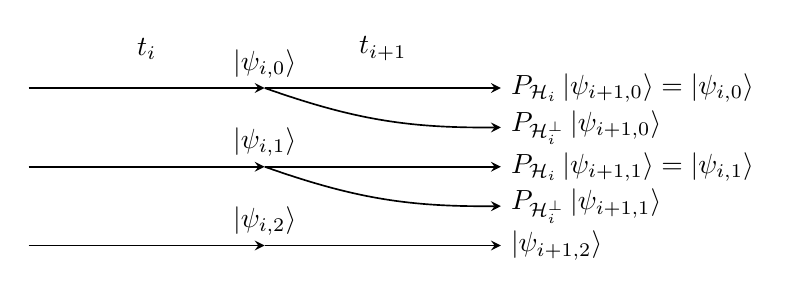
\begin{tikzpicture}[>=stealth, semithick]
        \node at (1.5, 0) {\(t_i\)};
        \draw[->] (0, -0.5) -- (3, -0.5) node[above] {\(\ket{\psi_{i, 0}}\)};
        \draw[->] (3, -0.5) -- (6, -0.5) node[right] {\(P_{\mathcal{H}_i}\ket{\psi_{i+1, 0}} = \ket{\psi_{i, 0}}\)};
        \draw (3, -0.5) edge[->, bend right=10] node[pos=1.0, right] {\(P_{\mathcal{H}_{i}^\perp} \ket{\psi_{i+1, 0}}\)} (6, -1.0);
        \draw[->] (0, -1.5) -- (3, -1.5) node[above] {\(\ket{\psi_{i, 1}}\)};
        \draw[->] (3, -1.5) -- (6, -1.5) node[right] {\(P_{\mathcal{H}_i}\ket{\psi_{i+1, 1}} = \ket{\psi_{i, 1}}\)};
        \draw (3, -1.5) edge[->, bend right=10] node[pos=1.0, right] {\(P_{\mathcal{H}_{i}^\perp} \ket{\psi_{i+1, 1}}\)} (6, -2.0);
        \draw[->] (0, -2.5) -- (3, -2.5) node[above] {\(\ket{\psi_{i, 2}}\)};
        \draw[->] (3, -2.5) -- (6, -2.5) node[right] {\(\ket{\psi_{i+1, 2}}\)};
        \node at (4.5, 0) {\(t_{i+1}\)};
    \end{tikzpicture}
    \caption{Illustation of the difference between the three components of two different consecutive states in a VTAA algorithm, where \(i \in [1, m]_{\mathbb{N}}\) is fixed. The branches in the arrows indicate sums, i.e. e.g. \(\ket{\psi_{i, 0}} = P_{\mathcal{H}_i}\ket{\psi_{i, 0}} + P_{\mathcal{H}_i^\perp}\ket{\psi_{i, 0}}.\)}
    \label{vtaa_illustration}
\end{figure}

The times \(t_1, ..., t_m\) and probabilities \(p_1, ..., p_m\) were let lose by us and are up to the algorithm designer to choose. As Ambainis, one may define the \emph{average stopping time} by
\begin{align}
    T_a \coloneqq \sqrt{\sum_{i=1}^m p_i t_i^2}
\end{align}
and set the maximum time \(T_M \coloneqq t_m\) and the success probability at time point \(t_m\) to be \(p_s \coloneqq |\alpha_{m, 1}|^2\). Ambainis then proves the following theorem.

\begin{theorem}
    There is a quantum algorithm, which amplifies the success probability of an algorithm in the VTAA model to give a successful measurement in time
    \begin{align}
        \onot\left(T_M\log^{0.5}(T_M)+\frac{T_a}{p_s}\log^{1.5}(T_M)\right)
    \end{align}
\end{theorem}

The main result by Ambainis is now, that by expressing the HHL algorithm inside of the VTAA model, we can improve the success probability from \(\onot(\kappa^2)\) wrt. the runtime factor of \(\kappa\). There we had \(\onot(\kappa^2)\) as the dependence, which was obtained by choosing the evolution time in dependence of \(\onot(\kappa)\) and then running AA for another dependence on \(\onot(\kappa)\). Ambainis acquires the following result \cite[pp. 8-12]{Ambainis2010}.

\begin{theorem}
    Using VTAA, there is a quantum algorithm, which improves the runtime of the HHL algorithm to
    \begin{align}
        \tilde{\onot}\left(\log_2(N) \kappa \log_2^3\left(\frac{\kappa}{\varepsilon}\right) s^2 \log_2^2\left(\frac{1}{\varepsilon}\right) \frac{1}{\varepsilon^3}\right)
    \end{align}
\end{theorem}

The runtime cited comes from the fact, that the phase estimation procedure of runtime \(\onot(\log_2(N) \kappa s^2 / \varepsilon)\) is used as a subprocedure of the algorithm \cite[p. 9]{Ambainis2010}, but Ambainis omits the \(\onot(\log_2(N) s^2)\) factor in \cite[p. 12]{Ambainis2010}. Note, that we cited the runtime factor \(\onot(s^2)\) to conform with these papers, although it should be \(\onot(s^4)\).

\begin{remark}
    We may note, that while the dependence on \(\kappa\) is better than the original HHL algorithm, the error dependence is significantly worse.
\end{remark}

\paragraph*{Fourier Decompositions for Sublinear Error Dependence} \label{hhl_fourier_approach} \phantom{}\\\phantom{}

In a 2015 paper, Childs et al. presented three approaches \cite{Childs2015} to substantially improving the error dependence of the HHL algorithm. We shortly describe the so-called \emph{Fourier approach}, which we shall divide into the explanation of three conceptual steps.

\begin{itemize}
    \item First, the results include the use of newer techniques for the Hamiltonian simulation, as presented by Childs et al. in \cite{Berry2015}.
    \item Secondly, one important aspect of the paper is the use of LCUs as in \cite[pp. 5-8]{Childs2015}. Let \(A \in \mathbb{C}^{N \times N}, N \coloneqq 2^n, n \in \mathbb{N}_{\geq 1}\) be the matrix of the SLE. Assume further it is, possibly after a reduction, Hermitian and assume for the sake of the conceptual overview, that it is invertible. The idea is then to, similiarly to the Hamiltonian decomposition in \Cref{hamiltonian_simulation}, decompose the matrix \(A^{-1}\) into a unitary sum and to simulate the sum. The unitaries chosen are indeed \(e^{iAt_j}\), where \(t_j \in \mathbb{R}\) are times, giving a decomposition of form \(A^{-1} = \sum_{j}\alpha_je^{iAt_j}\) with coefficients \(\alpha_j \in \mathbb{C}\). By performing a basis switch, the authors then reduce the problem of approximating this decomposition to approximating a real univariate decomposition \(x^{-1} = \sum_j \alpha_j e^{ixt_j}\) for \(x \in [-1, -1/\kappa] \cup [1/\kappa, 1]\).
    \item Thirdly, to compute the aforementioned decomposition of \(1/x\), the following Fourier transformation is used:
    \begin{align}
        \frac{1}{x} = \frac{i}{\sqrt{2\pi}}\int_0^\infty\int_{-\infty}^\infty ze^{-z^2/2}e^{-ixyz} \; dz \; dy
    \end{align}
    As in \cite[pp. 10-11]{Childs2015}. It is shown how to discretize these integrals, giving a suitable quantum algorithm for approximating \(A^{-1}\).
\end{itemize}
We recognize again the pattern of using an efficient decomposition of the initial linear operator for solving the SLE problem. Childs et al. then have as one of their results the following theorem as in \cite[p. 4]{Childs2015}.
\begin{theorem}[Fourier Approach to HHL]
    Using more recent results for Hamiltonian simulation, techniques involving LCUs and Fourier transformations, there is a quantum algorithm for solving an SLE in time
    \begin{align}
        \onot\left(s\kappa^2\log_2^{2.5}\left(\frac{\kappa}{\varepsilon}\right)\left(\log_2(N)+\log_2^{2.5}\left(\frac{\kappa}{\varepsilon}\right)\right)\right)
    \end{align}
\end{theorem}

The other two approaches include the use of \emph{Chebyshev polynomials} and the modification of Ambainis' VTAA HHL algorithm. The three approaches are not equivalent, as pointed out in \cite[p. 4]{Childs2015} and have their own advantages and disadvantages, which we shall not elaborate, as this is a high level overview of the results.

    \section{Application on the Cryptanalysis of AES} \label{application_on_the_cryptanalysis_of_aes}

The AES, synonymously \emph{Rijndael}, is a famous, widely used block cipher. It is specified by the US-American NIST in \cite{Dworkin2001}. AES is a symmetric cipher, meaning that it uses one key for the encryption and decryption of blocks. The key is \(K\) bits long, where \(K \in \{128, 192, 256\}\). Thus, it is clear that for a brute force approach to key retrieval with Grovers algorithm, one can achieve a quadratic improvement from a runtime of \(\onot(2^K)\) to \(\onot(2^{K/2})\).

Rijndael and AES are two different cipher specifications. As described by the original authors of both ciphers \cite[p. 31]{Daemen_2020}, the difference lies in the allowed values of the input block length and the cipher key length. We will focus on AES, as it is the cipher of our cryptanalytical interest.

The goal of this last subsection is twofold. For one, we want to discuss the inner workings of Rijndael and its formulation as a so-called BES-cipher. Especially, we want to form a system of equations for key recovery using that, which we will however not solve, as this is not the scope of this thesis. Secondly, we will discuss current research on this topic in the context of two recent papers by the researchers Chen and Gao \cite{Chen2017} and Ding et al. \cite{Ding2021}. We chose BES, as it overcomes a small algebraic problem when attempting to formulate such an equation system with a comparatively simple solution. We furthermore analyze the size of the system.

AES has proven to be a reliable cipher over the years, resisting any attempt at successful cryptanalysis yet, as a survey by Nover shows \cite{Nover}. The authors of Rijndael, Joan Daemen and Vincent Rijmen, released a book on the details and the design philosophy of Rijndael \cite{Daemen_2020}, as referenced above. It shall be our main source for the next subsection, next to the FIPS cipher specification.

\subsection{An Algebraic Description of AES \draftcommentgreen{DONE}} \label{an_algebraic_description_of_aes}

An overview of AES is given in \Cref{aes_block_diagram}. \Cref{aes_parameters} lists the relevant parameters. We shall use the symbol \(K\) for the key itself. One difficulty in this description is differentiating between the different representations of bytes: A byte can be seen as a vector from the vector space \(\gf(2)^8\), an integer from the finite modulo ring \(\mathbb{F}_{2^8}\) or as a polynomial from the field \(\gf(2)[x]/(p)\), where \(p \in \gf(2)[x]\) is an irreducible polynomial, see \Cref{byte_field}. We shall explicitely state the form we use each time. We always index starting from the least significant bit, so for instance we may have \(b = b_7b_6b_5b_4b_3b_2b_1b_0 = 01110010\), which corresponds to \((0, 1, 0, 0, 1, 1, 1, 0)^t\), \(114\) or \(x^6+x^5+x^4+x\).

The input of the algorithm is both a \(32N_b\)-bit plaintext \(P \in \mathbb{F}_{2^8}^{4 \times N_b}\) and a \(32N_k\)-bit key \(K \in \mathbb{F}_{2^8}^{4 \times N_k}\). The output is a \(32N_b\)-bit long encrypted block \(C \in \mathbb{F}_{2^8}^{4 \times N_b}\). We will describe each step of the AES in detail and algebraically. We also do not fix \(N_b\), \(N_r\) or \(N_k\), as it is not necessary for our discussion.

One major design criterion of AES was space-efficiency \cite[pp. 4-5]{Daemen_2020}, thus, we do not require a lot of storage. We work with a null-indexed column-major enumeration of the input plaintext bytes along a \(4 \times N_b\) grid following \cite[p. 9]{Dworkin2001}. Let the plaintext be the initial \emph{state} \(S \coloneqq (s_{(i-1)(j-1)})_{i, j \in 4 \times N_b} \in \mathbb{F}_{2^8}^{4 \times N_b}\) of the current encryption or decryption. The plaintext indices start at the first byte, independent of endianness. In other words, \(S = P\) and, since \(P = (p_0, ..., p_{4N_b-1}) \in \mathbb{F}_{2^8}^{4N_b} \cong \mathbb{F}_{2^8}^{4 \times N_b}\), we can write for both \(P\) and \(K\) analogously
\begin{align}
    P = S = \begin{pmatrix}
        p_{ 0} & p_{ 4} & p_{ 8} & p_{12}\\
        p_{ 1} & p_{ 5} & p_{ 9} & p_{13}\\
        p_{ 2} & p_{ 6} & p_{10} & p_{14}\\
        p_{ 3} & p_{ 7} & p_{11} & p_{15}
    \end{pmatrix} \qquad K = \begin{pmatrix}
        k_{ 0} & k_{ 4} & k_{ 8} & k_{12}\\
        k_{ 1} & k_{ 5} & k_{ 9} & k_{13}\\
        k_{ 2} & k_{ 6} & k_{10} & k_{14}\\
        k_{ 3} & k_{ 7} & k_{11} & k_{15}
    \end{pmatrix}
\end{align}
for the initial state \cite[p. 33]{Daemen_2020}, here for the case \(N_b = N_k = 4\).

\begin{table}[!hbtp]
    \centering
    \begin{tabular}{|c|c|c|c|}
        \hline
        Parameter & Meaning & AES-128, AES-192, AES-256\\
        \hline
        \(N_b\) & Block length in 32-bit words. & 4, 4, 4\\
        \(K\) & Length of cipher key in bits. & 128, 192, 256\\
        \(N_k\) & Key length in 32-bit words. & 4, 6, 8\\
        \(N_r\) & Round count. & 10, 12, 14\\
        \hline
    \end{tabular}
    \caption{AES Parameters, according to \cite[pp. 13-14]{Dworkin2001}.}
    \label{aes_parameters}
\end{table}

\begin{figure}[!hbtp]
    \centering
    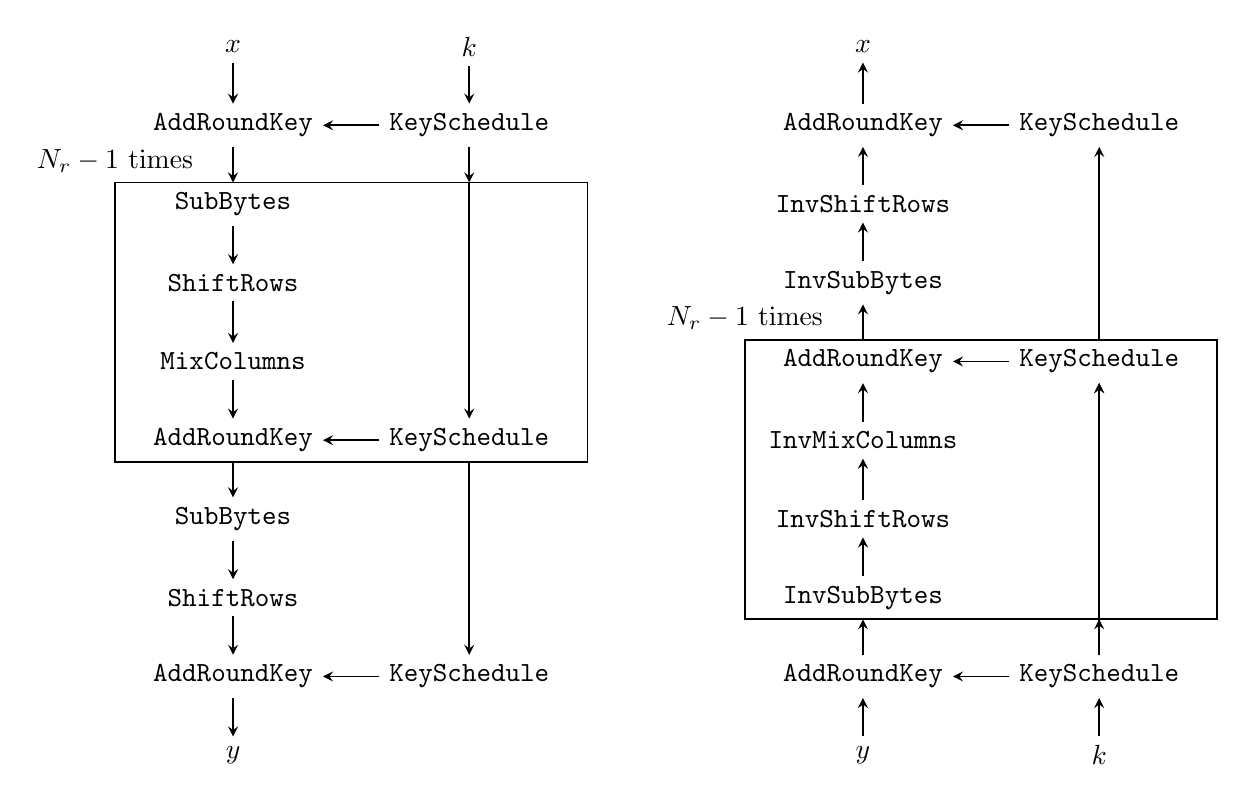
\begin{tikzpicture}[>=stealth, semithick]
        \node (x) at (0, 0) {\(x\)};
        \node[below of=x] (s11) {\texttt{AddRoundKey}};
        \node[below of=s11] (s21) {\texttt{SubBytes}};
        \node[below of=s21] (s22) {\texttt{ShiftRows}};
        \node[below of=s22] (s23) {\texttt{MixColumns}};
        \node[below of=s23] (s24) {\texttt{AddRoundKey}};
        \node[below of=s24] (s31) {\texttt{SubBytes}};
        \node[below of=s31] (s32) {\texttt{ShiftRows}};
        \node[below of=s32] (s33) {\texttt{AddRoundKey}};
        \node[below of=s33] (y) {\(y\)};
        \draw[->] (x) -- (s11);
        \draw[->] (s11) -- (s21);
        \draw[->] (s21) -- (s22);
        \draw[->] (s22) -- (s23);
        \draw[->] (s23) -- (s24);
        \draw[->] (s24) -- (s31);
        \draw[->] (s31) -- (s32);
        \draw[->] (s32) -- (s33);
        \draw[->] (s33) -- (y);
        \draw ($(s21.north)+(-1.5, 0)$) rectangle ($(s24.south)+(4.5, 0)$);
        %\draw ($(s31.north)+(-1.5, 0)$) rectangle ($(s33.south)+(4.5, 0)$);
        %\node[left] at ($(s22.south)+0.5*(s23.north)-0.5*(s22.south)-(1.5, 0)$) {\(N_r-1\) times};
        \node[above] at ($(s21.north)+(-1.5, 0)$) {\(N_r-1\) times};
        \node (k) at ($(x)+(3, 0)$) {\(k\)};
        \node (k1) at ($(s11)+(3, 0)$) {\texttt{KeySchedule}};
        \node (k2) at ($(s24)+(3, 0)$) {\texttt{KeySchedule}};
        \node (k3) at ($(s33)+(3, 0)$) {\texttt{KeySchedule}};
        \draw[->] (k) -- (k1);
        \draw[->] (k1) -- ($(s21.north)+(3, 0)$);
        \draw[->] ($(s21.north)+(3, 0)$) -- (k2);
        \draw[->] (k2) -- (k3);
        \draw[->] (k1) -- (s11);
        \draw[->] (k2) -- (s24);
        \draw[->] (k3) -- (s33);

        \node (x) at (8, 0) {\(x\)};
        \node[below of=x] (i33) {\texttt{AddRoundKey}};
        \node[below of=i33] (i32) {\texttt{InvShiftRows}};
        \node[below of=i32] (i31) {\texttt{InvSubBytes}};
        \node[below of=i31] (i24) {\texttt{AddRoundKey}};
        \node[below of=i24] (i23) {\texttt{InvMixColumns}};
        \node[below of=i23] (i22) {\texttt{InvShiftRows}};
        \node[below of=i22] (i21) {\texttt{InvSubBytes}};
        \node[below of=i21] (i11) {\texttt{AddRoundKey}};
        \node[below of=i11] (y) {\(y\)};
        \draw[<-] (x) -- (i33);
        \draw[<-] (i33) -- (i32);
        \draw[<-] (i32) -- (i31);
        \draw[<-] (i31) -- (i24);
        \draw[<-] (i24) -- (i23);
        \draw[<-] (i23) -- (i22);
        \draw[<-] (i22) -- (i21);
        \draw[<-] (i21) -- (i11);
        \draw[<-] (i11) -- (y);
        \draw ($(i24.north)+(-1.5, 0)$) rectangle ($(i21.south)+(4.5, 0)$);
        \node[above] at ($(i24.north)+(-1.5, 0)$) {\(N_r-1\) times};
        \node (k3) at ($(i33)+(3, 0)$) {\texttt{KeySchedule}};
        \node (k2) at ($(i24)+(3, 0)$) {\texttt{KeySchedule}};
        \node (k1) at ($(i11)+(3, 0)$) {\texttt{KeySchedule}};
        \node (k) at ($(y)+(3, 0)$) {\(k\)};
        \draw[->] (k) -- (k1);
        \draw[->] (k1) -- ($(i21.south)+(3, 0)$);
        \draw[->] ($(i21.south)+(3, 0)$) -- (k2);
        \draw[->] (k1) -- (k2);
        \draw[->] (k2) -- (k3);
        \draw[->] (k1) -- (i11);
        \draw[->] (k2) -- (i24);
        \draw[->] (k3) -- (i33);
    \end{tikzpicture}
    \caption{AES encryption and decryption block diagram. The inverse versions of the encryption functions are defined in analogy to them, and will not be of concern to us.}
    \label{aes_block_diagram}
\end{figure}

\begin{enumerate}[label=(\roman*)]
    \item \label{aes_subbytes} \texttt{SubBytes} \cite[pp. 34-37]{Daemen_2020}: Each byte in the state is interpeted as an element of the field \(F \coloneqq \gf(2)[x]/(x^8+x^4+x^3+x+1)\). First, consider the so-called \emph{patched inverse} bijection \(\iota\), as well as the matrix \(L_A \in \gf(2)^{8 \times 8}\) and vector \(v_A \in \gf(2)^8\):
    \begin{align}
        \iota\colon F \overset{\cong}{\to} F, a \mapsto \begin{cases}
            0 & a = 0\\
            a^{-1} & a \neq 0
        \end{cases} \qquad L_A \coloneqq \begin{pmatrix}
            1&0&0&0&1&1&1&1\\
            1&1&0&0&0&1&1&1\\
            1&1&1&0&0&0&1&1\\
            1&1&1&1&0&0&0&1\\
            1&1&1&1&1&0&0&0\\
            0&1&1&1&1&1&0&0\\
            0&0&1&1&1&1&1&0\\
            0&0&0&1&1&1&1&1
        \end{pmatrix} \qquad v_A \coloneqq \begin{pmatrix}
            1\\
            1\\
            0\\
            0\\
            0\\
            1\\
            1\\
            0
        \end{pmatrix}
    \end{align}
    The \texttt{SubBytes} step performs the map
    \begin{align}
        \rho\colon F \to F, a \mapsto L_A \iota(a) + v_A
    \end{align}
    for each byte \(s\) in \(S\). This part of the description already poses a problem for the cryptanalysis of the cipher, as we switched from \(F\) to \(\gf(2)^8\) for the application of the affine transformation. \(\rho\) is also called the \emph{Rijndael S-Box}. We may also note, that the byte is interpreted as a column vector with the top entry being the LSB. \(L_A\) is further invertible, as \(\det(L_A) = 5\), which we may check in a long calculation via the recursive development of the determinant.
    \item \texttt{ShiftRows} \cite[pp. 37-38]{Daemen_2020}: Use the following map:
    \begin{align}
        \begin{pmatrix}
            s_{00} & s_{01} & s_{02} & s_{03}\\
            s_{10} & s_{11} & s_{12} & s_{13}\\
            s_{20} & s_{21} & s_{22} & s_{23}\\
            s_{30} & s_{31} & s_{32} & s_{33}\\
        \end{pmatrix} \mapsto \begin{pmatrix}
            s_{00} & s_{01} & s_{02} & s_{03}\\
            s_{11} & s_{12} & s_{13} & s_{10}\\
            s_{22} & s_{23} & s_{20} & s_{21}\\
            s_{33} & s_{30} & s_{31} & s_{32}\\
        \end{pmatrix}
    \end{align}
    We can also express this operation via a permutation matrix \(M_A \in F^{4N_b \times 4N_b}\). The above instruction is then equivalent to taking a row-major enumeration of \(S\) and performing
    \begin{align}
        S \mapsto S_A S
    \end{align}
    where we denote with the notation of a permutation, i.e. each entry shows the index of the \(1\)-entry in the column
    \begin{align}
        S_A \coloneqq (0, 5, 10, 15, 4, 9, 14, 3, 8, 13, 2, 7, 12, 1, 6, 11)
    \end{align}
    \item \texttt{MixColumns} \cite[pp. 39-41]{Daemen_2020}: The \(i \in [0, N_b-1]_{\mathbb{N}}\)th column vector \((s_{ij})_{j \in [0, 3]_{\mathbb{N}}}\) of \(S\) is treated as a vector from \(F' \coloneqq \mathbb{F}_{2^8}[x]/(x^4+1)\) and multiplied with \(3x^3+x^2+x+2\). This is equivalent to taking a column-major enumeration of \(S\) and applying the diagonal matrix \(M_A \coloneqq \diag(C_A, C_A, C_A, C_A)\), where
    \begin{align}
        C_A \coloneqq \begin{pmatrix}
            2 & 3 & 1 & 1\\
            1 & 2 & 3 & 1\\
            1 & 1 & 2 & 3\\
            3 & 1 & 1 & 2
        \end{pmatrix}
    \end{align}
    following \Cref{polynomial_multipl_matrix_example}. Note, that the first byte in a column thus corresponds to the coefficient \(x^3\) in each polynomial, and so on.
    \item \texttt{AddRoundKey} \cite[p. 41]{Daemen_2020}: During the \(i \in [0, N_r]_{\mathbb{N}}\)th round, add the current round key, so \(S \mapsto S + \tilde{K}_i\). See \ref{key_schedule}.
    \item \label{key_schedule} \texttt{KeySchedule} \cite[pp. 43-46]{Daemen_2020}: The algorithm initially creates \(N_r+1\) additional keys \(\tilde{K}_0, ..., \tilde{K}_{N_r} \in \mathbb{F}_{2^8}^{4 \times N_b}\) for the \texttt{AddRoundKey} step. This procedure is called \texttt{KeyExpansion}. Let \(W \coloneqq \mathbb{F}_{2^8}^{4 \times N_b(N_r+1)}\) be a matrix of \(N_b(N_r+1)\) \(32\)-bit words. Four columns each correspond to a round key. We further define so-called \emph{round constants} \(r_{i+1} \coloneqq x^i \in F\), \(i \in \mathbb{N}\). All additions are performed in \(\gf(2)^8\), so by a component-wise exclusive-or operation.
    
    There are versions of the \texttt{KeyExpansion} for \(N_k \leq 6\) and \(N_k > 6\). For AES, these versions correspond to the cases \(N_k \in \{4, 6\}\) and \(N_k = 8\). If \(N_k \leq 6\), then the matrix \(W\) is constructed column by column according to the following rules, in this order of precedence:
    \begin{align}
        \begin{array}{rll}
            w_{ij} &\coloneqq k_{ij} & i \in [0, 3]_{\mathbb{N}}, j \in [0, N_k-1]_{\mathbb{N}}\\
            w_{0j} &\coloneqq w_{0(j-N_k)} + \rho(w_{1(j-1)}) + r_{j/N_k} & j \in [N_k, N_b(N_r+1)-1]_{\mathbb{N}}, j = 0 \bmod N_k\\
            w_{ij} &\coloneqq w_{i(j-N_k)} + \rho(w_{((i+1) \bmod 4)(j-1)}) & i \in [1, 3]_{\mathbb{N}}, j \in [N_k, N_b(N_r+1)-1]_{\mathbb{N}}, j = 0 \bmod N_k\\
            w_{ij} &\coloneqq w_{i(j-N_k)} + w_{i(j-1)} & i \in [0, 3]_{\mathbb{N}}, j \in [N_k, N_b(N_r+1)-1]_{\mathbb{N}}, j \neq 0 \bmod N_k
        \end{array}
    \end{align}
    If \(N_k > 6\), then the matrix \(W\) is constructed in a similar way, that is according to:
    \begin{align}
        \begin{array}{rll}
            w_{ij} &\coloneqq k_{ij} & i \in [0, 3]_{\mathbb{N}}, j \in [0, N_k-1]_{\mathbb{N}}\\
            w_{0j} &\coloneqq w_{0(j-N_k)} + \rho(w_{1(j-1)}) + r_{j/N_k} & j \in [N_k, N_b(N_r+1)-1]_{\mathbb{N}}, j = 0 \bmod N_k\\
            w_{ij} &\coloneqq w_{i(j-N_k)} + \rho(w_{((i+1) \bmod 4)(j-1)}) & i \in [1, 3]_{\mathbb{N}}, j \in [N_k, N_b(N_r+1)-1]_{\mathbb{N}}, j = 0 \bmod N_k\\
            w_{ij} &\coloneqq w_{i(j-N_k)} + \rho(w_{i(j-1)}) & i \in [0, 3]_{\mathbb{N}}, j \in [N_k, N_b(N_r+1)-1]_{\mathbb{N}}, j = 4 \bmod N_k\\
            w_{ij} &\coloneqq w_{i(j-N_k)} + w_{i(j-1)} & i \in [0, 3]_{\mathbb{N}}, j \in [N_k, N_b(N_r+1)-1]_{\mathbb{N}}, j \neq 0 \bmod N_k
        \end{array}
    \end{align}
    After \(W\) is obtained, we derive the keys by \(W = \begin{pmatrix}
        \tilde{K}_0 & \tilde{K}_1 & ... & \tilde{K}_{N_r}
    \end{pmatrix}\).
\end{enumerate}
The output of the algorithm is stored in \(S\). We may also note, that all steps described are invertible, allowing decryption.

\subsection{The BES Cipher \draftcommentgreen{DONE}} \label{the_bes_cipher}

The cryptanalysis of AES in form of the above algebraic description is complicated, as we have to switch between the field \(F\) and the vector space \(\gf(2)^8\). The \emph{Big Encryption System} (BES) cipher by Murphy and Robshaw \cite{Murphy2002} defines a family of ciphers similar structure, and simplifies the cryptanalysis by only using operations in \(F\). We shall describe the BES for every version of AES and without the so-called modified key schedule \cite[p. 3]{Murphy2002}.\footnote{As a sidenote, that the authors of AES proposed a similar method as described here under the name of \emph{AES-GF}, see \cite[pp. 192-194]{Daemen_2020}.}

\phantom{}

We define the map
\begin{align}
    \phi \colon F &\to F^8\\
    b &\mapsto \left(b^{\left(2^0\right)}, b^{\left(2^1\right)}, ..., b^{\left(2^7\right)}\right)
\end{align}
For any \(n \in \mathbb{N}_{\geq 1}\), \(\phi\) is extended component-wise, giving
\begin{align}
    \phi_n \colon F^n &\to F^{8n}\\
    b &\mapsto \left(\phi(b_1), \phi(b_2), ..., \phi(b_n)\right)
\end{align}
Analogously, we define the matrix operation \(\phi_{m \times n}\), \(m \in \mathbb{N}_{\geq 1}\), via \(\phi_{mn}\). We further let
\begin{align}
    \iota(\phi(a)) \coloneqq \phi(\iota(a))
\end{align}
with \(\iota\) being the patched inverse, as described in the AES \texttt{SubBytes} operation, see \ref{aes_subbytes} in the previous subsection. The component-wise application of \(\iota\) gives the analogous definitions for the general functions \(\phi_n\) and \(\phi_{m \times n}\).

\begin{theorem}[Properties of \(\phi\)]
    \(\phi\) is injective and additive. Both properties carry over to \(\phi_n\). \footnote{Field theorists may be reminded of the \emph{Frobenius homomorphism} \cite[p. 337]{Fischer2017}. The additivity there, the \emph{Frobenius rule}, is also called \emph{the freshmans dream}. The proof idea for the additivity is the same.}
\end{theorem}

\begin{proof}
    The injectivity can be read off by observing the behavior on the first component. For the additivity we calculate in \(\gf(2)[X]\) and \(k \in [0, 7]_{\mathbb{N}}\) using the binomial development:
    \begin{align}
        (a+b)^{\left(2^k\right)} = \sum_{l=0}^{2^k} \binom{2^k}{l} a^l b^{2^k-l} = a^{\left(2^k\right)} + b^{\left(2^k\right)}
    \end{align}
    Note that the terms for \(1 \leq l \leq 2^k-1\) vanish as the binomial factors are natural numbers and especially divisible by \(2\). We slightly abuse the notation here, but the point is, that the terms in the middle of the sum are evenly often added together, which leads to the polynomial powers vanishing.
\end{proof}

\phantom{}

As mentioned, the main result by Murphy and Robshaw is, that we can represent the AES algorithm by only using operations in \(F\). It is not yet clear, why \(\phi\) could help our cause. In the same manner as in \Cref{an_algebraic_description_of_aes}, we shall describe all five operations in the language of BES. For that, we first map the input plaintext-key pair \((P, K)\) via \(\phi\) into the BES-associated vector spaces. So now, denote \(P \in \left(F^8\right)^{4 \times N_b}\), \(K \in \left(F^8\right)^{4 \times N_k}\) and for the state \(S \in \left(F^8\right)^{4 \times N_b}\). Also \(C \in \left(F^8\right)^{4 \times N_b}\), as we will see.

\begin{enumerate}[label=(\roman*')]
    \item \texttt{SubBytes} \cite[pp. 5-8]{Murphy2002}: The patched inverse \(\iota\) can be applied component-wise for each entry \(s_{ij}\) in S. In the original AES, we applied the operator \(L_A\colon \gf(2)^8 \to \gf(2)^8\) after \(\iota\) and then added \(v_A\). This is an operation in \(\gf(2)^8\), not \(F\), and it is not clear, how we could represent this operation with a linear transformation. Define
    \begin{align}
        \psi\colon F \to \gf(2)^8, \sum_{k=0}^7 b_kx^k \mapsto \begin{pmatrix}
            b_0\\
            ...\\
            b_7
        \end{pmatrix}
    \end{align}
    to be the bijective natural embedding of \(F\) into \(\gf(2)^8\). Then, we form the map \(f \coloneqq \psi^{-1} \circ L_A \circ \psi\). For the following derivation, we want a polynomial, which interpolates \(f\). The Lagrangian interpolation method \cite[p. 193]{Fischer2017} gives
    \begin{align}
        f(x) = \sum_{b \in F} f(b) \prod_{c \in F \setminus \{b\}} \frac{x-c}{b-c} = \sum_{k=0}^7 \lambda_k x^{\left(2^k\right)}
    \end{align}
    with \((\lambda_i)_{i \in [0, 7]_{\mathbb{N}}} \coloneqq (\texttt{05}, \texttt{09}, \texttt{f9}, \texttt{25}, \texttt{f4}, \texttt{01}, \texttt{b5}, \texttt{8f})\) in hexadecimal notation following \cite[p. 7]{Murphy2002}, where we do not verify this result here, as this would require a large computation using a computer, for which we know the needed multiplication techniques. \(L_A\) is invertible and thus \(f\). Interpret the hexadecimal notation here digit-wise, so e.g. \(\texttt{f9} = 11111001\).

    Similarly to \(\phi\), \(f\) is additive. For the matrix representing the action of the linear map \(L_A\), we may choose
    \newcommand{\lampow}[2]{\lambda_{#1}^{\left(2^{#2}\right)}}
    \begin{align}
        \hat{L}_B \coloneqq \left(\lampow{j-1}{i-1}\right)_{i, j \in 8 \times 8} = \begin{pmatrix}
            \lampow{0}{0} & \lampow{1}{0} & \lampow{2}{0} & \lampow{3}{0} & \lampow{4}{0} & \lampow{5}{0} & \lampow{6}{0} & \lampow{7}{0}\\
            \lampow{7}{1} & \lampow{0}{1} & \lampow{1}{1} & \lampow{2}{1} & \lampow{3}{1} & \lampow{4}{1} & \lampow{5}{1} & \lampow{6}{1}\\
            \lampow{6}{2} & \lampow{7}{2} & \lampow{0}{2} & \lampow{1}{2} & \lampow{2}{2} & \lampow{3}{2} & \lampow{4}{2} & \lampow{5}{2}\\
            \lampow{5}{3} & \lampow{6}{3} & \lampow{7}{3} & \lampow{0}{3} & \lampow{1}{3} & \lampow{2}{3} & \lampow{3}{3} & \lampow{4}{3}\\
            \lampow{4}{4} & \lampow{5}{4} & \lampow{6}{4} & \lampow{7}{4} & \lampow{0}{4} & \lampow{1}{4} & \lampow{2}{4} & \lampow{3}{4}\\
            \lampow{3}{5} & \lampow{4}{5} & \lampow{5}{5} & \lampow{6}{5} & \lampow{7}{5} & \lampow{0}{5} & \lampow{1}{5} & \lampow{2}{5}\\
            \lampow{2}{6} & \lampow{3}{6} & \lampow{4}{6} & \lampow{5}{6} & \lampow{6}{6} & \lampow{7}{6} & \lampow{0}{6} & \lampow{1}{6}\\
            \lampow{1}{7} & \lampow{2}{7} & \lampow{3}{7} & \lampow{4}{7} & \lampow{5}{7} & \lampow{6}{7} & \lampow{7}{7} & \lampow{0}{7}
        \end{pmatrix}
    \end{align}
    The seemingly arbitrary choices for the bottom \(15\) rows root in the concept of \(\phi\) being a map mapping into \emph{field conjugates}, a concept relating to minimal polynomials \cite[p. 286]{Karpfinger_2017}, which we shall not dive into. Notice
    \begin{align}
        (\hat{L}_B \phi(b))_0 = \sum_{k=0}^7 \lambda_k b^{\left(2^k\right)} = f(b)
    \end{align}
    for any \(b \in F\), which was the desired action. As for \(v_A\), let \(v_B \coloneqq \phi(v_A)\) and add it to the state byte. To apply the matrix on the entire state, it suffices to form the diagonal matrix composed of \(4N_b\) \(L_B\) blocks and add \(v_B\) to each entry, while using \(S\) in a column-major enumeration.
    \item \texttt{ShiftRows} \cite[pp. 5-6]{Murphy2002}: The shifting of the \(F^8\) elements inside \(S\) is the same as in the original AES. The matrix \(M_A\) is generalized to \(M_B\) by replacing every one with \(E_8\) for a \(F^{16N_b \times 16N_b}\) permutation matrix performing this action.
    \item \texttt{MixColumns} \cite[p. 6]{Murphy2002}: In the AES, we could represent this step as a matrix multiplication with \(M_A\). In BES, we analogously define
    \begin{align}
        C_B^k \coloneqq \begin{pmatrix}
            2^{\left(2^k\right)} & 3^{\left(2^k\right)} & 1 & 1\\
            1 & 2^{\left(2^k\right)} & 3^{\left(2^k\right)} & 1\\
            1 & 1 & 2^{\left(2^k\right)} & 3^{\left(2^k\right)}\\
            3^{\left(2^k\right)} & 1 & 1 & 2^{\left(2^k\right)}
        \end{pmatrix} \in F^{4 \times 4}
    \end{align}
    for \(k \in [0, 7]_{\mathbb{N}}\). This matrix has the property
    \begin{align}
        C_B^k \left(y_0^{\left(2^k\right)}, y_1^{\left(2^k\right)}, y_2^{\left(2^k\right)}, y_3^{\left(2^k\right)}\right)^t = \left(z_0^{\left(2^k\right)}, z_1^{\left(2^k\right)}, z_2^{\left(2^k\right)}, z_3^{\left(2^k\right)}\right)^t
    \end{align}
    for \(y, z \in F^4\), preserving the aforementioned so-called conjugacy property. We may now set
    \begin{align}
        M_B \coloneqq \begin{pmatrix}
              C_B^0 & \cdots &      0 & \cdots &      0 &      0 &      0\\
             \vdots & \ddots & \vdots & \cdots &      0 &      0 &      0\\
                  0 & \cdots &  C_B^7 & \cdots &      0 &      0 &      0\\
             \vdots & \vdots & \vdots & \ddots & \vdots & \vdots & \vdots\\
                  0 &      0 &      0 & \cdots &  C_B^0 & \cdots &      0\\
                  0 &      0 &      0 & \cdots & \vdots & \ddots & \vdots\\
                  0 &      0 &      0 & \cdots &      0 & \cdots &  C_B^7
        \end{pmatrix} \in F^{32N_b \times 32N_b}
    \end{align}
    Multiplying with \(S\) in column-major enumeration, while enumerating its entries from \(F^8\) as row vectors gives the desired map.
    \item \texttt{AddRoundKey} \cite[p. 5]{Murphy2002}: We perform the same addition as in Rijndael \(S \mapsto S + \tilde{K}_i\) in the \(i \in [0, N_r]\)th round.
    \item \texttt{KeySchedule} \cite[p. 8]{Murphy2002}: All operations in the key schedule have been explained in the explanations of the previous suboperations, so we can carry it over identically by, instead of using \(F\) as the bytes in the key expansion array \(W \in (F^8)^{4 \times 4N_b(N_r+1)} \cong F^{32 \times 4N_b(N_r+1)}\), the operations being addition and the map \(\rho\), which takes on the form \(b \mapsto \hat{L}_B(\iota(b_0), ..., \iota(b_7))^t+v_B\), and the polynomial addition. The round constants are also thus \(\phi(r_j)\), \(j \in \mathbb{N}_{\geq 1}\).
\end{enumerate}

We may summarize this discussion with the following theorem.

\begin{theorem}
    If \(\alpha\colon F^{4 \times N_b} \times F^{4 \times N_k} \to F^{4 \times N_b}\) denotes the AES cipher and \(\beta\colon F^{32 \times N_b} \times F^{32 \times N_k} \to F^{32 \times N_b}\) its associated BES-cipher respectively, then the following diagram commutes:

    \begin{minipage}{\linewidth}
        \centering
        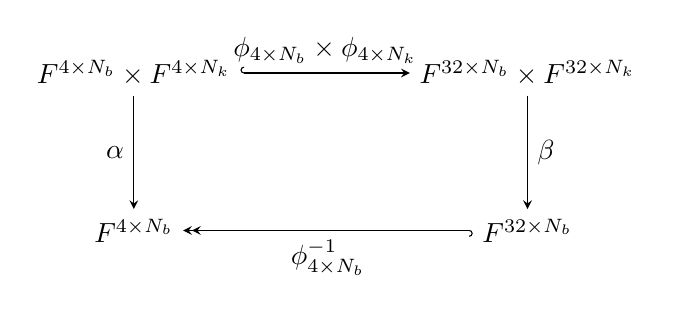
\begin{tikzpicture}[>=stealth, thin]
            \node (00) at (0, 0) {\(F^{4 \times N_b}  \times F^{4 \times N_k}\)};
            \node (01) at (5, 0) {\(F^{32 \times N_b} \times F^{32 \times N_k}\)};
            \node (10) at (0, -2) {\(F^{4 \times N_b}\)};
            \node (11) at (5, -2) {\(F^{32 \times N_b}\)};
            \draw[{Hooks[right]}->] (00) -- (01) node[above, pos=0.5] {\(\phi_{4 \times N_b} \times \phi_{4 \times N_k}\)};
            \draw[->] (01) -- (11) node[right, pos=0.5] {\(\beta\)};
            \draw[{Hooks[right]}->>] (11) -- (10) node[below, pos=0.5] {\(\phi_{4 \times N_b}^{-1}\)};
            \draw[->] (00) -- (10) node[left, pos=0.5] {\(\alpha\)};
        \end{tikzpicture}
    \end{minipage}
\end{theorem}
Note that in the above diagram, cartesian products of functions are functions taken component-wise and the arguments of \(\alpha\) and \(\beta\) are in order (plaintext, key).

\subsection{A BES Multivariate Equation System for AES \draftcommentgreen{DONE}}

With the previous description of BES for AES, we can now form a multivariate equation system for key recovery over \(F\). Note, that we do not follow Murphy and Robshaw with the derivation of their multivariate quadratic equation system in \cite[pp. 11-13]{Murphy2002}. Consider the description of AES in \Cref{aes_block_diagram}. We are given a plaintext \(P \in (F^8)^{4 \times N_b}\) and a ciphertext \(C \in (F^8)^{4 \times N_b}\), where we know, that \(C\) was produced from \(P\) via running BES using a key \(K \in (F^8)^{4 \times N_k}\). We have an initial addition of the first \(4 \times N_b\) sized part of the key \(K\), which is \(\tilde{K}_0\), giving the state \(S_0\), then execute \(N_r-1\) ''normal'' rounds of AES before entering the last round, where \texttt{MixColumn} is omitted.
\begin{align}
    P \mapsto S_0 \mapsto S_1 \mapsto ... \mapsto S_{N_r-1} \mapsto S_{N_r} = C
\end{align}
This gives the following equation system over \(F\).
\begin{align}
    \begin{array}{rcll}
        S_0     &=& P + \tilde{K}_0\\
        T_i     &=& L_B S_{i-1} + V_B            & i \in [1, N_r-1]_{\mathbb{N}}\\
        U_i     &=& S_B T_i                      & i \in [1, N_r-1]_{\mathbb{N}}\\
        S_i     &=& M_B U_i + \tilde{K}_i        & i \in [1, N_r-1]_{\mathbb{N}}\\
        T_{N_r} &=& L_B S_{N_r-1} + V_B\\
        U_{N_r} &=& S_B T_{N_r}\\
        S_{N_r} &=& U_{N_r} + \tilde{K}_{N_r}\\
        C       &=& S_{N_r}
    \end{array}
\end{align}
Here, \(V_B = \begin{pmatrix}
    v_B & ... & v_B
\end{pmatrix}^t \in (\mathbb{F}^8)^{4N_b}\). This is not the same system as in \cite[pp. 11-13]{Murphy2002}, where the addition of \(v_B\) and even the application of \(S_B\) were omitted. We further have the BES key schedule as
\begin{align}
    \begin{array}{rcll}
        w_{ij} &=& k_{ij} & i \in [0, 3]_{\mathbb{N}}, j \in [0, N_k-1]_{\mathbb{N}}\\
        w_{0j} &=& w_{0(j-N_k)} + L_B w_{1(j-1)} + V_B + r_{j/N_k} & j \in [N_k, N_b(N_r+1)-1]_{\mathbb{N}}, j = 0 \bmod N_k\\
        w_{ij} &=& w_{i(j-N_k)} + L_B w_{((i+1) \bmod 4)(j-1)} + V_B & i \in [1, 3]_{\mathbb{N}}, j \in [N_k, N_b(N_r+1)-1]_{\mathbb{N}}, j = 0 \bmod N_k\\
        w_{ij} &=& w_{i(j-N_k)} + L_B w_{i(j-1)} +V_B & i \in [0, 3]_{\mathbb{N}}, j \in [N_k, N_b(N_r+1)-1]_{\mathbb{N}},\\
               & &                                    & j = 4 \bmod N_k, N_r > 6\\
        w_{ij} &=& w_{i(j-N_k)} + w_{i(j-1)} & i \in [0, 3]_{\mathbb{N}}, j \in [N_k, N_b(N_r+1)-1]_{\mathbb{N}}, j \neq 0 \bmod N_k\\
        \tilde{K}_i &=& (w_{i'j'})_{i' \in [0, 3]_{\mathbb{N}}, j' \in [N_bi, N_b(i+1)-1]_{\mathbb{N}}}
    \end{array}
\end{align}
The last aspect we want to analyze wrt. the BES system is the size of this system, and thus the variable and equation count. Consider first the initial equation system. From the count, we omit the variables \(U_1, ..., U_{N_r}\), as they are just permutations of the existing \(T_1, ..., T_{N_r}\) variables. We also do not count the variables for \(W\) in the key schedule. Furthermore, we omit the equations for the \(U_i\)'s, \(C = S_{N_r}\) and for the \(\tilde{K}_i\) assignments. Consider the following table, in which we count the number of variables and equations in each line, including the key schedule, where we mean by ''new'', that the variables appearing in the equation have not appeared in a previous row.
\begin{table}[!hbtp]
    \centering
    \begin{tabular}{|l|c|c|c|}
        \hline
        Equation                                & New Variables & Equations & Occurences\\ \hline
        \(S_0     = P + \tilde{K}_0\)           &      \(8N_b\) & \(32N_b\) &      \(1\)\\
        \(T_i     = L_B S_{i-1} + V_B\)         &      \(4N_b\) & \(32N_b\) &  \(N_r-1\)\\
        \(U_i     = S_B T_i\)                   &       Omitted &   Omitted &    Omitted\\
        \(S_i     = M_B U_i + \tilde{K}_i\)     &      \(8N_b\) & \(32N_b\) &  \(N_r-1\)\\
        \(T_{N_r} = L_B S_{N_r-1} + V_B\)       &      \(4N_b\) & \(32N_b\) &      \(1\)\\
        \(U_{N_r} = S_B T_{N_r}\)               &       Omitted &   Omitted &    Omitted\\
        \(S_{N_r} = U_{N_r} + \tilde{K}_{N_r}\) &      \(8N_b\) & \(32N_b\) &      \(1\)\\
        \(C       = S_{N_r}\)                   &       Omitted &   Omitted &    Omitted\\ \hline
        \(w_{ij} = k_{ij}\)                                             & Omitted & Omitted & Omitted\\
        \(w_{0j} = w_{0(j-N_k)} + L_B w_{1(j-1)} + V_B + r_{j/N_k}\)    & Omitted &   \(8\) & \(\leq 15\)\\
        \(w_{ij} = w_{i(j-N_k)} + L_B w_{((i+1) \bmod 4)(j-1)} + V_B\)  & Omitted &   \(8\) & \(\leq 45\)\\
        \(w_{ij} = w_{i(j-N_k)} + L_B w_{i(j-1)} +V_B\)                 & Omitted &   \(8\) & \(\leq 60\)\\
        \(w_{ij} = w_{i(j-N_k)} + w_{i(j-1)}\)                          & Omitted & \(8\) & \(\leq 180\)\\
        \(\tilde{K}_i = (w_{i'j'})_{i' \in [0, 3]_{\mathbb{N}}, j' \in [N_bi, N_b(i+1)-1]_{\mathbb{N}}}\) & Omitted & Omitted & Omitted\\ \hline
    \end{tabular}
    \caption{Sizes of equations in the BES system, where we upper bound the occurences of some of the key schedule equations by letting \((N_k, N_r) = (4, 14)\) wlog..}
    \label{bes_system_sizes}
\end{table}
\begin{theorem}[Equation System Size for BES Key Recovery]
    Using BES, the key for a given AES encryption can be recovered using an equation system of
    \begin{align}
        20N_b+(N_r-1)12N_b \text{ variables and } 96N_b+(N_r-1)64N_b + 2400 \text{ equations.}
    \end{align}
\end{theorem}
\begin{table}[!hbtp]
    \centering
    \begin{tabular}{|c|c|c|c|}
        \hline
        \((N_k, N_r)\) & \((4, 10)\) & \((6, 12)\) & \((8, 14)\)\\ \hline
        \((m, n)\) & \((416, 4576)\) & \((512, 5088)\) & \((608, 5600)\)\\ \hline
    \end{tabular}
    \caption{Direct BES system sizes. \(m \in \mathbb{N}\) is the variable count and \(n \in \mathbb{N}\) the equation count each. \(N_b = 4\) for AES, as previously said. These systems are not yet linearized.}
    \label{direct_bes_system_sizes}
\end{table}

The aforementioned construction for a multivariate equation system for AES using BES demonstrates the technique. Consider also, that we, with this construction, have a system, where the polynomial degrees range up to \(128\), as we have directly used the conjugates in the system. The following subsection is dedicated to presenting recent results for solving this system of equations.

\subsection{Overview of Recent Research on the Approach \draftcommentgreen{DONE}}

We present a discussion of recent results on the cryptanalysis of AES, especially under the HHL algorithm, by studying the results of three research groups by Courtois, Chen and Ding.

\paragraph*{Algebraic Cryptanalysis via XSL} \phantom{}\\\phantom{}

The classical literature on the cryptanalysis of AES is extensive \cite{Nover, Kaminsky2010, Daemen_2020, Gao2022}. In this paragraph, we focus on algebraic cryptanalysis using linear systems of equations, as we have been aluding to. We present three major results, along with the previous results by Murphy and Robshaw.

In 2002, the cryptanalysts Courtois and Pieprzyk presented the so-called \emph{Extended Sparse Linearization} (XSL) attack on block ciphers, especially on AES \cite{Courtois2002}. It improved upon the previous \emph{Extended Linearization} (XL) technique. The essential idea is to form systems of \emph{multivariate quadratic} (MQ) equations, which are then formed into SLEs by introducing variables for the monomials \cite[p. 2]{Kaminsky2010}. XSL attempts to utilize the case, where that equation system is massively overdefined. XSL came under quite some controversy, especially since the effectiveness of the attacks is largely debated \cite[p. 2]{Kaminsky2010} \cite[pp. 15-16]{Nover}. XSL has to this day never been implemented.

The original XSL paper is also not very explicit wrt. the actual construction of the MQ system. Courtois and Pieprzyk claim the following result.

\begin{theorem}[Direct Rijndael MQ System Complexity]
    The problem of recovering the key from a Rijndael encryption of one plaintext with parameters \((N_b, N_k, N_r)\) can be reduced to the problem of solving an MQ system with \(m\) quadratic equations and \(n\) variables, where
    \begin{align}
        m = 160N_bN_r + 5(L_k-32N_k) \qquad n = 32N_b(N_r-1)+L_k
    \end{align}
    with
    \begin{align}
        L_k \coloneqq \begin{cases}
            32\left(N_k+\left\lceil\frac{N_bN_r+N_b-N_k}{N_k}\right\rceil\right) & N_k \neq 8\\
            32\left(N_k+\left\lceil\frac{N_bN_r+N_b-N_k}{4}\right\rceil\right) & N_k = 8
        \end{cases}
    \end{align}
\end{theorem}

The constants in the theorem are a direct result of using the theorem on \cite[p. 22]{Courtois2002} and substituting \(r \coloneqq 40\) as on the same page and \(s = 8\) from p. 4. Note, that we have \(H_k = 32N_k\) in their description, following pp. 3-4. The definition for \(L_k\) can be found on p. 21.

\begin{table}[!hbtp]
    \centering
    \begin{tabular}{|c|c|c|c|}
        \hline
        \((N_k, N_r)\) & \((4, 10)\) & \((6, 12)\) & \((8, 14)\)\\ \hline
        \((m, n)\) & \((8000, 1600)\) & \((9600, 1920)\) & \((11200, 2240)\)\\ \hline
    \end{tabular}
    \caption{Direct AES MQ system sizes. \(N_b = 4\) for AES, as previously said. These systems are not yet linearized.}
    \label{direct_aes_mq_system_sizes}
\end{table}

The equation systems of Murphy et al. and Courtois et al. are not the same. The techniques proposed by Courtois et al. yield the following theorem, see \cite[p. 13]{Courtois2002}, which we shall not further study.

\begin{theorem}
    Performing an XSL attack on AES-128 requires approximately
    \begin{align}
        T^\omega \approx 2^{230}
    \end{align}
    operations classically.
\end{theorem}

XSL is one of the more widely known approaches to the algebraic cryptanalysis of AES. Few authors have yet considered using the HHL algorithm for this task. We briefly overview the results by Chen and Gao \cite{Chen2017,Gao2022} and, following their results, Ding et al. \cite{Ding2021}.

\paragraph*{Chen and Gaos Results} \label{chen_and_gaos_results} \phantom{}\\\phantom{}

Chen and Gao investigated the applicability of HHL on the cryptanalysis of AES in a longer 2017 paper \cite{Chen2017}. The essential idea of using a linear system for the cryptanalysis is not considered at first, but rather the problem of solving Boolean polynomial equation systems directly. The HHL algorithm itself poses three challenges to this problem:
\begin{enumerate}[label=(\roman*)]
    \item The algorithm yields a result vector over the field \(\mathbb{C}\) and not \(\gf(2)\). This can be mitigated by including additional equations of form \(\{x_1^2-x_1, ..., x_n^2-x_n\}\) with \(x_1, ..., x_n\) being the variables inside of the original Boolean polynomial system, as in \(\mathbb{C}\) each equation can only be satisfied, iff \(x_1, ..., x_n \in \gf(2)\) using \(x_i = |x_i|e^{i\arg(x_i)}\) for \(i \in [1, n]_{\mathbb{N}}\).
    \item HHL may produce a wrong result or it may produce a result despite the system being unsolvable.
    \item The result is a quantum state and not a classically accessible Boolean vector.
\end{enumerate}

\paragraph*{An Application of HHL} \label{chen_and_gao_an_application_of_hhl} The first major result is the application of the HHL algorithm under two assumptions \cite[pp. 6-8]{Chen2017}.
\begin{enumerate}[label=\Roman*.]
    \item \label{chen_gao_assumption_1} The given matrix \(A \in \mathbb{C}^{M \times N}\), \(M \coloneqq r2^\nu\) with \(r, \nu \in \mathbb{N}_{\geq 1}\), \(N \in \mathbb{N}_{\geq 1}\) is \(s\)-sparse and possesses a decomposition into \(s\) \(1\)-sparse matrices of form \(A = \sum_{j=1}^s A_j\), where the entries of each matrix \(A\) may be queried in time \(O(\gamma)\) with \(\gamma\) being a complexity term.
    \item \label{chen_gao_assumption_2} The given vector \(b \in \{0, 1\}^M\) suffices \(b_i = 1\), iff \(i = k2^\nu\) for \(k \in [0, \rho - 1]_{\mathbb{N}}\) for a \(\rho \in [0, r]_{\mathbb{N}}\).
\end{enumerate}
We may especially note the very tiny decomposition of \(A\) into \(s\) other matrices. Chen and Gao describe the effects of the assumptions and the decomposition on the algorithm runtime, as well as the efficient initializability of the state \(\ket{b}\), which is associated to \(b\). The result is then, that
\begin{theorem}
    Given the matrix \(A\) and the vector \(b\) as in the stated assumptions and under the use of the HHL algorithm as in \Cref{hhl_algorithm}, as well as an error cap \(\varepsilon \in \mathbb{R}_{> 0}\), the linear system of equations \(Ax = b\) can be solved in time \(\tilde{\onot}((\log(M+N)+\gamma)s\kappa^2/\varepsilon)\).
\end{theorem}

\paragraph*{A Sufficiently Sparse Macaulay System for Boolean Polynomial Equation Systems} For a given multivariate Boolean polynomial equation system \(\mathcal{F} \coloneqq \{f_1, ..., f_r\} \subseteq \gf(2)[x_1, ..., x_n]\), \(r \in \mathbb{N}_{\geq 1}\), \(n \in \mathbb{N}_{\geq 1}\) to be solved, meaning, that we want to find some \(s \in \gf(2)^n\) with \(f_1(s) = ... = f_r(s) = 0\), Chen and Gao develop a \emph{Macaulay linear system}, i.e. an SLE describing the structure of a polynomial equation system, which suffice the assumptions stated in \Cref{chen_and_gao_an_application_of_hhl}. The construction of the Macaulay linear system involves a bit of machinery, so we may omit it. It can be found on \cite[pp. 8-11]{Chen2017}. The next theorem summarizes the result.

\begin{theorem}
    Let \(T_{\mathcal{F}} \coloneqq \sum_{f \in \mathcal{F}} t_f\) be the so-called \emph{total sparseness} of \(\mathcal{F}\), where \(t_f \in \mathbb{N}\) denotes the number of terms in a given Boolean polynomial \(f\). A given polynomial Boolean equation system \(\mathcal{F}\) can be described by a Macaulay linear system \(M_{\mathcal{F}}x=b_{\mathcal{F}}\) with the following properties:
    \begin{enumerate}[label=\alph*)]
        \item \(M_{\mathcal{F}}\) is \(T_{\mathcal{F}}\)-sparse and \(M_{\mathcal{F}}\) can be decomposed into \(T_{\mathcal{F}}\) \(1\)-sparse matrices, each of which may be queried in time \(\onot(n\log_2(D)+\log_2(r))\) for some \(D \in \mathbb{N}\), s.t. \(D \geq \max_{f \in \mathcal{F}} d_f\) with \(d_f \in \mathbb{N}\) being the total degree of \(f\), i.e. the maximum of the sums of the degrees in each monomial. So \(M_{\mathcal{F}}\) suffices assumption \ref{chen_gao_assumption_1}
        \item \(b_{\mathcal{F}}\) suffices assumption \ref{chen_gao_assumption_2}
    \end{enumerate}
\end{theorem}

\paragraph*{Resulting Algorithms} Using the previous two results, the authors describe multiple algorithms. First, we consider a general algorithm for solving a given multivariate Boolean equation system by solving it over \(\mathbb{C}[x_1, ..., x_n]\) first using a quantum algorithm. We call a solution to such a complex system \emph{boolean}, if all of the entries in the result vector are in \(\gf(2)\).

\begin{theorem} \label{chen_gao_boolean_polynomial_system_solving_algorithm_1}
    Given a polynomial equation system \(\mathcal{F} \subseteq \mathbb{C}[x_1, ..., x_n]\) and an error cap \(\varepsilon \in \mathbb{R}_{> 0}\), there is a quantum algorithm, which decides the solvability of \(\mathcal{F}\) for recovering a Boolean solution, i.e. one in \(\mathbb{F}_2^n\), with success probability at least \(1-\varepsilon\) and, if so, returns a solution vector in time
    \begin{align}
        \tilde{\onot}(n^{2.5}(n+T_{\mathcal{F}})\kappa^2\log_2(1/\varepsilon))
    \end{align}
    where \(\kappa\) denotes the maximal condition number of the linear system fpr \(\mathcal{F}'_B \cup \{x_1^2-x_1, ..., x_n^2-x_n\}\) with \(\mathcal{F}'_B\) being the, during the algorithms execution, modified system, where any occurence of \(x_i^m\) has been replaced with \(x_i\) for \(i \in [1, n]_{\mathbb{N}}\) and \(m \in \mathbb{N}\).
\end{theorem}

The description and proof of runtime can be found on \cite[pp. 16-19]{Chen2017}. We further have, in the same manner as Grovers algorithm, a result regarding multiple solutions.

\begin{theorem}
    The quantum algorithm described in \Cref{chen_gao_boolean_polynomial_system_solving_algorithm_1} can be extended to find all \(\omega \in \mathbb{N}\) solutions in time
    \begin{align}
        \tilde{\onot}(n^{2.5}(n+T_{\mathcal{F}}+\omega)\omega\kappa^2\log_2(1/\varepsilon))
    \end{align}
    with success probability \((1-\varepsilon)^{\omega}\).
\end{theorem}

These two results are further modified for linear Boolean systems, which we will not further present.

\paragraph*{Application to AES} Lastly, the results for solving Boolean polynomial systems are applied to AES using the BES cipher, see \Cref{the_bes_cipher}, in \cite[pp. 24-25, pp. 32-34]{Chen2017}. The obtained result is summarized in the following theorem.

\begin{theorem}
    There exists a quantum algorithm, which recovers the key of an AES encryption in time
    \begin{align}
        \begin{cases}
            O(\sqrt{2}\alpha_0\alpha_1^{2.5}\alpha_2\kappa^2\log_2(1/\varepsilon)) & N_k \leq 6\\
            O(\sqrt{2}\beta_0\beta_1^{2.5}\beta_2\kappa^2\log_2(1/\varepsilon)) & N_k > 6
        \end{cases}
    \end{align}
    with
    \begin{align}
        \begin{pmatrix}
            \alpha_0 & \beta_0\\
            \alpha_1 & \beta_1\\
            \alpha_2 & \beta_2
        \end{pmatrix} \coloneqq \begin{pmatrix}
            \log_2(5024N_kN_r+224N_k+5472N_r)+3 & \log_2(5024N_kN_r+224N_k+10272N_r)+3\\
            5024N_kN_r+224N_k+5472N_r & 5024N_kN_r+224N_k+10272N_r\\
            34592N_kN_r+1376N_k+38112N_r & 34592N_kN_r+1376N_k+71520N_r
        \end{pmatrix}
    \end{align}
\end{theorem}

To illustrate the runtimes, consider the following table.

\begin{table}[!hbtp]
    \centering
    \begin{tabular}{|c|c|c|c|}
        \hline
        AES-version & Runtime Factor\\
        \hline
        AES-128 & \(2^{73.30}\)\\
        AES-192 & \(2^{76.69}\)\\
        AES-256 & \(2^{78.53}\)\\
        \hline
    \end{tabular}
    \caption{Runtimes of the AES key-recovery algorithm proposed by Chen and Gao, taken directly from \cite[p. 26]{Chen2017}. The runtime factor is without any asymptotic factors or the squared condition number.}
    \label{chen_gao_aes_results}
\end{table}

\paragraph*{Discussion} We may be sceptical of the results presented, especially in the equation system used for the key recovery for AES. For one, it is not clear, why the presented system corresponds to the BES system described by Murphy and Robshaw. Also, the time of the Hamiltonian simulation may be wrong due to a mistake by Harrow, as we have argued in \Cref{hhl_discussion}. Chen and Gao have called their algorithm ''complicated'' \cite[p. 5]{Chen2017}, possibly partly because of the rather sophisticated Gröbner basis techniques used in \cite[pp. 11-15]{Chen2017}, \cite[p. 2]{Ding2021} have given a more elementary proof in their improved version of the algorithm. There have also been criticisms voiced by other researchers. For instance, Gao et al. argues \cite[p. 2]{Gao2022}, that the equation system for AES is incomplete. Furthermore, a major question was left open, which is the range of the condition number \(\kappa\). However, what the result indicates, is a first hint to the HHL algorithm not being sufficient for the cryptanalysis of AES, which is be further supported by the next paragraph.

\paragraph*{Further Research by Ding et al.} \phantom{}\\\phantom{}

Bounding the condition number is essential to obtain a clear bound on the runtime of Chen and Gaos cryptanalysis. Ding et al. prove a lower bound on the condition number, which depends on the sparsity of the solution vector of a linear system \cite{Ding2021}.

\paragraph*{Two Preliminary Notions} We recall and introduce a few notions. One essential concept here is the \emph{truncated condition number}.
\begin{definition} \label{truncated_condition_number_definition}
    Let \(A \in \mathbb{C}^{m \times n}\) with \(m, n \in \mathbb{N}_{\geq 1}\) and \(b \in \mathbb{C}^n \setminus \{0\}\). The \emph{truncated condition number} \(\kappa_b(A)\) of the linear system \(Ax = b\) is defined as
    \begin{align}
        \kappa_b(A) \coloneqq \norm{A}\frac{\norm{A^+b}}{\norm{b}}
    \end{align}
    where the norm used is the operator norm and \(A^+\) is the Moore-Penrose Pseudoinverse of \(A\) following \Cref{moore_penrose_pseudoinverse}.
\end{definition}

\begin{lemma}
    For any matrix \(A\) and vector \(b\) as in \Cref{truncated_condition_number_definition}, we have
    \begin{align}
        \kappa_b(A) \leq \kappa(A)
    \end{align}
\end{lemma}
\begin{proof}
    Holds by
    \begin{align}
        \norm{A^+} \geq \norm{A^+b}/\norm{b}
    \end{align}
\end{proof}
The importance of this lemma lies in the fact, that lower bounds for condition numbers can be acquired with truncated condition numbers.

\begin{theorem}
    For binary vectors \(u, v \in \{0, 1\}^n\) define the \emph{Hamming distance} and \emph{Hamming weight} as
    \begin{align}
        d_H\colon \mathbb{F}_2^n \times \mathbb{F}_2^n \to \mathbb{N}, (u, v) \mapsto |\{i \mid i \in [1, n]_{\mathbb{N}} \land u_i \neq v_i\}| \qquad w_H\colon \mathbb{F}_2^n \to \mathbb{R}_{\geq 0}, u \mapsto \sqrt{d_H(u, 0)}
    \end{align}
    Then \(d_H\) is a metric and \(w_H\) is a norm.
\end{theorem}
These terms are known from general coding theory, see \cite[pp. 100-101]{Schulz2003}.

\paragraph*{Lower Bounds of Truncated Condition Numbers for Macaulay Linear Systems} As we have seen, lower bounding a fixed truncated condition number is sufficient for lower bounding the runtime of Chen and Gaos procedures. The results regarding the truncated condition number in the context of the Macaulay matrices involved in Chen and Gaos research can be found in \cite[pp. 8-13]{Ding2021}. Whilst we have not introduced the Macaulay matrix or even the matrices involved in the original work, we shall still present the results.

For a given Macaulay SLE problem \(\mathcal{M}x = b\) with \(\mathcal{M}\) denoting the Chen and Gao Macaulay system for key recovery and following \cite[pp. 8-9]{Ding2021}, we have
\begin{align}
    \norm{\mathcal{M}} \geq 1
\end{align}
Thus, if we assume wlog., as described in \Cref{hhl_discussion}, \(\norm{b} = 1\), we have
\begin{align}
    \kappa(\mathcal{M}) \geq \kappa_{\ket{b}}(\mathcal{M}) \geq \norm{y}
\end{align}
where \(y\) denotes a solution vector to the system. The reduction that follows in \cite[pp. 9-10]{Ding2021}, in combination with a few elementary results regarding sets in binary vector spaces yield the following theorem.
\begin{theorem}
    Let \(\mathcal{F} \subseteq \mathbb{C}[x_1, ..., x_n]\), \(n \in \mathbb{N}_{\geq 1}\), be a polynomial equation system and \(\mathcal{M}x = b\) be the Macaulay system for finding a Boolean solution to \(\mathcal{F}\) proposed by Chen and Gao. Then we have for the \(t \in \mathbb{N}_{\geq 1}\) solutions of \(\mathcal{F}\) \(a_1, ..., a_t \in \mathbb{F}_2^n\)
    \begin{align}
        w_H(a_1) = ... = w_H(a_t)
    \end{align}
    and
    \begin{align}
        \kappa_{b}(\mathcal{M}) \geq \sqrt{(3n)^h/t}
    \end{align}
    where \(h \coloneqq w_H(a_1)\).
\end{theorem}
In \cite[pp. 13-21]{Ding2021}, Ding et al. have further presented an improved Macaulay system and associated solution algorithm.

\begin{remark}[The Condition Number of the Macaulay Matrix as a Block Cipher Design Criterion]
    The example of the algebraic cryptanalysis of AES demonstrates the possibility of formulating block cipher key recovery problems as large equation systems. Following the results we have discussed, especially by Ding et al., we may draw two conclusions to the design criterions a block cipher should fulfill.
    
    First, it seems tempting to conclude, that a huge number of dependencies yielding a large size for a key recovery equation system may suffice to make a cipher strong. But one major point in the design of XSL was, that if the system is huge, but massively overdefined, an attacker may be able to break it very fast \cite[p. 15]{Courtois2002}.

    Second, given the results presented, a designer of a block cipher should apply the results by Chen and Gao and Ding et al. on the key recovery equation systems, which are associated to the cipher. While Chen and Gao give the quantum algorithm for breaking it, the results by Ding et al. show the impossibility of key recovery using this technique, if the associated bound is very low. The general exponential lower bound also yields some content for discussions: Is the Macaulay approach in this form not sufficient and can be substantially improved or does the analysis by Ding et al. at some point go wrong? If neither case holds, there is one more possibility: Inside of the cryptographic community, there has been discussion on whether the condition number of associated key recovery equation systems of a block cipher fulfill more general design criteria for block ciphers. We are not aware of recent major results in this topic. Such a result would most likely make this approach unfeasible in general.
\end{remark}

    \appendix

\section{Omitted Details}

\aacosinehelpersumlemma*\label{aa_cosine_helper_sum_lemma_proof}

\begin{proof}[Proof by induction over \(m\).]
    For \(m = 1\), consider
    \begin{align}
        \cos(\alpha) = \frac{2\cos(\alpha)\sin(\alpha)}{2\sin(\alpha)} = \frac{\sin(2\alpha)}{2\sin(\alpha)}
    \end{align}
    under the use of \Cref{sine_and_cosine_addition_theorem}.

    Suppose the statement holds for an arbitrary, but fixed \(m\). Then for the inductive step, under the usage of the assumption, the addition of a skillful zero and using \Cref{sine_and_cosine_addition_theorem} twice, we obtain
    \begin{align}
        \sum_{j=0}^{(m+1)-1}\cos((2j+1)\alpha) &= \frac{\sin(2m\alpha)}{2\sin(\alpha)} + \cos((2m+1)\alpha)\\
        &= \frac{\sin((2m+1)\alpha-\alpha)+2\cos((2m+1)\alpha)\sin(\alpha)}{2\sin(\alpha)}\\
        &= \frac{-\cos((2m+1)\alpha)\sin(\alpha)+\sin((2m+1)\alpha)\cos(\alpha)+2\cos((2m+1)\alpha)\sin(\alpha)}{2\sin(\alpha)}\\
        &= \frac{\sin(2(m+1)\alpha)}{2\sin(\alpha)}
    \end{align}
    By the principle of the theorem of induction, the statement is proven.
\end{proof}

\sinebound*\label{sine_bound_proof}

\begin{proof}
    Let \(f\colon \mathbb{R} \to \mathbb{R}, x \mapsto x-\frac{x^3}{6}\) and let \(x \in \mathbb{R}_{\geq 0}\) be fixed. From real analysis we know that \(f'(x) = 1 - \frac{x^2}{2}\) and thus that \(f\) is monotonically decreasing in \([\sqrt{2}, \infty)\). Especially \(f(3) = -\frac{3}{2}\). So the first inequality holds in \([3, \infty)\). We prove the statement for \([0, 3)\).

    The sine can be represented as a sum of some first terms of its Taylor series \Cref{sine_and_cosine_taylor_series}, and in sum with the following Langrangian remainder terms for some \(\xi_1, \xi_2 \in [0, x]\):
    \begin{align}
        \sin(x) = x - \frac{x^3}{6} + \frac{\sin(\xi_1)}{4!}x^4 = x - \frac{\sin(\xi_2)}{2!}x^2
    \end{align}
    See \cite[p. 284]{Forster2016}. Since \(\sin(\xi_2) \geq 0\) for \(x \in [0, 1)\), we have the upper bound. For \(x \in [0, \pi]\) and especially \(x \in [0, 3)\) we have \(\sin(\xi_1) \geq 0\), thus concluding the lower bound. The strict inequality can be read off directly.
\end{proof}

\sinecomplemma*\label{sine_comp_lemma_proof}

\begin{proof}
    We first calculate the derivatives of both functions \ref{sine_comp_lemma_1} and then divide the interval into two pieces, for which we argue the statement analytically \ref{sine_comp_lemma_2} and geometrically \ref{sine_comp_lemma_3}.

    \begin{enumerate}[label=(\roman*)]
        \item \label{sine_comp_lemma_1} Observe, that
        \begin{align}
            {l^\uparrow}'(\delta) &= \frac{1}{2T}\left(\cos\left(\frac{\delta+\pi}{2T}\right)\sin\left(\frac{\delta-\pi}{2T}\right)+\sin\left(\frac{\delta+\pi}{2T}\right)\cos\left(\frac{\delta-\pi}{2T}\right)\right) \overset{\ref{sine_comp_lemma_calc_1}}{=} \frac{1}{2T}\sin\left(\frac{\delta}{T}\right) \label{l_functions_derivatives_1}\\
            {l^\downarrow}'(\delta) &= \frac{2c_1}{\pi^2}\frac{\delta}{T^2}
        \end{align}
        \begin{enumerate}[label=(\arabic*), wide]
            \item We use \Cref{sine_and_cosine_addition_theorem}. \label{sine_comp_lemma_calc_1}
        \end{enumerate}
        Notice, that both functions grow strictly monotonically. Consider the partition
        \begin{align}
            [2 \pi, \pi T] = \left[2\pi, \frac{\pi}{2}T\right] \cup \left(\frac{\pi}{2}T, \pi T\right]
        \end{align}
        \item \label{sine_comp_lemma_2} It suffices to show, that \({l^\uparrow}' > {l^\downarrow}'\) and \(\left(l^\uparrow(2\pi), l^\uparrow\left(\frac{\pi}{2}T\right)\right) > \left(l^\downarrow(2\pi), l^\downarrow\left(\frac{\pi}{2}T\right)\right)\). Let \(\delta \in \left[2 \pi, \frac{\pi}{2}T\right]\). Going from left to right, we first have with \Cref{sine_bound} and \(-\delta^2 \geq -\frac{\pi^2}{4}T^2\)
        \begin{align}
            {l^\uparrow}'(\delta) > \frac{1}{2T}\frac{\delta}{T}\left(1-\frac{1}{6}\frac{\delta^2}{T^2}\right) \geq \frac{1}{2}\left(1-\frac{\pi^2}{24}\right)\frac{\delta}{T^2} > \frac{2c_1}{\pi^2}\frac{\delta}{T^2} = {l^\downarrow}'(\delta)
        \end{align}
        Then, it holds, that
        \begin{align}
            l^\uparrow(2\pi) > \frac{3\pi^2}{4T^2}\left(1-\frac{1}{6}\frac{10\pi^2}{4T^2}\right) > \frac{c_3}{T^2} > \frac{4c_1}{T^2} = l^\downarrow(2\pi)
        \end{align}
        %gut gemacht :)\\
        where \(c_3 \coloneqq 7.3724 < \frac{3\pi^2}{4}\left(1-\frac{1}{6}\frac{10\pi^2}{4 \cdot 32^2}\right)\). Note, that we use \Cref{sine_bound} twice in the product for the first lower bound, which is allowed, as the argument is still inside of \((0, \pi/2)\). The third claim follows directly from the larger strictly monotonic growth of \(l^\uparrow\) and the initial inequality at \(2 \pi\).
        \item \label{sine_comp_lemma_3} Since \(\evalat{{l^\uparrow}''}{\left(\frac{\pi}{2}T, \pi T\right]} < 0\), the function is concave \cite[pp. 185-187]{Forster2016}, whilst the parabola \(l^\downarrow\) is clearly convex. First, we have with the sinoal symmetry around \(\frac{\pi}{2} T\)
        \begin{align}
            l^\uparrow(\pi T) = \sin^2\left(\frac{\pi}{2} - \frac{\pi}{64}\right) > c_1 = l^\downarrow(\pi T) \label{helper_qubits_needed}
        \end{align}
        We have \(g^\uparrow > g^\downarrow\), where \(g^\uparrow\) is the line segment connecting \(\left(\frac{\pi}{2}T, l^\uparrow\left(\frac{\pi}{2}T\right)\right)\) and \((\pi T, l^\uparrow(\pi T))\), and where \(g^\downarrow\) connects \(\left(\frac{\pi}{2}T, l^\downarrow\left(\frac{\pi}{2}T\right)\right)\) and \((\pi T, l^\downarrow(\pi T))\) respectively. We have
        \begin{align}
            \evalat{l^\uparrow}{\left(\frac{\pi}{2}T, \pi T\right]} \geq g^\uparrow > g^\downarrow \geq \evalat{l^\downarrow}{\left(\frac{\pi}{2}T, \pi T\right]}\
        \end{align}
        concluding the proof.
    \end{enumerate}
\end{proof}

\newpage

\section{Formula Sheet}

This appendix presents some of the formulas used. We refer to \cite{Forster2016} and \cite{Jaenich2004}, but any undergraduate Analysis and Complex Analysis textbook will most likely present these results.

\begin{theorem}[Exponential, Sine and Cosine Taylor Series] \label{sine_and_cosine_taylor_series}
    For any \(x \in \mathbb{C}\) it holds that:
    \begin{align}
        \exp(x) = \sum_{k=0}^\infty \frac{x^{k}}{k!} \qquad \sin(x) = \sum_{k=0}^\infty (-1)^k\frac{x^{2k+1}}{(2k+1)!} \qquad \cos(x) = \sum_{k=0}^\infty (-1)^k\frac{x^{2k}}{(2k)!}
    \end{align}
\end{theorem}

\cite[p. 288]{Forster2016}, gives a detailed calculation of the latter two expansions for \(\mathbb{R}\). \cite[p. 5]{Jaenich2004}, states these power series expansions for \(\mathbb{C}\).

\begin{definition}[Exponential Sine and Cosine] \label{exponential_sine_and_cosine}
    For any \(x \in \mathbb{C}\) we have:
    \begin{align}
        \sin(x) \coloneqq \frac{e^{ix}-e^{-ix}}{2i} \qquad \cos(x) \coloneqq \frac{e^{ix}+e^{-ix}}{2}
    \end{align}
\end{definition}

The statement for \(\mathbb{R}\) can be found in \cite[pp. 146-147]{Forster2016}, it is clear that both can be obtained by direct calculation and also hold for \(\mathbb{C}\).

\begin{theorem}[Trigonometric Pythagoras] \label{trigonometric_pythagoras}
    For any \(x \in \mathbb{C}\) the following holds:
    \begin{align}
        \sin^2(x) + \cos^2(x) = 1
    \end{align}
\end{theorem}

The proof can be found in \cite[p. 140]{Forster2016}.

\begin{theorem}[Sine and Cosine Addition Theorems]
    \label{sine_and_cosine_addition_theorem} For any \(x, y \in \mathbb{C}\) it holds that:
    \begin{align}
        \sin(x+y)=\sin(x)\cos(y)+\cos(x)\sin(y) \qquad \cos(x+y)=\cos(x)\cos(y)-\sin(x)\sin(y)
    \end{align}
\end{theorem}

Again, the proof can be found in \cite[p. 140]{Forster2016}.

\begin{theorem}[Geometric Sum]
    \label{geometric_sum} For any \(q \in \mathbb{C}\) and \(n \in \mathbb{N}\), we have
    \begin{align}
        \sum_{i=0}^n q^i = \begin{cases}
            \frac{1-q^{n+1}}{1-q} & q \neq 1\\
            n+1 & q = 1
        \end{cases}
    \end{align}
\end{theorem}

\begin{proof}
    The first case follows directly from \(\left(\sum_{i=0}^n q^i\right) (1-q) = 1 + \left(\sum_{i=1}^n \left(-q^i + q^i\right)\right) - q^{n+1}\), the second case by addition.
\end{proof}

\begin{theorem}[Cauchy-Schwarz Inequality] \label{cauchy_schwarz_inequality}
    For any \(x, y \in \mathbb{C}^n\), \(n \in \mathbb{N}_{\geq 1}\), we have
    \begin{align}
        |\langle x, y \rangle| \leq \norm{x}\norm{y}
    \end{align}
\end{theorem}

The proof can be found in \cite[p. 220]{Werner2018}.

\begin{theorem} \label{zeta_two}
    We have
    \begin{align}
        \sum_{k=1}^\infty \frac{1}{k^4} = \frac{\pi^4}{90}
    \end{align}
\end{theorem}

In close relation to the Riemann \(\zeta\)-function, the proof of this limit can be found in \cite[pp. 296-298]{Remmert2002}.

\newpage

\section{Hardness Results \draftcommentgreen{DONE}} \label{hardness_results}

In this appendix, we quickly present the hardness results on the solving of SLEs via quantum algorithms by Harrow et al. \cite[pp. 12-14]{Harrow2008}. This topic is not included in the main body of the thesis, but shall be visited, s.t. we have worked through the entire original HHL paper, as well as got some intuition on the computational complexity theory of matrix inversion.

\paragraph*{PSPACE, PP, BPP and BQP} \phantom{}\\\phantom{}

The landscape of computational complexity classes is vast. Besides classes dedicated to capturing the time complexity of a problem, there are also notions for considering the space complexity of a problem. We use the books by Sipser and Barak \cite{Sipser2013, Barak2007}. Recall the concepts of a language \cite[p. 16]{Sipser2013}, computability in the sense of Turing machines \cite[p. 168]{Sipser2013}, the complexity classes \(\text{P}\) \cite[p. 286]{Sipser2013} and \(\text{NP}\) \cite[pp. 293-294]{Sipser2013}, \(\text{SAT}\) \cite[p. 299]{Sipser2013} and polynomial time reducibility \cite[p. 300]{Sipser2013}. We do not introduce these classes rigorously. Let \(\Sigma\) be an alphabet.

\begin{definition}
    We define the following notions.
    \begin{enumerate}[label=(\roman*)]
        \item The complexity class \(\text{PSPACE}\) is composed of all languages \(L \subseteq \Sigma^*\), for which the associated decision problem \(\Sigma^* \ni \omega \in L\) can be decided with polynomial space complexity.
        \item A language \(B \subseteq \Sigma^*\) is called \(\text{PSPACE}\)-complete, if \(B \in \text{PSPACE}\) and \(A \leq_p B\) for any \(A \in \text{PSPACE}\).
        \item The language \(\text{TQBF}\) is composed of all Boolean formulas with existential or universal quantifiers, for which an assignment of the quantifiers making the associated statement true exists.
    \end{enumerate}
\end{definition}
These definitions follow \cite[pp. 336-338]{Sipser2013}, where we cite in this order.
\begin{theorem} \label{tqbf_pspace_complete}
    \(\text{TQBF}\) is \(\text{PSPACE}\)-complete.
\end{theorem}
The proof is based on a Savitchs Theorem and can be found in \cite[pp. 339-341]{Sipser2013}.

\phantom{}

Besides \(\text{P}\), \(\text{NP}\) and \(\text{PSPACE}\), classes dedicated to decision problems, other classes have arisen. We want to consider probabilistic and especially quantum complexity classes. The following definition captures the most important classes we want to know about.
\begin{definition}
    We define the following complexity classes.
    \begin{enumerate}[label=(\roman*)]
        \item \label{pp_definition_1} The complexity class \(\text{PP}\) is the set of languages \(L \in \Sigma^*\), s.t. there is a probabilistic polynomial-time Turing machine \(T\), s.t. it successfully and a polynomial \(p \in \mathbb{R}[x]\), \(p(\mathbb{N}) \subseteq \mathbb{N}\), s.t. \(x \in L\), \(|x| \in \mathbb{N}\) denoting the word length, iff
        \begin{align}
            \left|\left\{y \in \Sigma^{p(|x|)} \mid M(x, y) = 1\right\}\right| \geq \frac{1}{2} 2^{p(|x|)}
        \end{align}
        \item The complexity class \(\text{BPP}\) is the set of languages \(L \in \Sigma^*\), s.t. there is a probabilistic polynomial-time Turing machine \(T\), s.t. it successfully and a polynomial \(p \in \mathbb{R}[x]\), \(p(\mathbb{N}) \subseteq \mathbb{N}\), s.t. \(x \in L\), \(|x| \in \mathbb{N}\) denoting the word length, iff
        \begin{align}
            \left|\left\{y \in \Sigma^{p(|x|)} \mid M(x, y) = 1\right\}\right| \geq \frac{2}{3} 2^{p(|x|)}
        \end{align}
        \item The complexity class \(\text{BQP}\) is the set of languages \(L \in \Sigma^*\), s.t. there is a polynomial-time quantum algorithm, which solves the decision problem \(w \in L\) for a \(w \in \Sigma^*\) with a success probability of at least \(2/3\).
    \end{enumerate}
\end{definition}
The notion of completeness carries over analogously from \(\text{PSPACE}\)-completeness. We interpret \ref{pp_definition_1} of this definition by considering \(x\) to be the problem instance of interest and \(y\) to be one of the possible solutions. The polynomial \(p\) thus computes the required length of \(y\). The bound on the right specifies, that at least half of these possible values of \(y\) are valid solutions to the problem given by \(x\). Another way of phrasing this is, that there is an algorithm, specified by \(M\) and \(p\), which solves \(x \in L\) with a probability of at least one half, as we may then choose \(y\) uniformly at random. These first two definitions, with this equivalent interpretation, follow the book from Arora and Barak \cite[p. 173, pp. 116-117]{Barak2007}. The definition of \(\text{BQP}\) follows \cite[p. 412]{Barak2007}, although we do not directly fix the set of allowed unitaries.

\phantom{}

The following three results are known.

\begin{theorem} \label{bqp_relations}
    The following statements hold.
    \begin{enumerate}[label=(\roman*)]
        \item \label{bqp_in_pspace} \(\text{BQP} \subseteq \text{PSPACE}\).
        \item \label{bpp_in_bqp} \(\text{BPP} \subseteq \text{BQP}\).
        \item \label{bqp_in_pp} \(\text{BQP} \subseteq \text{PP}\).
    \end{enumerate}
\end{theorem}


The first and third parts are major results from \cite[p. 201]{Nielsen2010} and \cite[p. 1538]{Adleman_1997}. Both proofs utilize a technique called \emph{sum of histories}. The second statement follows from the fact, that we can simulate any classical simulation using a gate quantum algorithm, so also probabilistic algorithms, as Nielsen and Chuang point out \cite[p. 201]{Nielsen2010}. It is interesting to note, that all converse directions are unknown, but provide possibilities for determining the hardness of a problem in a quantum complexity class. Especially, the second statement is widely conjectured to be false.

\paragraph*{The Problem \(\text{MATRIXINVERSION}\)} \phantom{}\\\phantom{}

Following Harrow et al., we give a formal definition for the problem of matrix inversion. Furthermore, we present the hardness results from the HHL paper and explain their hardness with regard to the previously presented complexity classes and problems.

\begin{definition}
    Let \(N \coloneqq 2^n\) for \(n \in \mathbb{N}_{\geq 2}\). We say, that a quantum algorithm solves the problem \(\text{MATRIXINVERSION}\), if for a given Hermitian, \(O(1)\)-sparse matrix \(A \in \mathbb{C}^{N \times N}\) with \(\kappa \coloneqq \kappa(A)\) and \(\frac{1}{\kappa} \leq \lambda \leq 1\) for any eigenvalue \(\lambda \in \mathbb{R}\) of \(A\), for which the entries in a row can either be computed by an algorithm with runtime \(\poly(\log_2(N))\) or an oracle, it computes a quantum state \(\ket{x}\) with \(\norm{\ket{x} - \frac{1}{\norm{A^{-1}\ket{0}}} A^{-1}\ket{0}} < \varepsilon \in \mathbb{R}_{> 0}\) and outputs a \(1\) when measuring conditioned on the first qubit. If \(A\) is given by an oracle, we may refer to the algorithm as being \emph{relativizing}. We say a classical algorithm solves this problem, if it outputs the vector \(\ket{x}\).
\end{definition}

This definition follows \cite[p. 12]{Harrow2008}. There are also more general definitions for relativizing algorithms \cite[pp. 376-377]{Sipser2013}, but this notion suffices for this text.

\begin{theorem}
    \(\text{MATRIXINVERSION}\) is \(\text{BQP}\)-complete.
\end{theorem}

The proof of this theorem can be found in \cite[p. 4]{Harrow2008}. Any quantum computation can thus be expressed via an SLE after a polynomial quantum reduction. Harrow et al. then also have the following result \cite[pp. 12-14]{Harrow2008}.

\begin{theorem}
    The following statements hold. Throughout this theorem, the error cap \(\varepsilon\) of any algorithm here shall be fixed.
    \begin{enumerate}[label=(\roman*)]
        \item If there is a quantum algorithm for solving \(\text{MATRIXINVERSION}\) with time complexity
        \begin{align}
            \kappa^{1-\delta}\poly(\log_2(N))
        \end{align}
        with \(\delta \in (0, 1)\), then \(\text{BQP} = \text{PSPACE}\).
        \item No relativizing quantum algorithm for \(\text{MATRIXINVERSION}\) can run in time \(\kappa^{1-\delta}\poly(\log_2(N))\).
        \item If there exists a classical algorithm for \(\text{MATRIXINVERSION}\) with a runtime of \(\poly(\kappa, \log_2(N))\), then \(\text{BQP} = \text{BPP}\).
        \item No relativizing classical algorithm for \(\text{MATRIXINVERSION}\) can run in time \(N^\alpha 2^{\beta \kappa}\), unless \(3\alpha+4\beta \geq 1/2\) for any \(\alpha, \beta \in \mathbb{R}_{>0}\).
    \end{enumerate}
\end{theorem}

The error cap is fixed to e.g. \(1/100\), because we consider the other parameters in these results. We want to discuss the first and third statement.  For the first part of the theorem, the first direction is already proven via \ref{bqp_in_pspace} in \Cref{bqp_relations}. Taking a problem in \(\text{PSPACE}\), it can be polynomially reduced to the problem of \(\text{TQBF}\) and then, using so-called \emph{exhaustive enumeration}, an associated formula can be used to obtain an instance of the \(\text{MATRIXINVERSION}\) problem. Given the stated complexity, we can then derive the claimed polynomial reduction, giving \(\text{PSPACE} \subseteq \text{BQP}\). This, however, is an open problem. For the third statement, we again have an open problem in the direction \(\text{BQP} \subseteq \text{BPP}\). The proof is analogous to the proof of the first statement.

\begin{theorem}
    The following statements hold.
    \begin{enumerate}[label=(\roman*)]
        \item If there is a quantum algorithm for solving \(\text{MATRIXINVERSION}\) in time
        \begin{align}
            \poly(\kappa, \log_2(N), \log_2(1/\varepsilon))
        \end{align}
        then \(\text{BQP} = \text{PP}\).
        \item No relativizing algorithm for \(\text{MATRIXINVERSION}\) can run in time \(\onot(N^\alpha\poly(\kappa)/\varepsilon^\beta)\) for \(\alpha, \beta \in \mathbb{R}_{> 0}\), unless \(\alpha + \beta \geq 1\).
    \end{enumerate}
\end{theorem}

This result can be found in \cite[p. 14]{Harrow2008}. We consider the first statement only. Again, we already have \(\text{BQP} \subseteq \text{PP}\) and want to prove \(\text{PP} \subseteq \text{BQP}\). The authors use the \(\text{PP}\)-complete problem \(\text{\#SAT}\), which counts the fulfilling assignments of the variables in a given Boolean formula \(\varphi\) of \(n \in \mathbb{N}_{\geq 1}\) variables and reduce it to a problem instance of \(\text{MATRIXINVERSION}\). One major point in the proof is, that the \(\log_2(N)\) runtime term mitigates the complexity of thte size of the reduced equation system and the \(\log_2(1/\varepsilon)\) factor mitigates the complexity induced by chosing an exponentially small error.

\begin{remark}
    One may now question the validity of the result by Childs et al. in \Cref{hhl_fourier_approach}. However, as Childs et al. point out \cite[p. 2]{Childs2015}, the measurement of the first qubit as in \(\text{MATRIXINVERSION}\) is a crucial difference in the design of the different algorithms, making a the possibility of a subexponential error algorithm of this form unlikely.
\end{remark}

    \printbibliography
\end{document}
